\documentclass[pdflatex,sn-apa]{sn-jnl}
\geometry{text={160mm,240mm},top=25mm}
\usepackage{graphicx}%
\usepackage{multirow}%
\usepackage{amsmath,amssymb,amsfonts}%
\usepackage{amsthm}%
\usepackage{mathrsfs}%
\usepackage[title]{appendix}%
\usepackage{xcolor}%
\usepackage{textcomp}%
\usepackage{manyfoot}%
\usepackage{booktabs}%
\usepackage{array}%
\usepackage{algorithm}%
\usepackage{algorithmicx}%
\usepackage{algpseudocode}%
\usepackage{listings}%

\raggedbottom
\makeatletter\NAT@longnamesfalse\makeatother
\usepackage{xeCJK}
\setCJKmainfont[BoldFont={Songti SC Bold},ItalicFont={Kaiti SC}]{Songti SC}
\setCJKsansfont{Heiti SC}
\setCJKmonofont{Songti SC}
\renewcommand\refname{参考文献}
\renewcommand\figurename{图}
\renewcommand\tablename{表}
\renewcommand\appendixname{附录}
\renewcommand\abstractname{摘要}
\makeatletter\def\keywordname{关键词}\makeatother

\begin{document}

\title{加拿大极端标签稀缺条件下的碳酸岩型稀土成矿远景预测：全国尺度的采样与可迁移性，以及三个地质省中的半监督偏差网络}

\author*[1]{\fnm{Miaozhou} \sur{Tang}}\email{miaozhou.tang25@imperial.ac.uk}

\author[1]{\fnm{Junlin} \sur{Fang}}\email{junlin.fang22@imperial.ac.uk}

\author[1]{\fnm{Chetan} \sur{Nathwani}}\email{chetan.nathwani@imperial.ac.uk}

\affil*[1]{\orgdiv{Department of Earth Science and Engineering}, \orgname{Imperial College London}, \orgaddress{\street{South Kensington Campus}, \city{London}, \postcode{SW7 2AZ}, \country{United Kingdom}}}

\abstract{碳酸岩是稀土元素（REEs）最主要的地质来源，但其成矿远景预测受到以下因素制约：极端的标签稀缺、赋存这些矿床的地质背景多样、缺乏可靠的负样本标签以及模型可解释性有限。近期的全国尺度模型报告的测试 AUC 高于 0.9，但这些模型使用了增强标签、取自与矿点最不相似区域的负样本以及随机划分。本研究检验了这一设计，进而检验在苏必利尔省（Superior Province）中，半监督异常检测模型——偏差网络（DevNet）——是否优于随机森林（RF）、XGBoost 和正样本-无标签学习器（以科迪勒拉造山带和格伦维尔省（Grenville Province）作为对照），以及各省模型能否在地质省之间迁移。按地质省分别提取了地球物理栅格及其导数、到构造的邻近度特征以及基于 H3 网格的地质信息。所有模型均以矿点和同一组 5,000 个点的背景样本进行训练，在一个与之不相交的随机背景集上，于重复随机交叉验证和 50–200 km 空间分块交叉验证下，以汇总的折外平均精度（AP）和 ROC 曲线下面积（AUC）进行评估，并采用 SHapley 加性解释（SHAP）进行解释。在全国数据上重建后，先前的设计在其两种分类器上均得到 1.000 的测试 AUC；而一旦不对标签进行增强、负样本改为随机抽取，其随机森林的 AUC 降至 0.903（AP 0.292），且模型无法在地质省之间迁移。在苏必利尔省，DevNet 在随机（0.38）和空间分块（0.37–0.22）交叉验证下均取得最高的 AP，且区域排序（苏必利尔省 > 科迪勒拉 > 格伦维尔省）与前人研究一致。因此，碳酸岩成矿远景模型应在各个地质省内部构建和验证；在省内，半监督方法契合“未勘探区域并未被证实为无矿”这一现实。}

\keywords{成矿远景预测，稀土元素，碳酸岩，偏差网络，随机森林，正样本-无标签学习，空间交叉验证}

\maketitle

%% ===================================================================
\section{引言}\label{sec:intro}

稀土元素（REEs）对低碳能源、电子和国防技术至关重要，但具有经济价值的富集在地质上并不常见 \citep{Wang2020}。大多数稀土资源赋存于碳酸岩及相关的碱性侵入体中，其独特但部分重叠的地球物理和地球化学特征使其成为数据驱动的成矿远景预测（MPM；\citealp{Verplanck2014,Simandl2018}）的天然目标。然而在加拿大，已确认的碳酸岩型稀土矿点数量少且在空间上成簇分布（图~\ref{fig:study}）：合并近似重复的记录后，单个地质省内仅有约十至三十个矿点。

该问题的两个特性削弱了标准监督分类的有效性。第一，正样本极度稀缺：成矿是一种稀有事件 \citep{Xiong2018}，已知矿点只是成矿系统的一个不完整且有偏的样本 \citep{Coolbaugh2007,Parsa2021,Zuo2021}，而在 $k$ 折交叉验证下每一折仅包含少数几个矿点，因此任何估计值都主要取决于恰好被留出的是哪些矿点。第二，不存在真正的负样本。没有矿点记录的区域只是未经勘探，而非无矿；将其指定为负样本是一种任意的建模选择，其结果取决于抽取了哪些背景点 \citep{Zuo2020}。这两个特性共同促使人们采用正样本-无标签（PU）学习和半监督异常检测的问题表述，即将矿化位置视为相对于一个庞大的、大部分无矿但无标签的总体而言的稀有异常 \citep{Chen2019,Xiong2016,Xiong2021,Bekker2020,Luo2026}。

偏差网络（DevNet；\citealp{Pang2019}）是一种半监督深度异常检测器，它从少量有标签的异常和一个大型无标签样本池中学习异常分数：将无标签数据的分数拉向一个高斯参考分布，同时将有标签异常的分数推至高出该参考一个固定间隔（margin）的位置。\citet{Luo2026} 将其改造用于 MPM（DEEP-SEAM），把地质信息编码为到已填图地质单元的距离，并加入了证据图层的邻域统计量。当正样本仅有十余个至二三十个时，此类模型是否优于判别式基线模型，尚未在能够控制“小规模、成簇的标签集抬高分数”这些具体途径的评估设计下得到检验。与本研究最接近的前人研究是一个针对加拿大碳酸岩型稀土 $\pm$ Nb 矿床的全国尺度模型 \citep{Parsa2024}，该研究使用随机森林和卷积神经网络（CNN）报告的测试 AUC 为 0.91--0.96，其中 CNN 最高。该研究通过将每个含矿点的 S2 网格单元替换为其四个子单元来增强标签，从与正样本最不相似的区域中抽取负样本，并通过对增强后的标签进行分层随机 70/30 划分来评估模型。一项后续研究针对同一矿种推荐使用由生成对抗网络（GAN）生成的标签进行正样本增强 \citep{Parsa2025}。上述每一项设计选择都可能使留出测试比在新区找矿更为容易。此外，全国模型与单个地质省的模型回答的是不同的问题。汇集一个国家的全部矿点虽然增加了标签数量，却把来自不同地质省的矿点混在一起，而这些地质省的地球物理背景及其无矿区域都截然不同；在这种混合样本上训练的模型能否在任何单个地质省内进行预测，以及一个地质省的矿点能否为另一个地质省提供任何信息，很少得到检验 \citep{Ploton2020,Meyer2021}。

本研究从全国尺度入手。我们在全国数据上重建了 \citet{Parsa2024} 的 S2 网格设计，并将其与另一种设计进行比较（该设计每个矿点仅保留一个标签、随机抽取背景并在真实正样本比例下进行评估）。由于碳酸岩形成于不同的地质背景，其在证据图层中的表现也各不相同，本研究的主体部分对各地质省分别建模：以加拿大地盾的苏必利尔省（Superior Province）为主，该省是相对于面积而言标签最稀缺的地质省；并以完全相同的流程对科迪勒拉造山带和格伦维尔省（Grenville Province）建模，作为对照案例。所有分析共用同一张矿点表和同一套输入规则；取值依赖于研究区范围的输入按地质省分别计算，从而使同一点在全国尺度和地质省尺度上具有相同的取值。我们提出以下问题：（i）全国 S2 网格设计的高 AUC 中有多少来自其采样和增强方式？（ii）在苏必利尔省内，当所有模型使用相同的数据和折时，DevNet 是否优于基于树的学习器（RF 和 XGBoost）以及正样本-无标签学习器？这种优势在空间分块验证下是否依然存在？（iii）模型的预测能力中有多少来自标示已知杂岩体的地质图类别？（iv）正样本增强能否弥补标签稀缺？以及（v）在一个省训练的模型能否预测另一个省？最后，我们采用 SHapley 加性解释（SHAP）对各地质省模型进行解释，并用一种基于秩的规则判定每个特征的影响方向；同时以一处未参与训练的稀土资源以及已填图的卡普斯卡辛构造带来检验苏必利尔省的远景图。

%% ===================================================================
\section{地质背景与数据}\label{sec:data}

\subsection{碳酸岩型稀土系统及其地球物理表现}\label{sec:mineral-system}

碳酸岩主要产于前寒武纪克拉通地区，单个地质省记录了跨越数亿年的多期侵位，这指示存在长期存续、间歇性重新活化的穿岩石圈通道 \citep{Woolley2012}。其稀土禀赋的一部分被归因于受富稀土和富 CO$_2$ 交代流体再富集的大陆岩石圈地幔 \citep{Hou2023,Yaxley2021}。这一源-运移-圈闭系统的每个要素都有可填图的地球物理代用指标（图~\ref{fig:mineral-system}）。岩石圈-软流圈边界（LAB）深度指示承载富集地幔源区的克拉通根的厚度和边缘几何形态，而克拉通根对岩浆成矿系统具有一级控制作用 \citep{Griffin2013,Groves2021,Hoggard2020}；莫霍面深度指示地壳厚度；到断裂以及到重力和磁力水平梯度极大值轨迹（“蠕虫”；\citealp{Hornby1999}）的邻近度，则代表了引导上升熔体的构造。在侵位处，高密度且具磁性的碱性-碳酸岩杂岩体会产生正重力异常以及强烈的圆形至环形磁异常 \citep{Thomas2016,Drenth2014}。灰度共生矩阵（GLCM）纹理可概括此类同心图案所产生的局部二维非均质性，而无需假定目标直径 \citep{Cooper2005,HallBeyer2017}；这一点不同于针对环状杂岩体尺寸调校的显式径向对称检测器 \citep{Aranha2021}。

\begin{figure}[t]
\centering
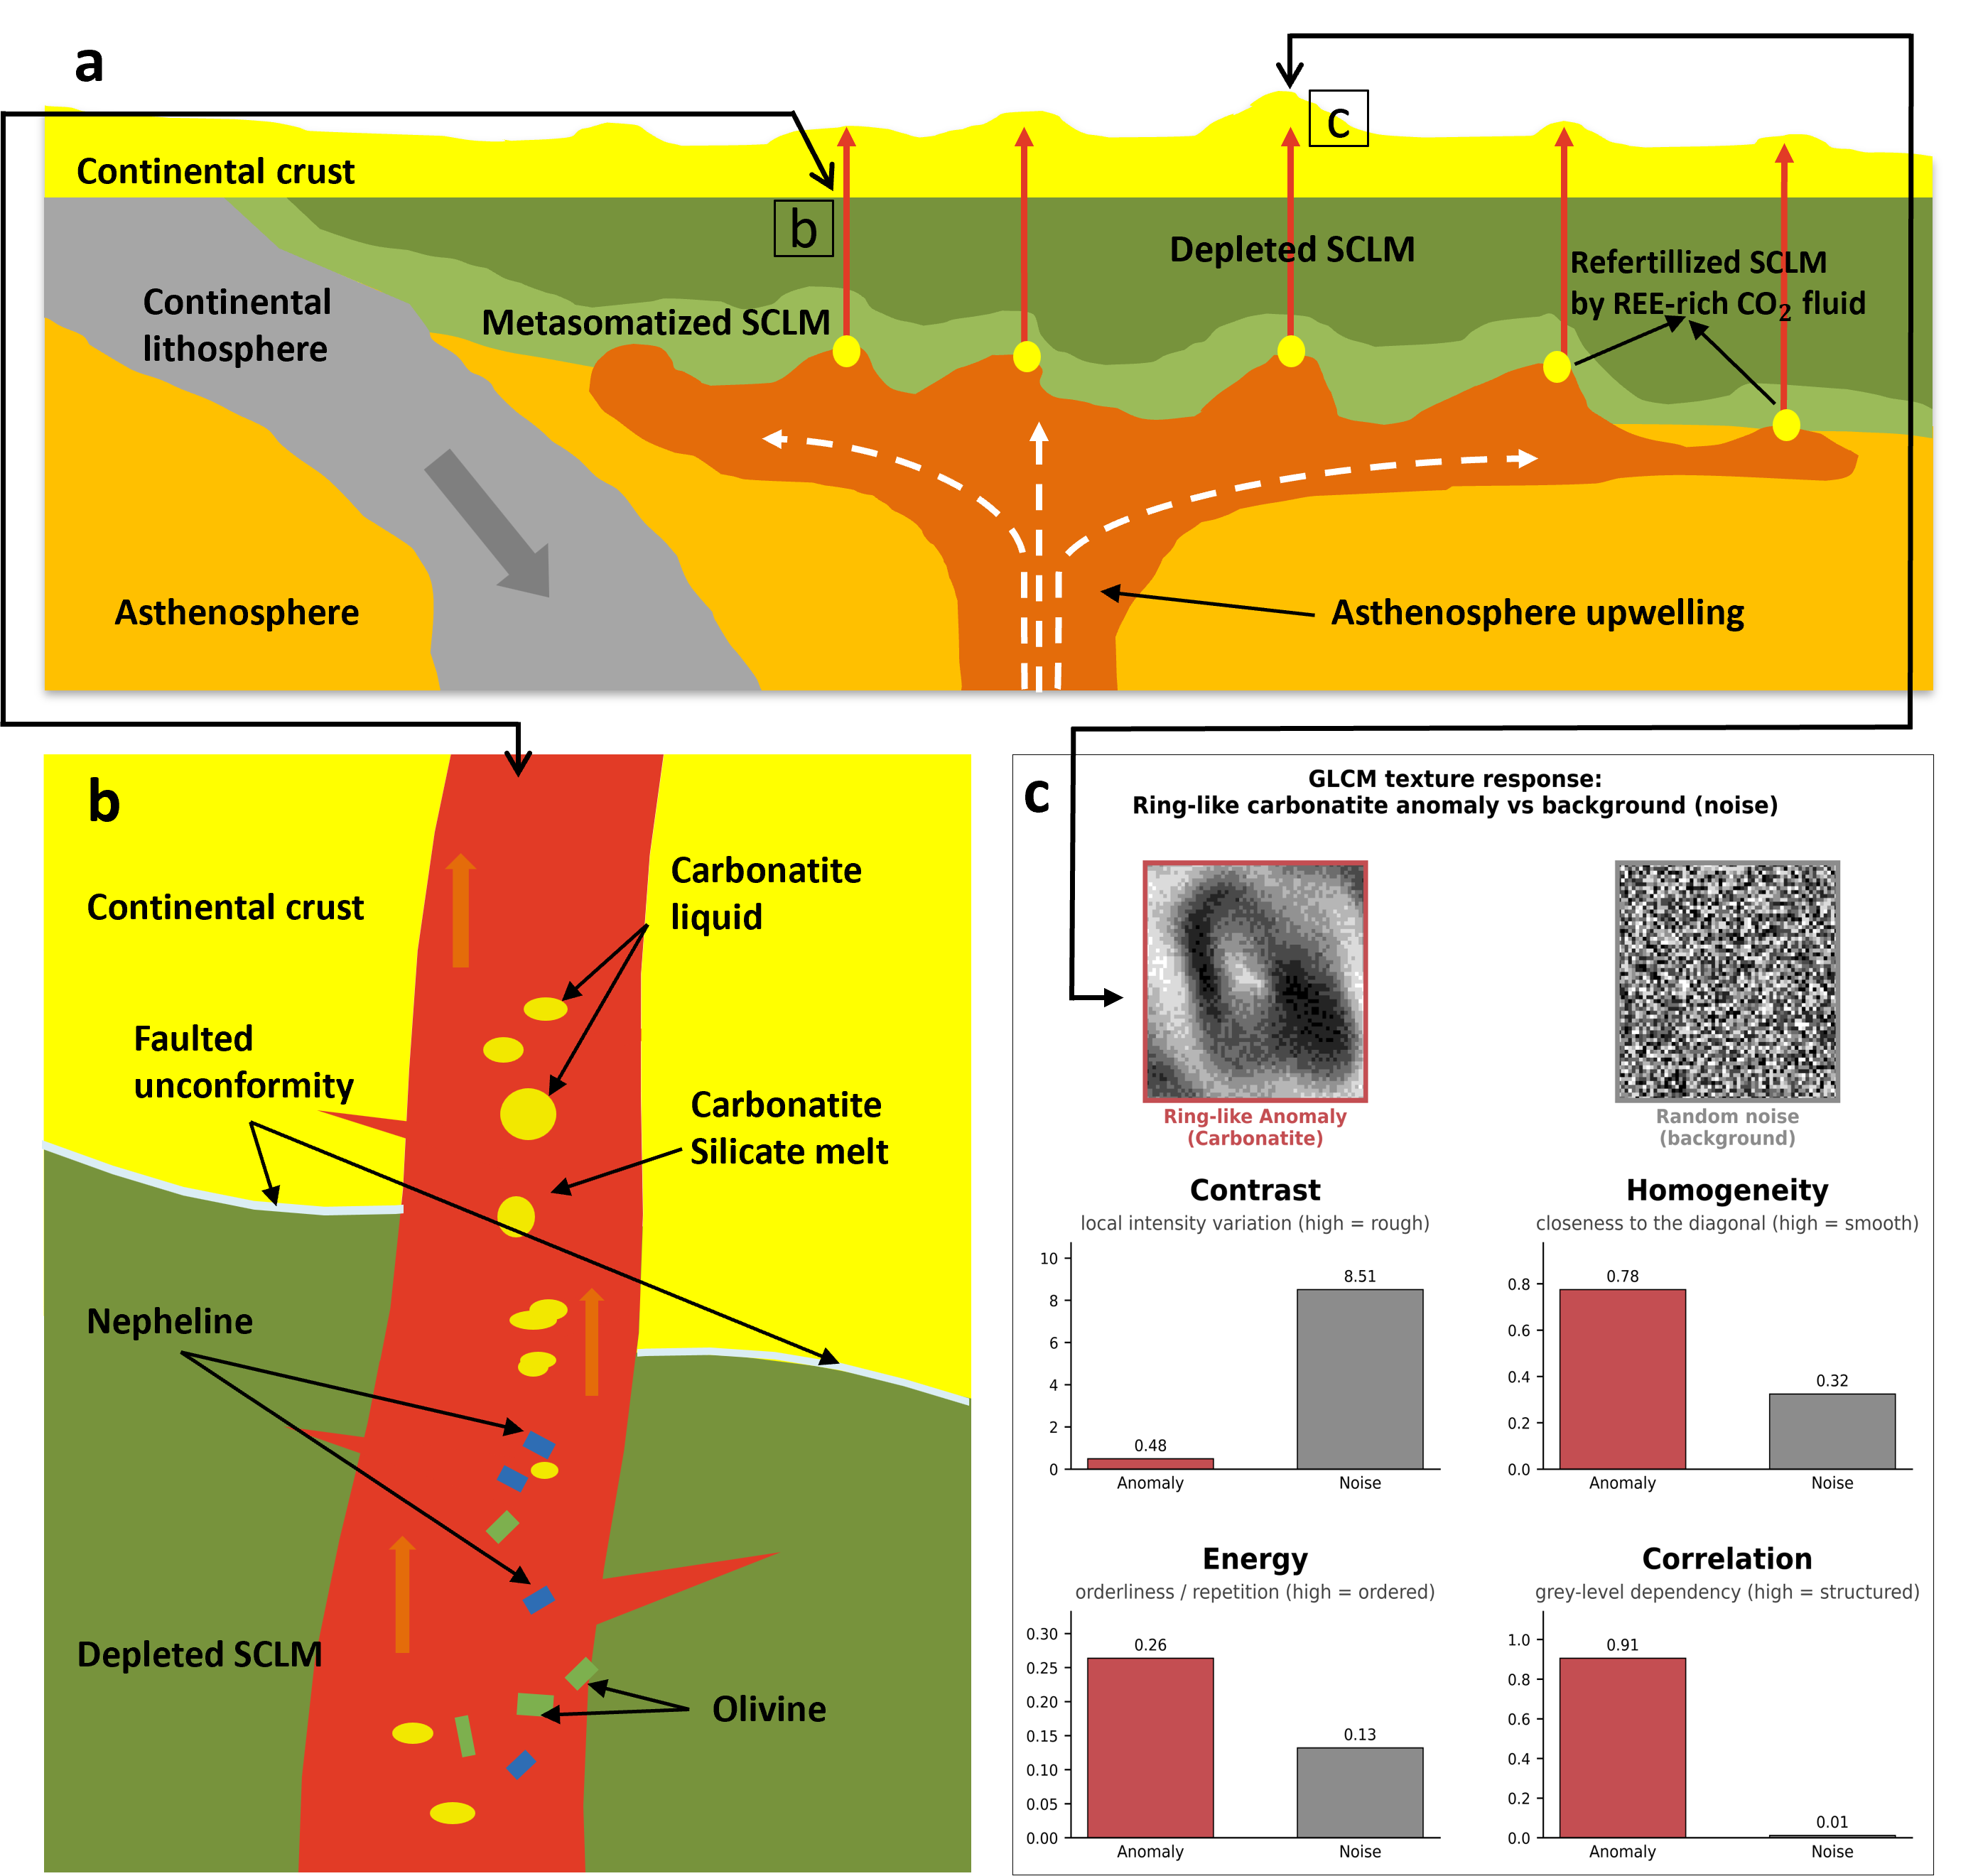
\includegraphics[width=0.85\textwidth]{figures/fig_mineral_system.png}
\caption{碳酸岩型稀土系统的源-运移-圈闭模型及其地球物理代用指标。（a）源：克拉通边缘 LAB 附近经再富集的大陆岩石圈地幔，以 LAB 深度和到克拉通边缘的邻近度表征；该子图据 \citet{Hou2023} 修改。（b）运移：沿穿岩石圈断裂运移，以到断裂和蠕虫的邻近度以及莫霍面深度表征；据 \citet{Yaxley2021} 修改。（c）圈闭：环状异常与随机噪声的 GLCM 纹理响应。}\label{fig:mineral-system}
\end{figure}

\subsection{研究区}\label{sec:areas}

全国研究区为加拿大地质图 \citep[Map 1860A;][]{Wheeler1996} 中陆上地质省、造山带和地台的并集，不含大陆架和洋壳（1230 万 km$^2$）。三个地质省研究区为同一地质图中苏必利尔省、格伦维尔省和科迪勒拉造山带的多边形范围。显生宙增生的科迪勒拉中的碳酸岩型矿点，在地球物理和地质特征上不同于加拿大地盾中的矿点 \citep{Parsa2024}，这意味着单一的跨地体模型可能无法迁移；第~\ref{sec:res-national}~节对此进行了直接检验。被另一地质省包围且面积小于 2,000~km$^2$ 的地质省窗口（如科迪勒拉中 Monashee 和 Malton 杂岩体的丘吉尔基底窗口）被归入其周围的地质省。

苏必利尔省是世界上最大的太古宙克拉通。加拿大地盾中的碳酸岩-碱性岩浆作用集中于约 2.68~Ga、1.90--1.88~Ga 和 1.16--1.08~Ga 几期 \citep{Rukhlov2010}；在苏必利尔省，许多杂岩体沿地壳尺度构造呈线状排列，其中最突出的是卡普斯卡辛构造带 \citep[KSZ;][]{Percival1994,Gittins1967}。本文使用的 15 个苏必利尔省矿点（图~\ref{fig:study}b）包括：魁北克省阿比蒂比地区东部 Montviel 和 Lac Shortt 碳酸岩周围的一个矿点簇（属矿床/远景区类与矿化显示类，即 Deposit/Prospect 和 Showing），以及分散于苏必利尔省南部和西部的矿点，包括 Nemegosenda Lake、Lackner Lake、Kapuskasing、Martison Lake、Prairie Lake 和 Carb Lake。因此，苏必利尔省兼具两个特点：在三个地质省中单位面积矿点数最少；其空间结构为一个紧密的矿点簇加若干分散的孤立矿点，在这种结构下，模型既可能学到该矿点簇，也可能学到分散矿点之间的共性。

\begin{figure}[t]
\centering
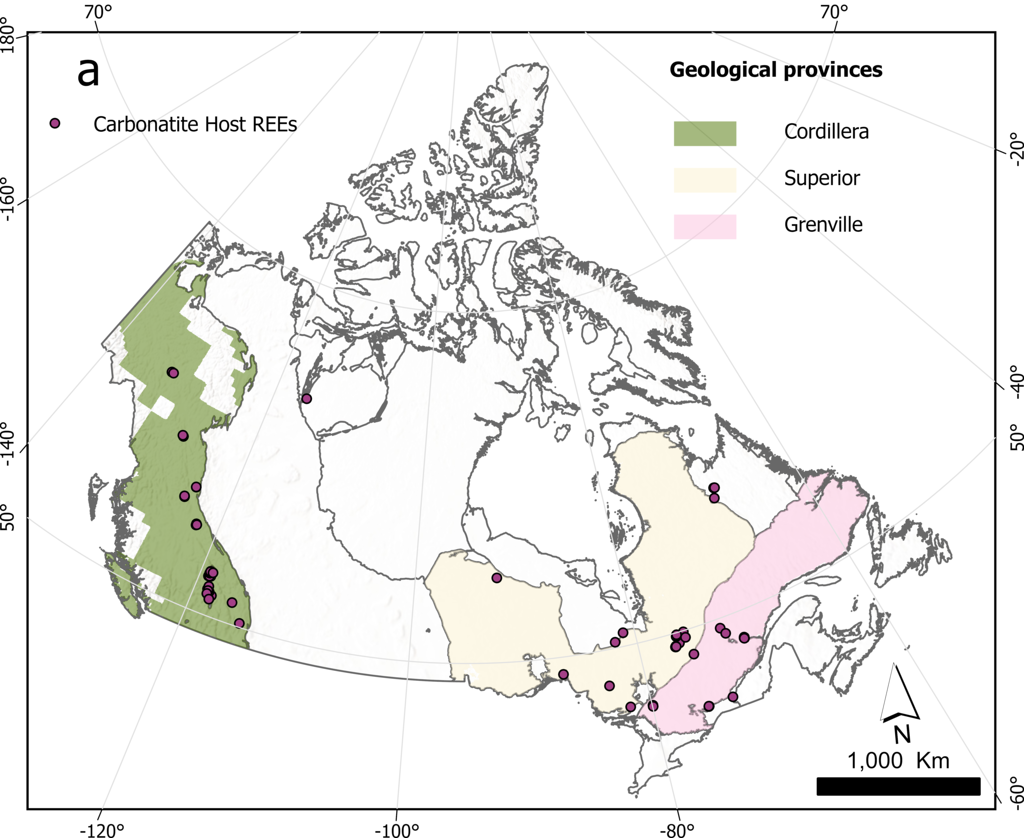
\includegraphics[width=0.55\textwidth]{figures_r7/ree_distribution_1024.png}\hfill
\vspace{0.3cm}
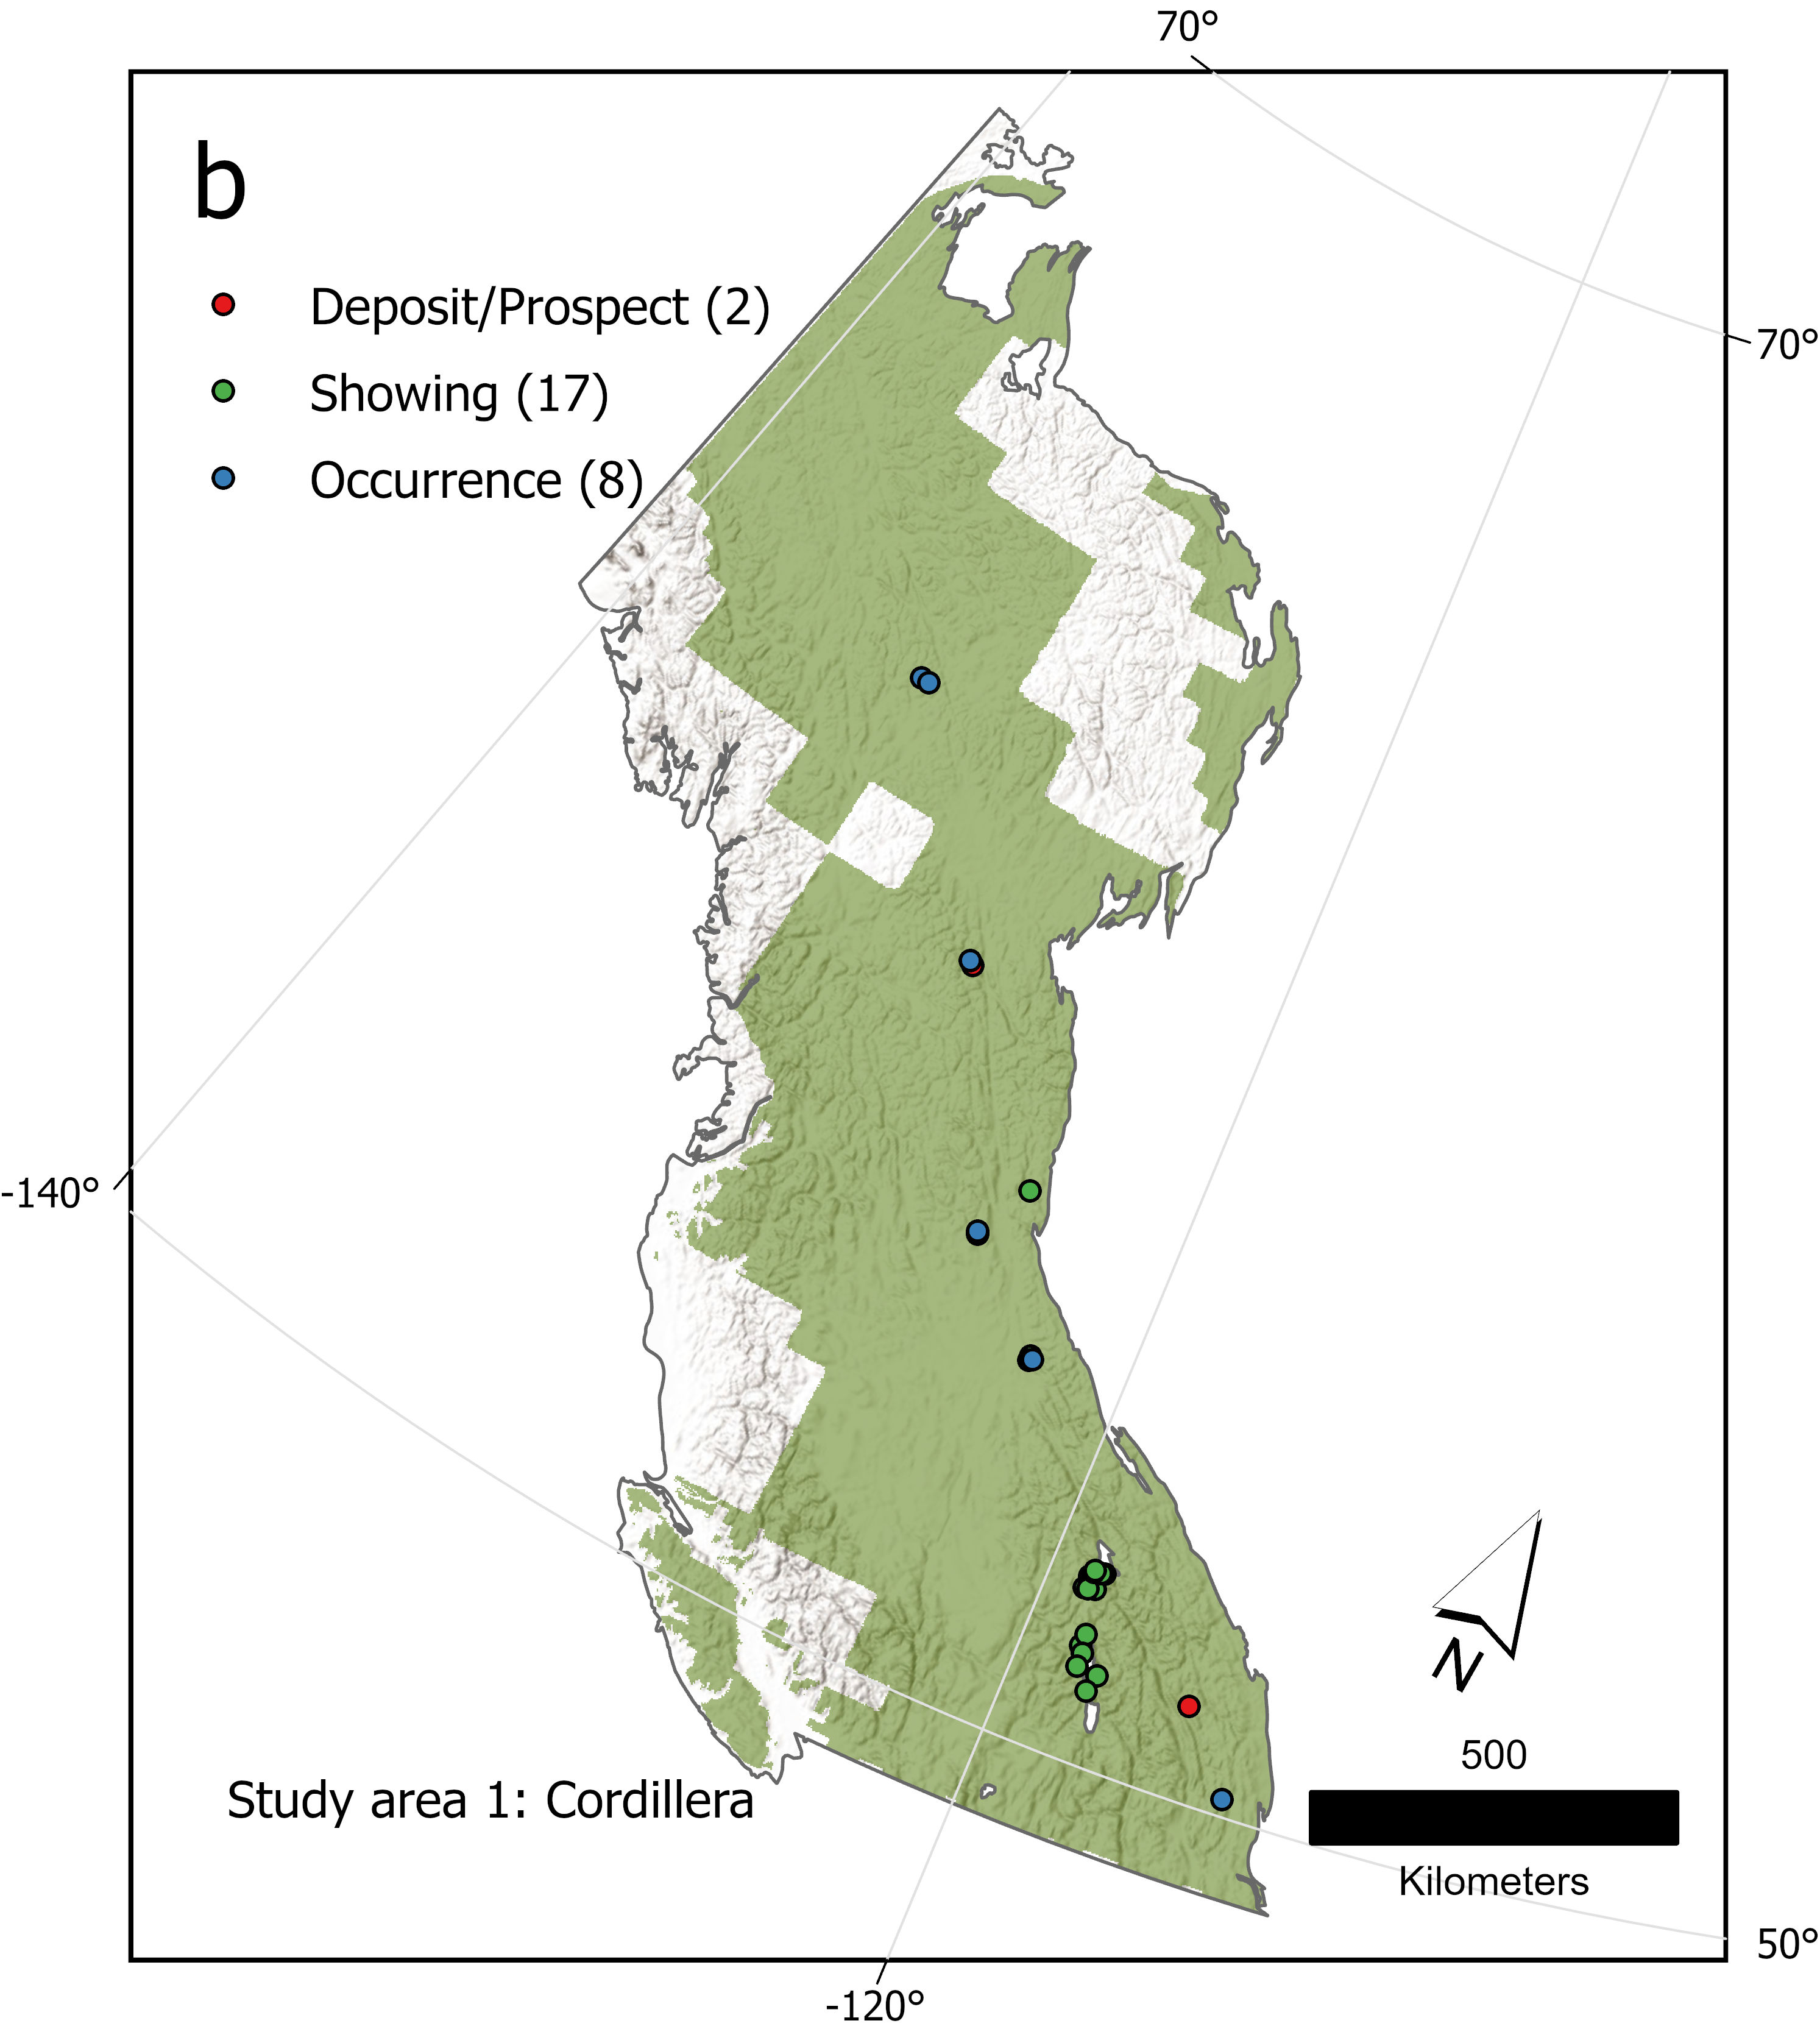
\includegraphics[width=0.42\textwidth]{figures_r7/occurrences-cordillera.jpg}\hfill
\vspace{0.3cm}
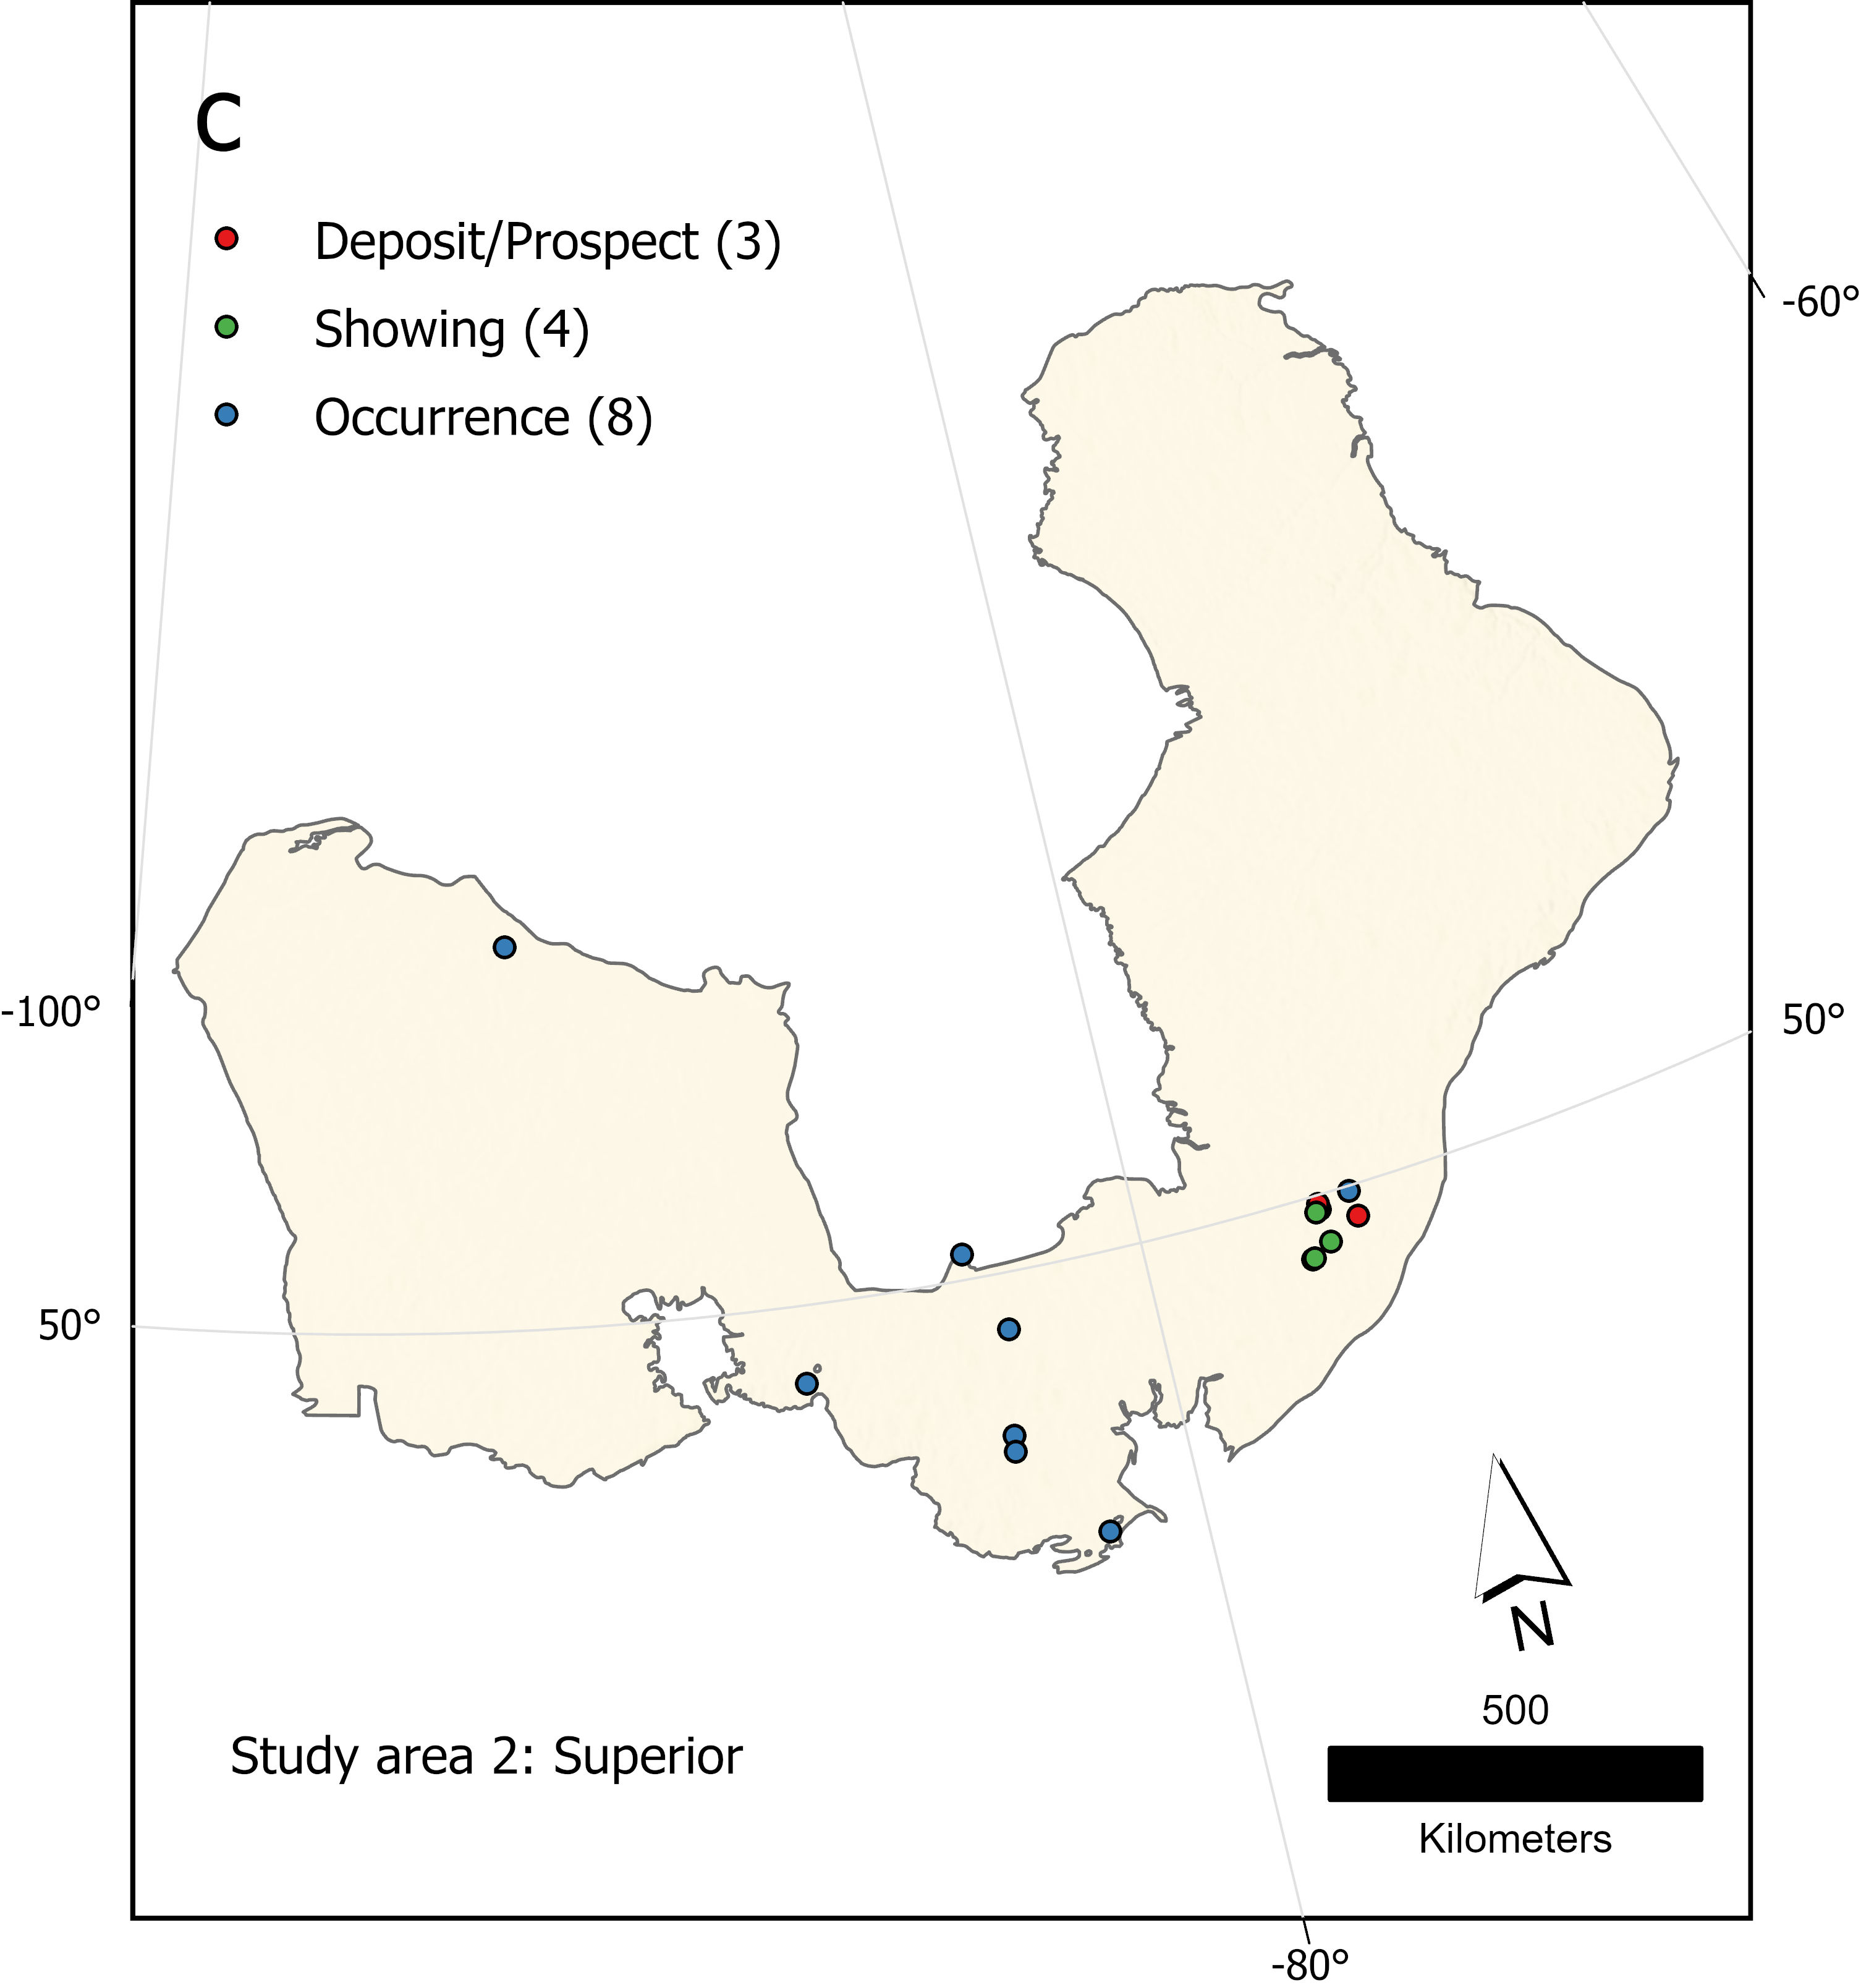
\includegraphics[width=0.427\textwidth]{figures/fig_study_superior.jpg}\hfill
\vspace{0.3cm}
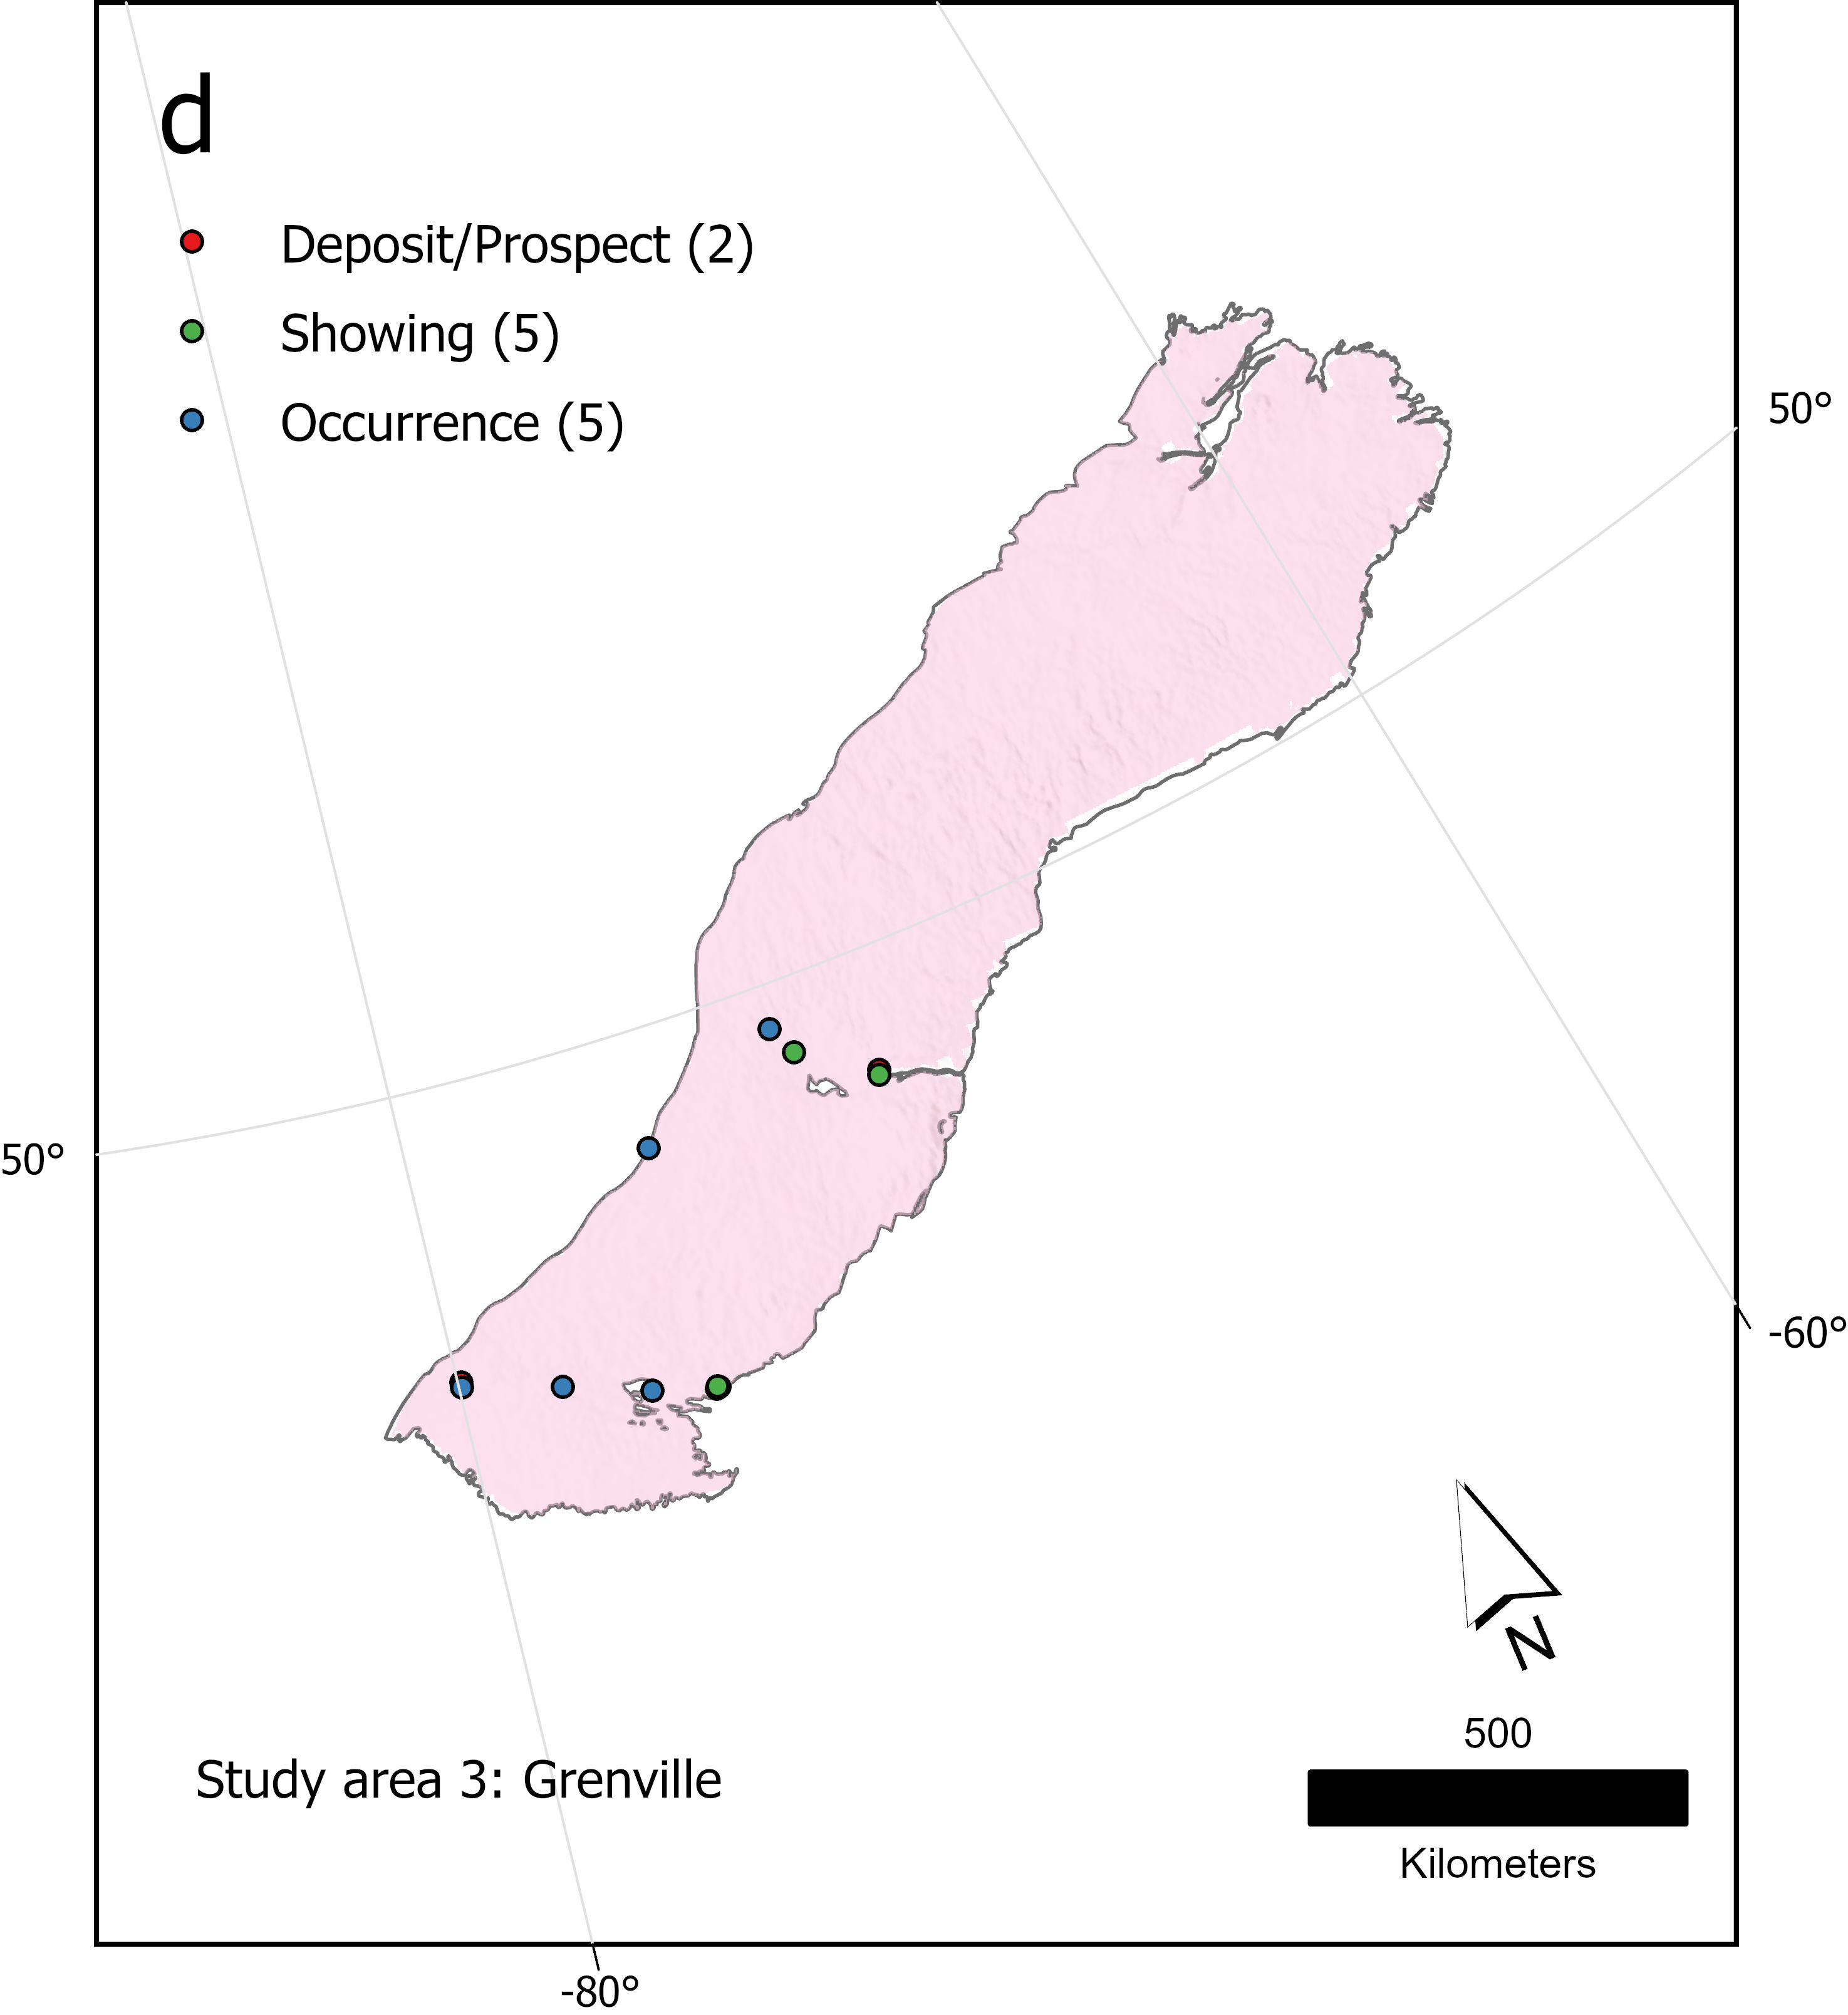
\includegraphics[width=0.42\textwidth]{figures_r7/occurrences-grenville.jpg}
\caption{加拿大全境（a）与三个重点区域（b-d）及已知稀土矿点的对比，显示了加拿大稀土矿化高度不均匀且受地质控制的空间分布。着色区域表示现有数据覆盖的范围（可采样区域），采样和预测均限于该范围内。矿点汇编自两个来源：\citet{Parsa2024} 和 \citet{Orris2018}。符号按 \citet{Parsa2024} 的划分表示各矿点的开发状态：Deposit/Prospect（矿床/远景区：矿化前景良好至边界清晰，具有已确认或潜在的经济资源，需进一步详细勘探以圈定）、Showing（矿化显示：具有经济价值的可能性较高，但需要更多勘探）和 Occurrence（矿点：最基本的矿物显示，通常不具经济可行性）。仅经去重和区域过滤后保留的矿点被用作正样本。}\label{fig:study}
\end{figure}

\subsection{矿点标签}\label{sec:labels}

正样本标签汇编自 USGS 全球稀土矿点数据库 \citep{Orris2018} 中的碳酸岩型记录以及 \citet{Parsa2024} 的矿点表，加拿大全境共计 102 条记录。由于初步的留块（leave-block-out）分类表明碱性岩型矿点在地球物理上可与碳酸岩型矿点区分开，故将其排除。相距 2~km 以内的记录通过单链接聚类合并，使同一矿床的钻孔或矿化带（无论只在一个来源中列出还是在两个来源中均有列出）只计一次；若不进行这一步，来自同一矿床的近乎相同的点会同时落入训练折和验证折。每个矿点保留 \citet{Parsa2024} 的开发状态类别：Deposit/Prospect（矿床/远景区）、Showing（矿化显示）或 Occurrence（矿点）。经合并和数据覆盖过滤（第~\ref{sec:domain}~节）后，全国标签表包含 66 个矿点（图~\ref{fig:study}a）。在三个研究地质省内，同样的步骤将汇集的 21、13 和 51 条记录分别缩减为 15 个（苏必利尔省）、12 个（格伦维尔省）和 27 个（科迪勒拉）正样本；其余 12 个矿点位于加拿大其他地区。

\subsection{地球物理与构造证据图层}\label{sec:layers}

表~\ref{tab:layers} 列出了各证据图层。十七幅全国栅格覆盖了圈闭和深部构架两个组分：布格重力及其导数和滤波版本、总磁场强度及其差分化极和相应导数 \citep{Jobin2017,Miles2016}，以及来自三国关键矿产填图计划（Tri-National Critical Minerals Mapping Initiative）发布数据的长波长重力和磁力、LAB 深度和莫霍面深度 \citep{McCafferty2023}。布格异常（密度 2.67~g\,cm$^{-3}$，经地形校正）、其一阶垂向导数和总水平导数以及总磁场强度均为加拿大自然资源部（Natural Resources Canada）公开发布的汇编数据 \citep{Jobin2017,Miles2016}，分别重新网格化至 2~km（EPSG:3978）和 0.01$^\circ$。其余七幅重力和磁力网格由本研究基于上述数据计算得到。布格异常的 40 和 100~km 高通版本是在波数域中应用六阶 Butterworth 滤波器 $H(k) = [1 + (k_0/k)^6]^{-1}$ 得到的，其中 $k_0$ 为截止波长的倒数。磁场采用差分化极处理 \citep{ArkaniHamed1988,CooperCowan2005}：将总磁场强度划分为 8$^\circ$ 的图块（重叠 4$^\circ$）进行处理，每个图块投影到 1~km 的方位等距网格上；针对覆盖该图块的九种磁倾角与磁偏角组合计算感应磁化的化极结果 \citep{Blakely1995}，并插值到各节点处的地磁场方向，该方向取自国际地磁参考场 \citep[IGRF-13，历元 2020.0；][]{Alken2021}；最后用余弦渐变窗将各图块融合拼接。一阶垂向导数在波数域中计算，总水平导数（THD）以米制单元尺寸通过中心差分计算，网格的倾斜角则为其垂向导数与总水平导数之比的反正切 \citep{Miller1994,Verduzco2004}；THD 倾斜角图层即 THD 网格的倾斜角。两个线图层（古被动大陆边缘，\citealp{BradleyDC2008}；断裂）和四个点图层（浅部和深部的重力与磁力蠕虫；\citealp{McCafferty2023}）以归一化邻近度的形式输入。在全部十一幅重力和磁力网格上，以 9$\times$9 像素窗口计算 GLCM 对比度、同质性、能量和相关性；特征剪枝（第~\ref{sec:pruning}~节）会剔除其中的冗余特征。参照 \citet{Luo2026}，加入每个点 10~km 范围内布格异常、其 40~km 高通版本、化极磁力和总磁场强度的均值与标准差作为邻域统计量。曾考虑使用放射性测量网格（K、eU、eTh），但因其对研究区的覆盖不完整且不均匀而未采用；全岩地球化学数据过于稀疏，无法为每个图件单元提供取值。\citet{Wheeler1996} 的地质省多边形仅用于界定研究区；未使用到地质省边界距离的特征。

\begin{sidewaystable}
\caption{按成矿系统组分和可填图准则列出的证据图层，及其几何类型、原始分辨率和来源。栅格在其原始投影和分辨率下按点采样；线图层和点图层以归一化邻近度的形式输入。}\label{tab:layers}
\footnotesize
\setlength{\tabcolsep}{3pt}
\begin{tabular*}{\textwidth}{@{\extracolsep\fill}>{\raggedright\arraybackslash}p{1.7cm}>{\raggedright\arraybackslash}p{2.6cm}>{\raggedright\arraybackslash}p{3.5cm}>{\raggedright\arraybackslash}p{1.4cm}>{\raggedright\arraybackslash}p{2.4cm}>{\raggedright\arraybackslash}p{7.3cm}>{\raggedright\arraybackslash}p{2.9cm}}
\toprule
组分 & 可填图准则 & 图层 & 几何类型 & 原始分辨率 & 描述 & 来源 \\
\midrule
源 & 克拉通边缘的地幔熔融 & 古被动大陆边缘 & 线 & -- & 到古被动大陆边缘的邻近度 & \citet{BradleyDC2008} \\
 & 岩石圈构架 & LAB 深度 & 栅格 & 0.1$^\circ$（$\approx$11.1~km） & 岩石圈-软流圈边界的深度 & \citet{McCafferty2023} \\
 & 深部地壳构架 & BA 向上延拓 30~km & 栅格 & 0.031$^\circ$（$\approx$3.4~km） & 向上延拓 30~km 的布格重力 & \citet{McCafferty2023} \\
 & & BA 向上延拓 30~km HGM & 栅格 & 0.031$^\circ$（$\approx$3.4~km） & 向上延拓重力的水平梯度模 & \citet{McCafferty2023} \\
 & & 深源 RTP & 栅格 & 0.018$^\circ$（$\approx$2.0~km） & 长波长（深源）化极磁力 & \citet{McCafferty2023} \\
 & & 深源 RTP HGM & 栅格 & 0.019$^\circ$（$\approx$2.1~km） & 深源 RTP 的水平梯度模 & \citet{McCafferty2023} \\
\midrule
%% TODO(author): confirm the provenance of the fault compilation (KNOWN_ISSUES.md #3)
运移 & 地壳构架 & 莫霍面深度 & 栅格 & 0.25$^\circ$（$\approx$27.8~km） & 莫霍面深度 & \citet{McCafferty2023} \\
 & & 断裂 & 线 & -- & 到断裂的邻近度 & \citet{McCafferty2023} \\
 & & 浅部重力蠕虫 & 点 & -- & 到布格重力水平梯度极大值的邻近度 & \citet{McCafferty2023} \\
 & & 深部重力蠕虫 & 点 & -- & 到 30~km 向上延拓重力水平梯度极大值的邻近度 & \citet{McCafferty2023} \\
 & & 浅部磁力蠕虫 & 点 & -- & 到浅部磁源水平梯度极大值的邻近度 & \citet{McCafferty2023} \\
 & & 深部磁力蠕虫 & 点 & -- & 到深部磁源水平梯度极大值的邻近度 & \citet{McCafferty2023} \\
\midrule
圈闭 & 重力异常 & 布格异常（BA） & 栅格 & 2~km & 布格异常（2.67~g\,cm$^{-3}$，经地形校正） & \citet{Jobin2017} \\
 & & BA 1VD & 栅格 & 2~km & BA 的一阶垂向导数 & \citet{Jobin2017} \\
 & & BA THD & 栅格 & 2~km & BA 的总水平导数 & \citet{Jobin2017} \\
 & & BA THD 倾斜角 & 栅格 & 2~km & BA THD 的倾斜角 & 本研究 \\
 & & BA 高通 40~km & 栅格 & 2~km & BA 的 40~km 高通滤波（六阶 Butterworth） & 本研究 \\
 & & BA 高通 100~km & 栅格 & 2~km & BA 的 100~km 高通滤波（六阶 Butterworth） & 本研究 \\
\cmidrule(l){2-7}
 & 磁异常 & 总磁场强度（TMI） & 栅格 & 0.01$^\circ$（$\approx$1.1~km） & 总磁场强度 & \citet{Miles2016} \\
 & & DRTP & 栅格 & 0.01$^\circ$（$\approx$1.1~km） & TMI 的差分化极 & 本研究 \\
 & & DRTP 1VD & 栅格 & 0.01$^\circ$（$\approx$1.1~km） & DRTP 的一阶垂向导数 & 本研究 \\
 & & DRTP THD & 栅格 & 0.01$^\circ$（$\approx$1.1~km） & DRTP 的总水平导数 & 本研究 \\
 & & DRTP THD 倾斜角 & 栅格 & 0.01$^\circ$（$\approx$1.1~km） & DRTP THD 的倾斜角 & 本研究 \\
\cmidrule(l){2-7}
 & 异常几何形态 & GLCM 纹理 & 派生 & 9$\times$9 像素窗口 & 十一幅重力和磁力网格各自的对比度、同质性、能量和相关性 & 本研究 \\
 & & 邻域统计量 & 派生 & 10~km 半径 & BA、BA 高通 40~km、DRTP 和 TMI 的均值与标准差 & 本研究，参照 \citet{Luo2026} \\
\cmidrule(l){2-7}
 & 赋矿构架 & 岩性、时代、接触带 & H3 网格 & 分辨率 7（$\approx$4.9~km$^2$ 单元） & 单元的主要岩性类别和时代（独热编码）；单元内岩性接触带和年代接触带的标志 & \citet{Wheeler1996} \\
 & & 到概化地质的距离 & 派生 & -- & 到岩性接触带和年代接触带，以及到绿岩、镁铁质-超镁铁质、高级变质和沉积单元的距离（第~\ref{sec:featuresets}~节） & 本研究，基于 \citet{Wheeler1996} \\
\botrule
\end{tabular*}
\end{sidewaystable}

\subsection{地质}\label{sec:featuresets}

地质信息来自一个依据加拿大地质图 \citep{Wheeler1996} 赋予属性的六边形 H3 网格（分辨率 7，单元面积约 5~km$^2$）。每个单元带有一个主要岩性类别（例如 Igneous Intrusive Alkalic，即碱性侵入岩；或 Metamorphic Gneiss Paragneiss，即变质片麻岩-副片麻岩）、其主导时代，以及标示该单元是否被岩性接触带或年代（纪）接触带穿过的标志；每个点取其所在单元的属性。岩性类别以独热编码列的形式输入（若区域内 5,000 个训练背景点中至少有 10 个落入某一类别，则该类别单独占一列；更少见的类别共用一列），同时输入时代的独热编码和两个接触带标志。参照 \citet{Luo2026}，地质信息还以到概化地质图中六类要素的距离（km）的形式输入；该概化图剔除了所有小于 20 个相连单元（约 100~km$^2$）的岩性单元以及碱性侵入体类别。这六类要素为：岩性接触带、年代接触带、绿岩（喷出岩）单元、镁铁质-超镁铁质侵入体、高级变质单元和沉积单元。经剪枝（第~\ref{sec:pruning}~节）后，苏必利尔省的输入为 57 个（33 个地球物理和构造图层，其中 14 个为 GLCM 纹理；3 个邻域统计量；2 个区域距离；15 个岩性列；2 个时代列；2 个接触带标志），科迪勒拉为 61 个，格伦维尔省为 66 个。

在碳酸岩杂岩体的尺度上，基岩地质图可能直接标示出目标本身：在苏必利尔省，15 个矿点中有 6 个落在被填绘为碱性侵入岩的单元上，而 3,000 个评估背景点中仅有 16 个（0.5\%）。对勘探者而言，已填图的碱性杂岩体是合理的证据，但模型仅靠“查找”它即可获得高分。因此，我们还报告了不使用点位级地质图类别（岩性、时代和接触带列）的模型结果，仅保留地球物理和构造图层、邻域统计量和区域距离（剪枝后分别为 38、37 和 41 个输入）。这衡量的是模型在地质图未显示杂岩体的区域所能达到的表现。

\subsection{可采样区域与背景}\label{sec:domain}

栅格按各研究区轮廓向外缓冲一个 GLCM 窗口半径（8~km）后进行裁剪，使边界附近的窗口读取的是真实数据；采样和预测被限制在所有图层均有数据且所有纹理窗口均可计算的区域内。该区域覆盖苏必利尔省轮廓的 98.6\%、格伦维尔省轮廓的 97.2\%、科迪勒拉轮廓的 73.5\%，以及加拿大的 809 万 km$^2$（65.6\%）；一个科迪勒拉矿点（Lempriere）和一个圣劳伦斯地台矿点（Francon Quarry）落在该区域之外，因而被剔除。背景候选点为该区域内 0.1$^\circ$ 网格上距任一已知矿点超过 10~km 的节点（苏必利尔省为 19,371 个）。从中为每个区域一次性随机抽取两个互不相交的样本池：3,000 个点的评估背景和 5,000 个点的训练背景。本研究中的每个模型都以其训练折中的正样本加上同一组 5,000 个训练背景点进行训练，并在留出的正样本加上同一组评估背景上进行评分。因此，在苏必利尔省，评分样本池中的正样本比例为 15/3,015 $\approx$ 0.5\%，这也就是随机排序的 AP。

全国尺度分析对整个加拿大采用相同的规则。在各研究地质省内，全国背景点即该省的背景点（在科迪勒拉和格伦维尔省中取其随机子集，使密度与苏必利尔省一致）；在其他地区，按苏必利尔省的密度（即候选节点的 41\%）抽取背景点，并与各地质省一样，将评估背景与训练背景按 3:5 划分。全国数据表包含 66 个矿点、20,855 个评估背景点和 34,761 个训练背景点（正样本比例 0.32\%）。

%% ===================================================================
\section{方法}\label{sec:methods}

图~\ref{fig:workflow} 概括了工作流程。所有分析的代码，包括每个表格中确切数值的生成代码，均可在“代码可用性”部分列出的代码仓库中获取。

\begin{figure}[t]
\centering
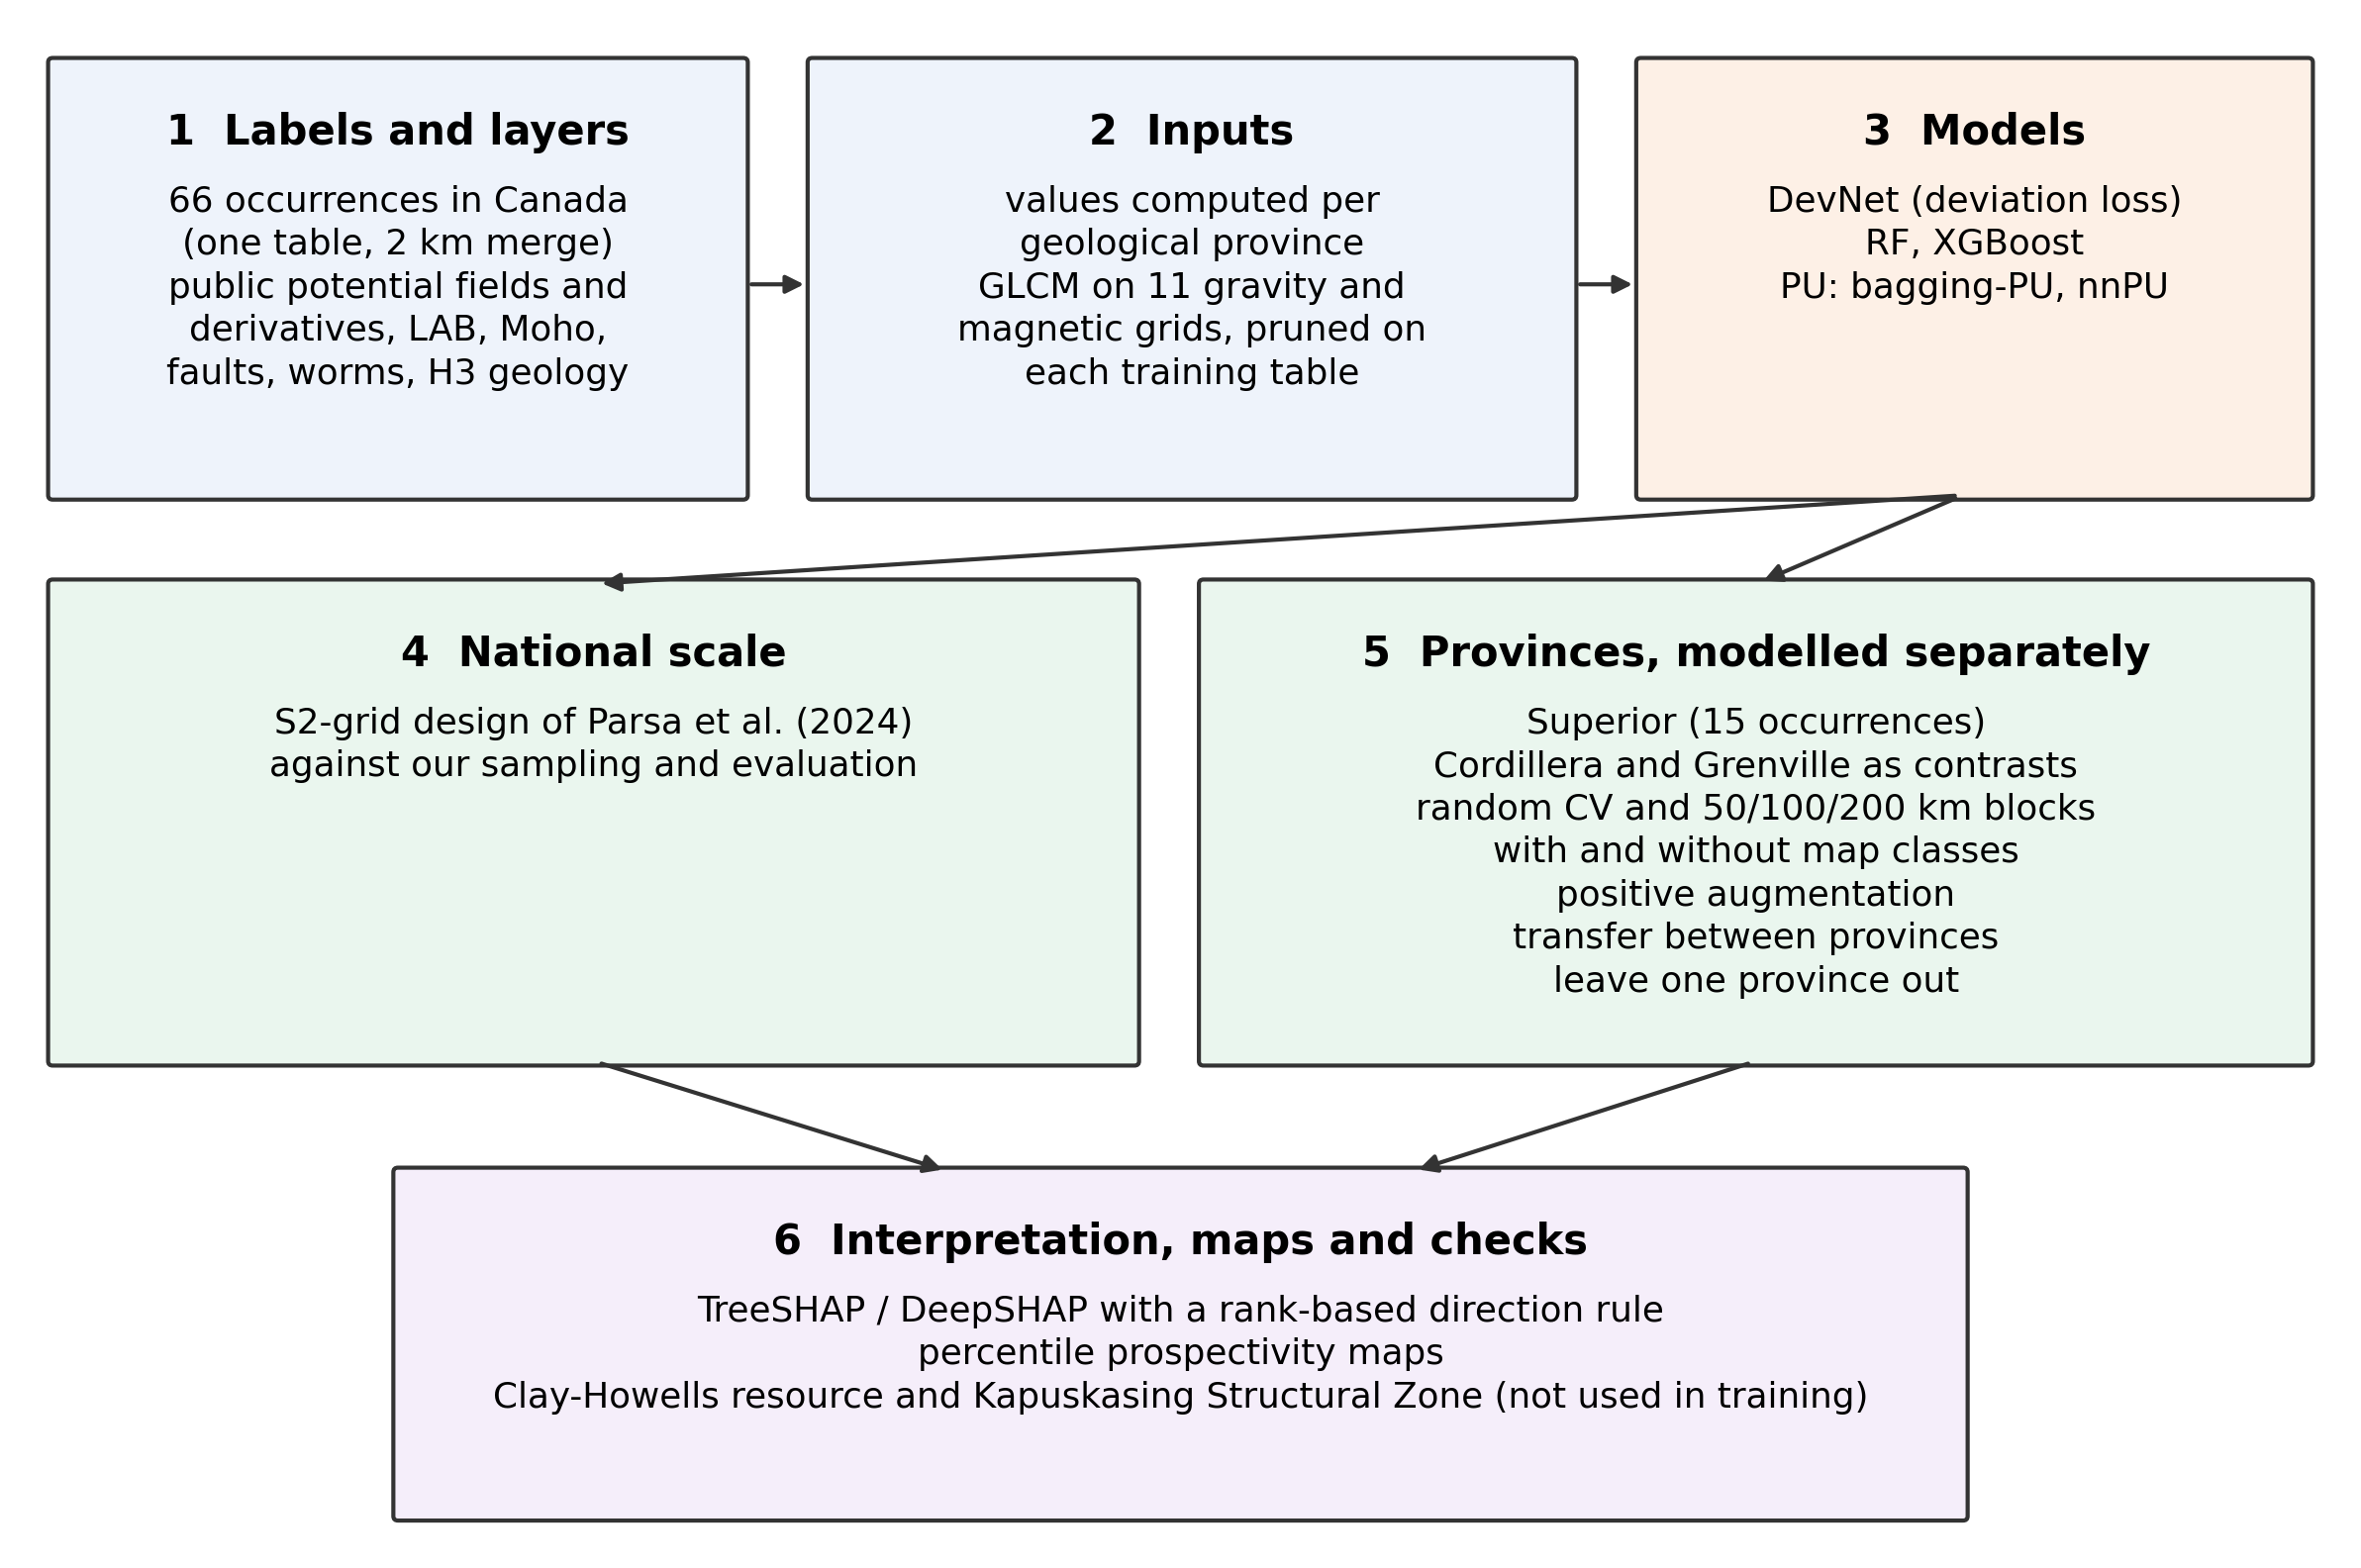
\includegraphics[width=\textwidth]{figures_r7/fig_workflow_r7.png}
\caption{工作流程。全国尺度实验比较不同的采样设计；各省分别建模，并用省级模型检验省际迁移。在同一组比较中，所有模型均使用相同的正样本和背景训练，并在相同的折上评分；唯一的区别在于对背景的处理方式。}\label{fig:workflow}
\end{figure}

\subsection{全国与省级输入}\label{sec:framework}

有三类输入取决于其计算所覆盖区域的范围：裁剪边缘处的栅格值（中心落在缓冲后轮廓之外的粗分辨率像元为无数据值）；GLCM 灰度级，其在裁剪后栅格的第 2 至第 98 百分位数之间量化；以及概化地质图，其由轮廓外包矩形加外扩边距范围内的 H3 单元构建。这三者均按地质省分别计算，研究省采用省级栅格和外包矩形，从而使每个全国尺度的值都与同一点的省级值相等。特征剪枝（第~\ref{sec:pruning}~节）和 H3 类别列表作用于模型训练所用的数据表：全国模型使用在全国数据表上剪枝后的 71 个输入，而某省的模型使用该省的输入和网络容量，即使将其应用于另一省时也是如此。

\subsection{特征剪枝}\label{sec:pruning}

候选特征中包含许多相互共线的地球物理导数图层。在每个区域内，以 $1-|\rho_{\mathrm{S}}|$ 为距离（Spearman 相关系数，平均连接法）对特征进行层次聚类，并在 $|\rho_{\mathrm{S}}| = 0.7$ 处切割，每个簇保留一个代表特征，优先选择缺失率最低者，其次选择方差最大者 \citep{Dormann2013}。该规则从不使用标签，因此不会在折之间泄漏信息。

\subsection{模型}\label{sec:models}

所有模型使用相同的数据行，区别仅在于对训练背景的处理方式或损失函数。

\textbf{随机森林}（RF；\citealp{Breiman2001}）是判别式基线模型：将正样本与标记为 0 的训练背景进行区分，使用 300 棵树，每次分裂考虑 $\sqrt{p}$ 个特征，采用平衡类别权重，并置于一个仅在训练折上拟合中位数插补和标准化的流水线中。由于约 12 个训练正样本对应 5,000 个背景点，大多数留出点的预测概率恰好为零，因此汇总的 AUC 取决于哪些树恰好为某个留出矿点投票。为此，我们在不同折之间改变 RF 的随机种子，使这一方差反映在所报告的区间中。

\textbf{XGBoost} \citep{Chen2016} 增加了一个梯度提升树集成模型，其参数沿用同一矿种的一项并行全国尺度研究中预先确定的设置，而未在本文中调参：200 棵深度为 2 的树，学习率 0.1，行和列子采样比例 0.8，最小子节点权重 3，L2 和 L1 惩罚分别为 2 和 0.5。其训练方式与 RF 相同：使用中位数插补后的输入，并提高正样本权重以平衡两个类别。

\textbf{DevNet} \citep{Pang2019} 通过一个带 dropout 的 ReLU 隐藏层，将每个输入向量 $\mathbf{x}$ 映射为标量得分 $\phi(\mathbf{x})$。偏差 $d(\mathbf{x}) = (\phi(\mathbf{x}) - \mu_R)/\sigma_R$ 相对于一个固定参考样本（50,000 个标准正态抽样值）的均值和标准差来度量，损失函数
\begin{equation}
L = (1-y)\,|d(\mathbf{x})| + y\,\max\{0,\, a - d(\mathbf{x})\}
\end{equation}
将无标签背景（$y=0$）拉向参考分布，并将正样本（$y=1$）推至间隔（margin）$a = 5$ 之外，该取值即 \citet{Pang2019} 所用的值（附录~\ref{app:sensitivity}，表~\ref{tab:margin}）。网络容量根据正样本数量预先设定（科迪勒拉为 64 个隐藏单元、dropout 0.3、权重衰减 $10^{-4}$；苏必利尔省和格伦维尔省为 32、0.4 和 $10^{-3}$），而非通过调参得到，因为在仅几十个正样本上进行搜索只会拟合噪声。训练采用带权重衰减的 Adam 优化器 \citep{Kingma2014}，在 300 步内进行余弦学习率退火，并使用梯度裁剪；每一折的得分为五次使用不同随机种子的重启结果的秩平均。

有两项设计选择使 DevNet 适用于正样本极少的表格型证据图层。第一，通过在每个训练折上拟合的分位数变换，将输入映射为标准正态边缘分布。许多证据图层呈强烈偏态（集中于 0 或 1 附近的反转距离、长尾的纹理特征、0/1 哑变量）；树集成模型对单调变换具有不变性，而多层感知机则与之不同，对此类边缘分布较为敏感 \citep{Gorishniy2021,Grinsztajn2022}。第二，每个梯度步使用 16 个正样本（有放回重采样）和 240 个背景行。偏差损失旨在学习背景的样貌；若使用 16 + 16 行的标签平衡批次，300 步训练中每个背景行仅出现约一次，而每个正样本出现约 400 次；以背景为主的批次则使每个背景行出现约 14 次，而正样本的出现次数保持不变。这两项选择均是根据在这些省份上采用较早、较粗略的地质编码所进行的诊断性运行确定的；附录~\ref{app:sensitivity} 使用本文所用的输入重复了该消融实验。

\textbf{Bagging-PU} \citep{Mordelet2014} 训练 200 棵完全生长的决策树，每棵树使用全部训练正样本以及从无标签背景中抽取的等量自助样本，并对各树输出取平均。它是标准的基于树的 PU 学习方法，也是与 RF 最接近的 PU 对应方法。

\textbf{nnPU} \citep{Kiryo2017} 以 sigmoid 损失最小化非负 PU 风险，并采用与 DevNet 完全相同的网络、分位数-正态变换后的输入、优化器、步数和五次重启集成，从而使 DevNet 与 nnPU 的比较能够将 PU 风险与偏差损失的作用区分开来。nnPU 需要无标签总体中的类别先验 $\pi = P(y=1)$；我们取 $\pi = 0.01$（敏感性分析见附录~\ref{app:full}，表~\ref{tab:prior}）。本文未纳入 \citet{Elkan2008} 的校准方法，因为在其假设下，校准后的输出是正样本-背景分类器输出的单调变换，因此其排序以及本文报告的所有基于排序的指标都与 RF 相同。

\subsection{评估方案}\label{sec:protocol}

由于每个验证折中仅有三到四个正样本，逐折计算的 AUC 不稳定，甚至可能无法定义，因此我们汇总折外得分 \citep{BradleyAP1997}：每个留出点在每次重复中被评分一次，得分被转换为折内百分位秩以使各折可比，然后在所有折上计算单一的 AUC 和平均精度（AP）。已知汇总会使 AUC 产生轻微的负偏差 \citep{Airola2019,Parker2007}。我们侧重 AP，因为在 0.5\% 的正样本比例下，它反映了将矿点集中于较小搜索区域这一实际任务，而 AUC 则主要受大量易于排除的背景主导 \citep{Saito2015}。勘查效率还以捕获率曲线表示，即留出矿点中排名位于评分样本池给定前若干比例之内者所占的比例 \citep{Chung2003,Agterberg2005}。由于评估背景是研究区域的随机样本，该比例近似于搜索面积。由于未勘查的背景中可能赋存尚未发现的矿点，所有指标都是保守的。

\textbf{随机交叉验证。}采用六次重复的分层 5 折交叉验证，每个模型得到六个汇总的 AUC 和 AP 值，以各次重复的中位数及 2.5--97.5 百分位区间（标记为 95\% 区间）报告。所有模型使用完全相同的划分，因此可以进行两两比较。

\textbf{空间分块交叉验证。}随机划分的折可能将距某一训练矿点仅数千米的矿点留出。参照 \citet{Roberts2017} 和 \citet{Valavi2019}，在 Canada Atlas Lambert 投影（EPSG:3978）中将有标签的点分配到边长为 50、100 或 200~km 的正方形分块中，采用分层分组 5 折划分将整个分块一同留出（若含正样本的分块较少，则减少折数），并在该折中将落入留出分块内的所有训练背景点从训练集中移除。六次重复中的每一次都对分块网格施加一个随机偏移。

\textbf{配对比较。}对于每一对模型，我们将每个点的折外秩在六次重复上取平均，并对正样本和背景进行 5,000 次分层自助重采样 \citep{Efron1993}，报告 AP 和 AUC 的差值及其 95\% 百分位区间，以及在六次重复中第一个模型 AP 较高的次数。由于仅有 12--27 个正样本，这些比较的统计功效很低，因此只有当差异在各次重复、各分块尺寸和各省之间均保持一致时，我们才认为该差异成立。

\subsection{全国尺度实验}\label{sec:national-methods}

\textbf{采样与增强。}我们使用相同的几何库，在中心位于全国研究区域内的每个第 12 级 S2 单元（约 4.5~km$^2$）上（共 1,616,693 个单元）重建了 \citet{Parsa2024} 的全国 S2 网格设计，输入在单元中心提取；66 个矿点落在 66 个单元中。与原研究一致，每个矿点单元被替换为其四个第 13 级子单元；从在 min--max 缩放特征空间中与正样本平均余弦相似度最低的 5\% 单元中抽取等量的负样本；并在 min--max 缩放后的输入上，以增强标签 50 次分层 70/30 划分的测试 AUC 评估原研究的两种分类器，即包含 1,000 棵树的随机森林（该设置位于原研究网格搜索的范围内，我们未重复该网格搜索），以及该研究的最佳模型——一维 CNN，包含一个卷积层（512 个宽度为 5 的滤波器，带批归一化和 dropout）、最大池化、256、128 和 64 个单元的全连接层以及 sigmoid 输出，采用 Adam 优化器以均方误差损失训练并使用早停。原研究未报告的 CNN 设置由我们自行确定：池化大小 2、dropout 0.3、批次大小 32、学习率 $10^{-3}$，并在分层抽取的 20\% 训练标签上连续 20 个轮次（epoch）无改进时早停。在我们的设计中，同样的两个模型采用类别平衡设置（随机森林使用平衡类别权重，CNN 在每个轮次中进行类别平衡重采样），以每个矿点单元一个标签、对比 34,761 个距任一矿点超过 10~km 的随机抽样单元进行训练，并在留出的 30\% 矿点单元以及从另一个不相交的 20,855 个单元样本中随机抽取的 30\% 上进行测试，对应约 0.3\% 的真实正样本比例。为确定原设计中哪一要素驱动了其得分，我们还每次只改变一个要素：以随机负样本代替余弦相似度最低的负样本；采用使同一单元的四个子单元位于划分同一侧的划分方式；以及不进行增强。为绘制地图，每种设计与分类器的组合均用其全部标签拟合一次，并对每个 L12 单元评分；同时以 50,000 个随机单元中、在缩放后的输入空间里最近的训练样本为正样本的比例，来刻画每种设计教给模型的是什么。

\subsection{正样本增强}\label{sec:augmentation}

为检验正样本增强能否弥补标签稀缺，在重新训练 RF 和 DevNet 之前，为每个训练折的真实正样本补充 $m \times n_{\mathrm{pos}}$ 个增强正样本（$m = 1, 3, 10$）；留出的正样本始终为真实样本。我们比较了三种生成器，均仅在训练折的标准化特征空间中拟合：对真实正样本施加高斯抖动（$\sigma = 0.1$ 个标准差）；在一个正样本与其三个最近正样本邻居之一之间进行 SMOTE 式插值 \citep{Chawla2002}；以及带梯度惩罚的表格型 Wasserstein GAN \citep[WGAN-GP;][]{Goodfellow2014,Arjovsky2017,Gulrajani2017}，其潜在输入为八维，生成器和判别器（critic）各含两个 64 单元的隐藏层，每次生成器更新对应五次判别器更新，梯度惩罚权重为 10，共进行 2,000 次生成器更新，在该折的 12 个正样本上训练。增强正样本的地质列被强制还原为有效的独热编码和 0/1 取值。为考察生成器的产出，我们还将每种生成器拟合到苏必利尔省全部 15 个正样本上，并以如下指标刻画所生成的 150 个样本：到最近真实正样本的距离除以真实正样本之间最近邻距离的中位数（接近 0 的值表示复制）；最近有标签邻居为正样本而非背景点的样本所占比例；以及样本的 DevNet 得分百分位。

\subsection{省际迁移}\label{sec:transfer-methods}

用省 A 的模型（其输入、容量、矿点和训练背景）对省 B 的矿点和评估背景进行评分，使用六个随机种子；对角线元素即 A 内部的随机交叉验证，为省级结果。在留一省验证中，用在剔除某一省组（苏必利尔省、科迪勒拉、格伦维尔省或加拿大其余地区）后的全国数据表上训练的模型对该省组进行评分。为描述各省之间的差异，我们用随机森林（300 棵树，5 折交叉验证）尝试区分两个省组的训练背景，以及两个省的矿点；此外，单个输入在区分某省矿点与该省评估背景时的 AUC 给出了该输入在该省指示矿点的方向。

\subsection{解释与制图}\label{sec:shap}

最终（生产）模型使用每个区域的全部正样本和训练背景进行拟合。SHAP 值 \citep{Lundberg2017} 在由全部正样本和评估背景点组成的解释集（共 200 个）上计算，RF 使用 TreeSHAP \citep{Lundberg2020}，DevNet 使用 DeepSHAP，并以 100 个训练背景点作为 DevNet 的参考样本；DevNet 的 SHAP 值针对的是经分位数变换后的输入，这并不影响下文定义的基于秩的方向。DevNet 的 SHAP 值在五个集成成员上取平均。重要性定义为平均 $|$SHAP$|$。特征作用的\emph{方向}定义为解释集上该特征取值与其 SHAP 值之间的 Spearman 相关系数（对于独热编码哑变量，则为存在与不存在时平均 SHAP 值之差的符号），$|\rho| < 0.1$ 时报告为无明确方向。我们不采用平均 SHAP 值的符号，因为它反映的是被解释点相对于解释器基线的位置，而非较高的特征值是否会提高得分：对于使用平衡类别权重的 RF，TreeSHAP 基线接近 0.5，而几乎所有被解释点的得分都接近 0，因此按该规则，RF 的每个特征都会被标记为“越高 $\rightarrow$ 越无远景”。远景图将每个模型在 0.1$^\circ$ 预测网格上的得分划分为前 1\%、前 5\% 和前 10\% 等级，因为 DevNet 的异常得分与 RF 的概率不在同一尺度上。作为外部检验，最终模型在 Clay-Howells 的记录位置对其进行了评分；Clay-Howells 是位于 KSZ 上、经钻探验证并有已报告资源量的 Fe--REE--Nb 远景区 \citep{OGS2011}，不在训练标签之中。

%% ===================================================================
\section{结果}\label{sec:results}

\subsection{全国尺度}\label{sec:res-national}\label{sec:res-ladder}

在我们的全国数据上重建后，\citet{Parsa2024} 的设计无论使用其随机森林还是其 CNN，测试 AUC 均为 1.000（表~\ref{tab:nat-design}），与已发表的 0.91--0.96 一样高甚至更高。若每个矿点单元只取一个标签、采用随机背景并采用真实正样本比例，随机森林的 AUC 为 0.903、AP 为 0.292，CNN 的 AUC 为 0.852、AP 为 0.059。仅从与矿点最不相似的区域抽取负样本，本身就足以得到近乎完美的得分，因为这些区域很容易被排除：在不做任何增强的情况下，其得分分别为 0.998（随机森林）和 0.996（CNN）。随机划分增强后的子单元，会使 97\% 的测试正样本在训练集中留有一个兄弟单元；在使用随机负样本时，这使随机森林得到 0.997、CNN 得到 0.937，而当同一单元的四个子单元被保留在同一侧时，二者分别为 0.923 和 0.880。余弦相似度最低的负样本还会使模型变差：在其他条件完全相同的设计中，若以它们而非随机负样本进行训练，真实正样本比例下的 AP 对随机森林从 0.190 降至 0.113，对 CNN 从 0.025 降至 0.017。

\begin{table}[t]
\caption{\citet{Parsa2024} 与本研究的全国 S2 网格设计，均采用原研究的随机森林（1,000 棵树）和一维 CNN，输入经 min--max 归一化：50 次分层 70/30 划分的平均测试 AUC 和 AP。测试集：测试点中矿点所占比例。}\label{tab:nat-design}
\scriptsize
\setlength{\tabcolsep}{2.5pt}
\begin{tabular*}{\textwidth}{@{\extracolsep\fill}>{\raggedright\arraybackslash}p{1.7cm}>{\raggedright\arraybackslash}p{2.4cm}>{\raggedright\arraybackslash}p{2.5cm}>{\raggedright\arraybackslash}p{1.8cm}>{\raggedright\arraybackslash}p{1.3cm}cccc}
\toprule
 & & & & & \multicolumn{2}{c}{随机森林} & \multicolumn{2}{c}{CNN} \\
\cmidrule{6-7}\cmidrule{8-9}
设计 & 正样本标签 & 负样本 & 划分 & 测试集 & AUC & AP & AUC & AP \\
\midrule
Parsa 等（2024） & 每个矿点单元取四个 L13 子单元（264） & 从余弦相似度最低的 5\% 中选取 264 个单元 & 子单元标签，随机 70/30 & 平衡（50\%） & 1.000 & 1.000 & 1.000 & 1.000 \\
本研究 & 每个矿点单元一个（66） & 距矿点 $>$10~km 的 34,761 个随机单元 & 矿点单元，随机 70/30 & 真实（0.3\%） & 0.903 & 0.292 & 0.852 & 0.059 \\
\botrule
\end{tabular*}
\end{table}

\begin{figure}[t]
\centering
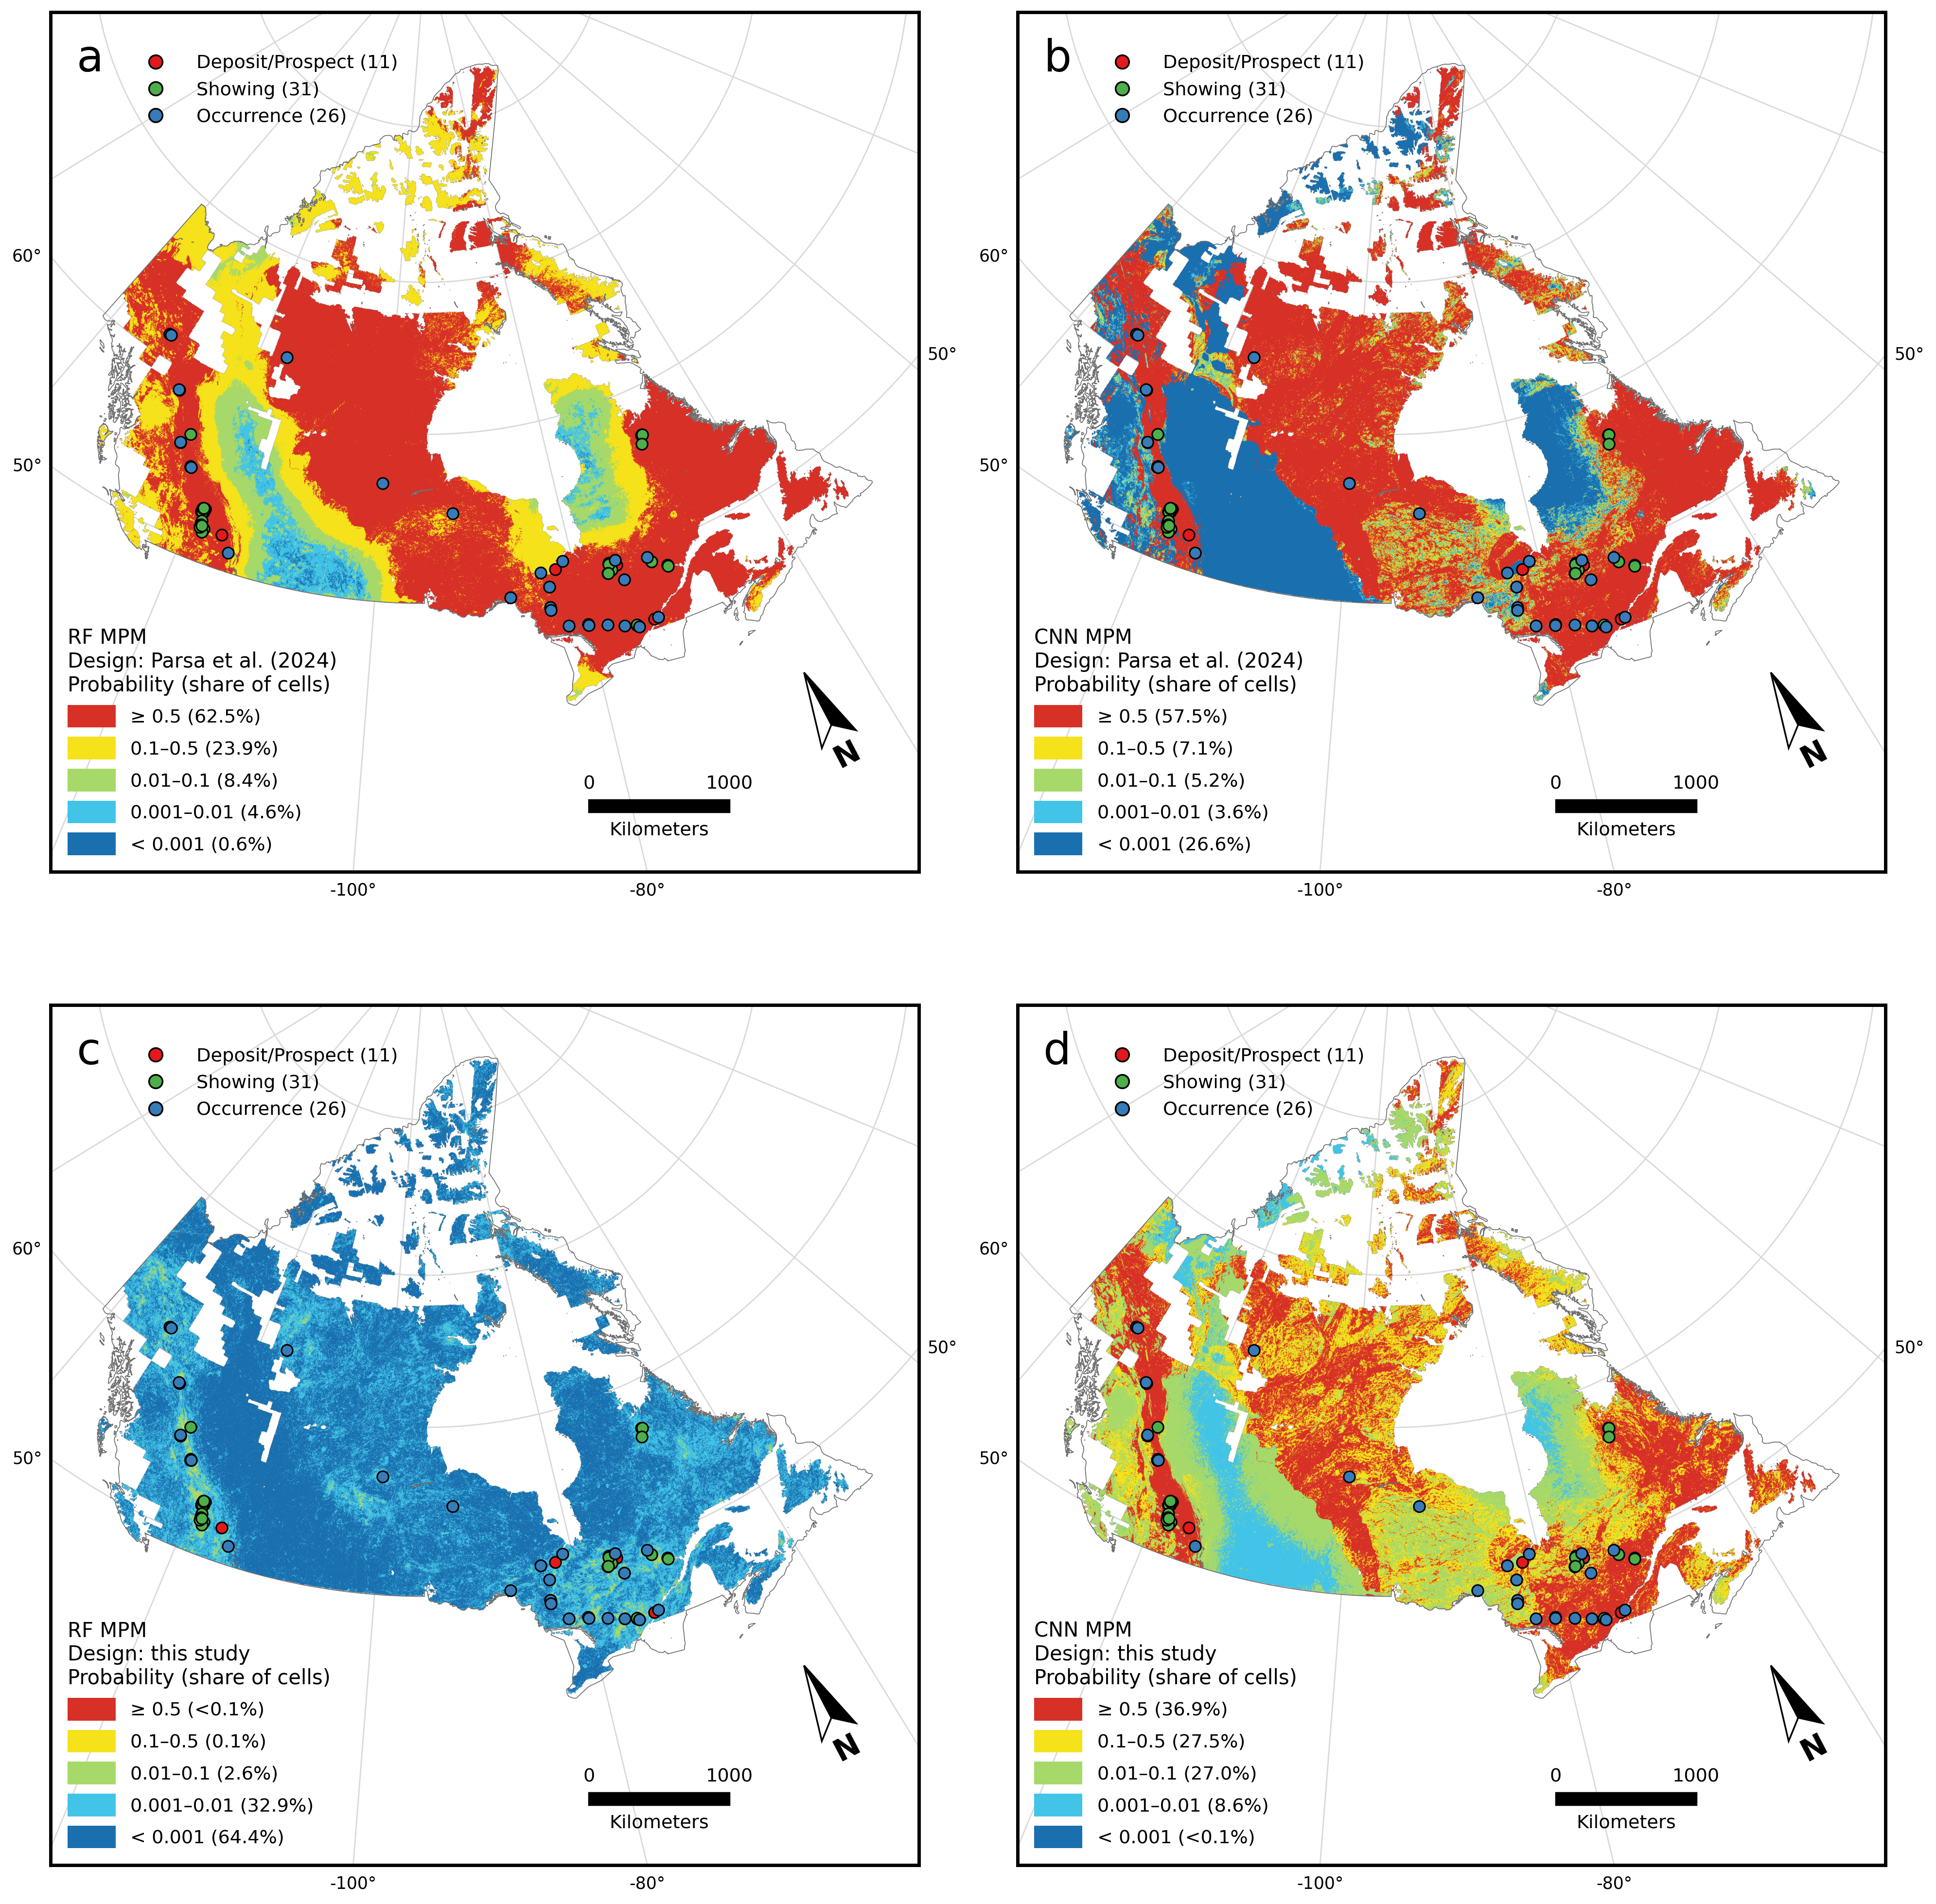
\includegraphics[width=\textwidth]{figures_r7/fig_map_national_logprob_r7.png}
\caption{在表~\ref{tab:nat-design} 的两种设计下，1,616,693 个 S2 第 12 级单元的全国成矿远景，每个模型均用其设计中的全部标签拟合：（a）随机森林和（b）CNN 采用 \citet{Parsa2024} 的设计；（c）随机森林和（d）CNN 采用本文的设计。预测概率的分级在四幅图中相同（括号内为各级单元所占比例）；矿点按开发状态分类（加拿大地图集兰伯特投影）。白色：全国研究区域之外。}\label{fig:nat-maps}
\end{figure}

两种设计得到的地图也截然不同（图~\ref{fig:nat-maps}）。在 \citet{Parsa2024} 的设计下，随机森林对 62.5\% 的单元给出 0.5 及以上的概率，CNN 则为 57.5\%。其负样本取自与矿点最不相似的 5\% 单元，距最近矿点的中位距离为 480~km（全部单元为 355~km），因此只覆盖了输入空间的一个角落：凡是不像这个角落的地方都被归入矿点一类；在 50,000 个随机单元中，61.6\% 的单元其最近的训练样本是正样本。改用 34,761 个随机背景单元后，同一随机森林只对 91 个单元（不到 0.1\%）给出 0.5 及以上的概率，其中 66 个就是矿点单元本身，其余均在距矿点 31~km 以内；而 64.4\% 的单元没有得到其 1,000 棵树中任何一棵的正类投票。此时背景覆盖了整个输入空间，最近训练样本为正样本的随机单元只占 0.2\%，而一棵完全生长的树只有在某个单元与某一矿点非常相似时才会投正类票；概率在 0.01 及以上的 2.8\% 单元距矿点的中位距离为 65~km，其中 79\% 位于科迪勒拉、格伦维尔省和苏必利尔省。采用 \citet{Parsa2024} 的设置、但使用我们的标签和背景时，CNN 缺乏选择性：36.9\% 的单元达到 0.5，10.7\% 达到 0.9，而在其原设计下达到 0.9 的为 48.6\%。它的地图没有突出全国的任何部分，与其对留出矿点的排序（AP 0.059）一样，对找矿靶区圈定几乎不提供信息。两种设计都按平衡的类别比例训练，因此都不给出校准过的概率，这些地图比较的是设计本身，而非成矿概率。但在随机森林和输入都相同的情况下，仅负样本的选取方式就把高概率区从加拿大的大部分地区缩小到已知矿点的紧邻范围。在省级尺度上随机森林的概率同样很低：在苏必利尔省，最终随机森林对 80\% 的预测网格赋予恰好为零的概率（第~\ref{sec:res-maps}~节），因此其地图应按排序而非概率来解读。

全国尺度的比较关注的是标签和负样本如何采样，并不表明应由一个模型覆盖整个国家。加拿大的碳酸岩自约 2.68~Ga 起分多期侵位 \citep{Rukhlov2010}，所处背景各不相同，从太古宙的苏必利尔克拉通到科迪勒拉造山带、格伦维尔造山带以及圣劳伦斯裂谷系 \citep{Groulier2020,Neron2018}，因此同一证据图层不一定在各处代表同一过程：可填图判据的价值取决于它对所代表过程的代表性，而其意义随关键过程发生的尺度而变化 \citep{McCuaig2010}。此外，模型只有在输入与其训练数据相似的地方才是可靠的 \citep{Meyer2021}。因此，我们对苏必利尔省、科迪勒拉和格伦维尔省的矿点分别建模（第~\ref{sec:res-provinces}~节），并用省级模型检验在一个省训练的模型能否用于另一个省（第~\ref{sec:res-transfer}~节）。

\subsection{省级模型}\label{sec:res-provinces}

\subsubsection{随机交叉验证下的模型比较}\label{sec:res-random}

在苏必利尔省，除 nnPU 外的所有模型对留出矿点的排序都远优于随机水平（表~\ref{tab:benchmark}）：AP 为 0.20--0.38（随机排序值为 0.005），AUC 为 0.97--0.99。DevNet 的 AP 中位数最高（0.381），RF 的 AUC 最高（0.985）。在全部六次重复划分中，DevNet 的 AP 均高于 RF、XGBoost（0.265）、bagging-PU 和 nnPU；按各次重复平均后的排序计算，高出 0.18--0.30。与 DevNet 共享网络结构和输入的 nnPU，AP 仅为 0.159，AUC 为 0.842。

对比区域的表现则不同。在科迪勒拉，bagging-PU 和 RF 领先（AP 分别为 0.469 和 0.456），DevNet（0.327；在全部六次重复中均低于 RF）和 XGBoost（0.389）落后。在格伦维尔省，所有模型均较弱；XGBoost 领先（0.368），其次为 RF（0.268），二者在全部六次重复中均优于 DevNet（0.127）。nnPU 在这两个省均失效（AUC 0.58--0.61）。苏必利尔省是三个省中预测效果最好的，这与 \citet{Parsa2024} 的省级成功率一致。

\begin{table}[t]
\caption{汇总的折外 AUC 和 AP（六次重复 5 折随机划分的中位数和 95\% 区间）。粗体：各区域五个模型中的最优值。}\label{tab:benchmark}
\footnotesize
\begin{tabular*}{\textwidth}{@{\extracolsep\fill}llcc}
\toprule
区域（$n_{\mathrm{pos}}$） & 模型 & AUC & AP \\
\midrule
\multirow{5}{*}{苏必利尔省（15）} & DevNet & 0.972 & \textbf{0.381} [0.347, 0.452] \\
 & RF & \textbf{0.985} & 0.268 [0.202, 0.314] \\
 & XGBoost & 0.976 & 0.265 [0.243, 0.298] \\
 & Bagging-PU & 0.976 & 0.198 [0.163, 0.219] \\
 & nnPU & 0.842 & 0.159 [0.096, 0.210] \\
\midrule
\multirow{5}{*}{科迪勒拉（27）} & DevNet & 0.925 & 0.327 [0.263, 0.353] \\
 & RF & 0.936 & 0.456 [0.428, 0.548] \\
 & XGBoost & 0.926 & 0.389 [0.357, 0.448] \\
 & Bagging-PU & \textbf{0.937} & \textbf{0.469} [0.356, 0.485] \\
 & nnPU & 0.575 & 0.023 [0.017, 0.037] \\
\midrule
\multirow{5}{*}{格伦维尔省（12）} & DevNet & 0.826 & 0.127 [0.060, 0.168] \\
 & RF & 0.836 & 0.268 [0.202, 0.320] \\
 & XGBoost & 0.870 & \textbf{0.368} [0.216, 0.429] \\
 & Bagging-PU & \textbf{0.909} & 0.151 [0.133, 0.197] \\
 & nnPU & 0.609 & 0.009 [0.008, 0.010] \\
\botrule
\end{tabular*}
\end{table}

\subsubsection{空间分块交叉验证}\label{sec:res-spatial}

在苏必利尔省，留出整个分块扩大了 DevNet 与基于树的学习器及 PU 学习器之间的差距（图~\ref{fig:spatial}；表~\ref{tab:spatial}）。在 50、100 和 200~km 分块下，DevNet 的 AP 分别为 0.371、0.345 和 0.221。RF 的 AP 从随机划分下的 0.268 降至 0.165、0.129 和 0.087，XGBoost 从 0.265 降至 0.177、0.119 和 0.098，bagging-PU 降至 0.133、0.076 和 0.072。在每种分块大小下，DevNet 在全部六次重复中的 AP 均高于 RF、XGBoost 和 bagging-PU，并在 18 次中的 16 次高于 nnPU；相对 RF 高出 $+0.23$ 至 $+0.31$，相对 XGBoost 高出 $+0.21$ 至 $+0.33$，相对 bagging-PU 高出 $+0.25$ 至 $+0.39$，相对 nnPU 高出 $+0.13$ 至 $+0.30$。然而，由于只有 15 个矿点，与 RF 之差的 95\% 区间下限低至 0.03--0.06，因此相对 RF 的优势是一致的，但其大小并不确定。各模型之间 AUC 的差异较小（附录~\ref{app:full}，表~\ref{tab:spatial-auc}）：在 50~km 分块下 RF 的 AUC 最高（0.976，DevNet 为 0.969），在 100 和 200~km 分块下 DevNet 最高（0.928 和 0.886）。在 50 和 100~km 分块下，DevNet 排序最低的矿点是位于 KSZ 上的 Kapuskasing 和 Nemegosenda Lake。

捕获率曲线（图~\ref{fig:capture}）显示了 AP 差异产生于何处。在随机划分下，DevNet 和 RF 在排序样本池的前 1\% 中捕获了约一半的留出矿点（53\% 和 50\%）；到前 10\% 时，RF 捕获了全部矿点，bagging-PU 捕获 97\%，DevNet 捕获 93\%。在 50 和 100~km 分块下，DevNet 保持了其前 1\% 捕获率的大部分（53\% 和 43\%），到前 10\% 时捕获 93\% 和 87\%；而 RF 在前 1\% 中捕获 40\% 和 27\%（到前 10\% 时为 100\% 和 77\%），bagging-PU 为 30\% 和 23\%（90\% 和 70\%）。在 200~km 分块下，每个模型在前 1\% 中的捕获率均不超过 40\%；到前 10\% 时，DevNet 和 bagging-PU（70\%）略高于 RF（63\%）。

在科迪勒拉，所有模型在分块下均急剧退化（50~km 时 AP $\leq 0.13$，100--200~km 时 $\leq 0.07$）；在格伦维尔省，AP 接近随机排序值（100--200~km 时 $\leq 0.010$）。在这些区域中，模型间的任何差异都不具有实际意义的大小：它们在随机划分下的预测能力在很大程度上归因于训练矿点与测试矿点之间的空间邻近性（第~\ref{sec:disc-provinces}~节）。

\begin{figure}[t]
\centering
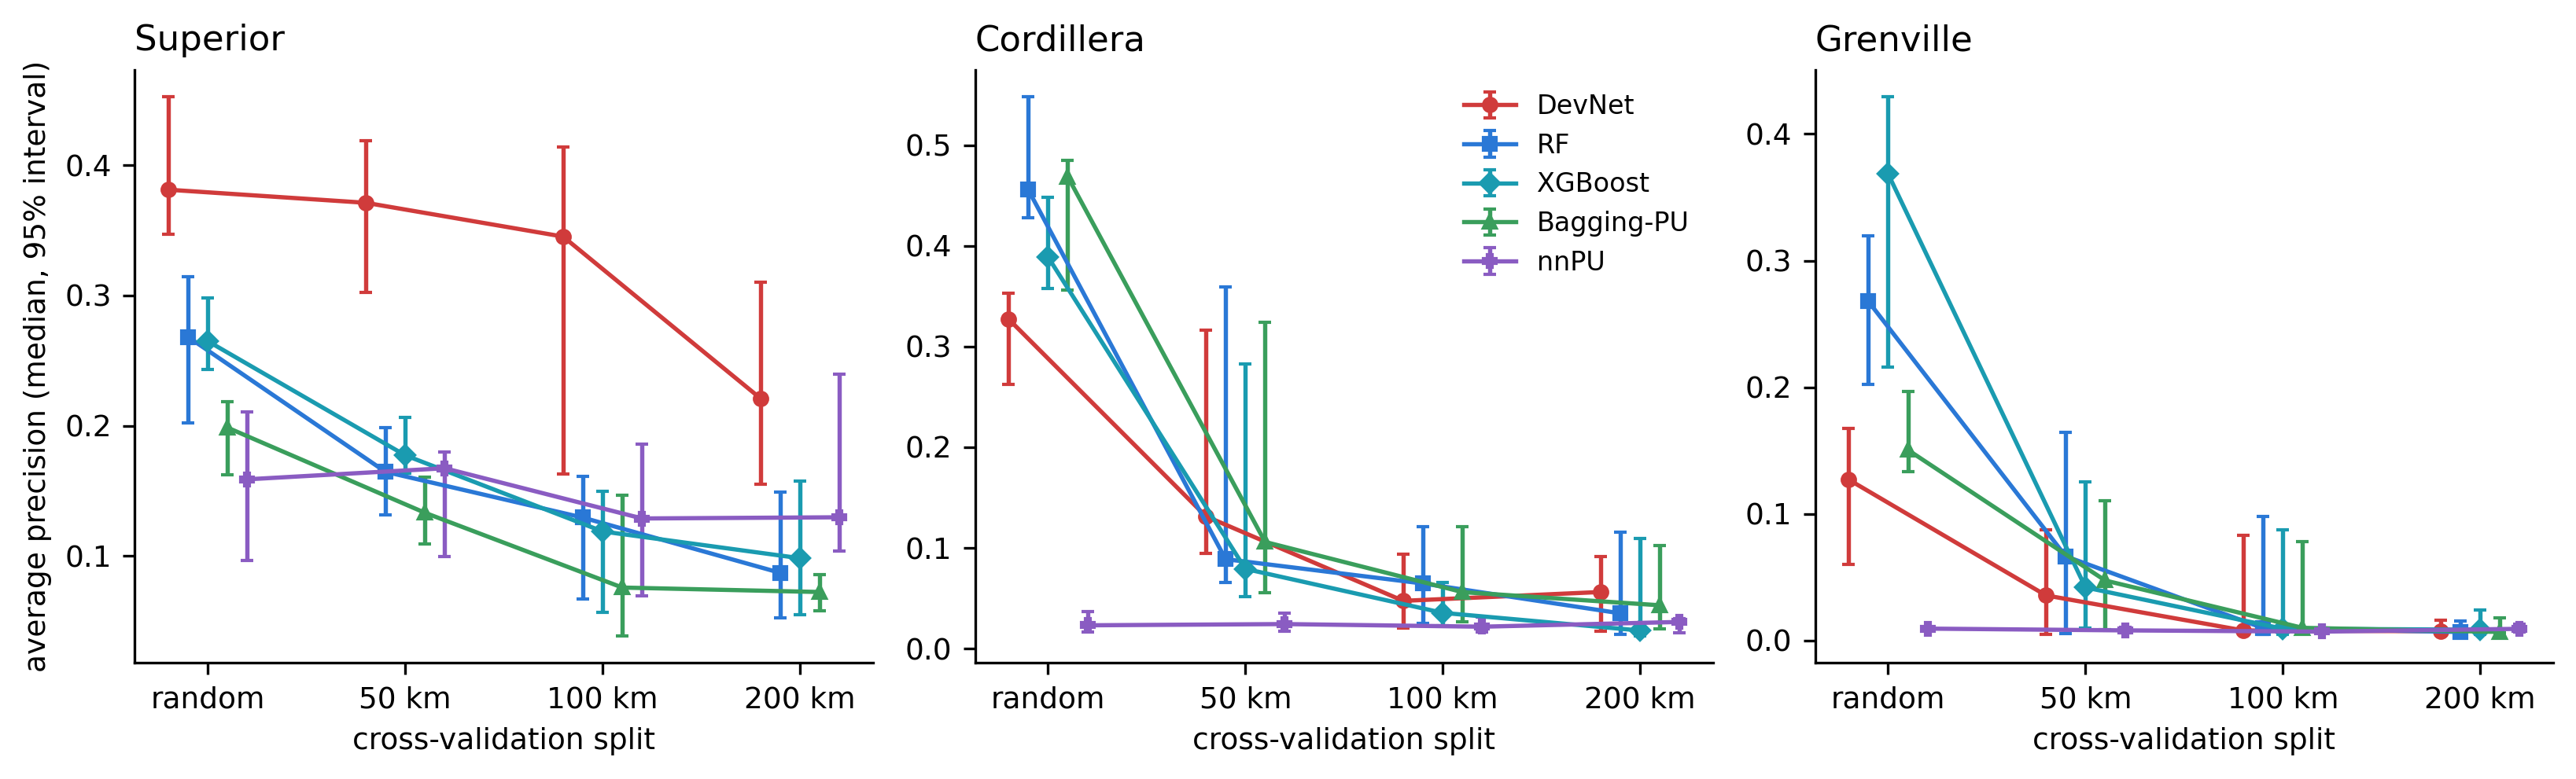
\includegraphics[width=\textwidth]{figures_r7/fig_spatial_cv_r5.png}
\caption{随机交叉验证与空间分块交叉验证下的平均精度（六次重复的中位数和 95\% 区间）。随机排序的 AP 为 0.005（苏必利尔省）、0.009（科迪勒拉）和 0.004（格伦维尔省）。}\label{fig:spatial}
\end{figure}

\begin{figure}[t]
\centering
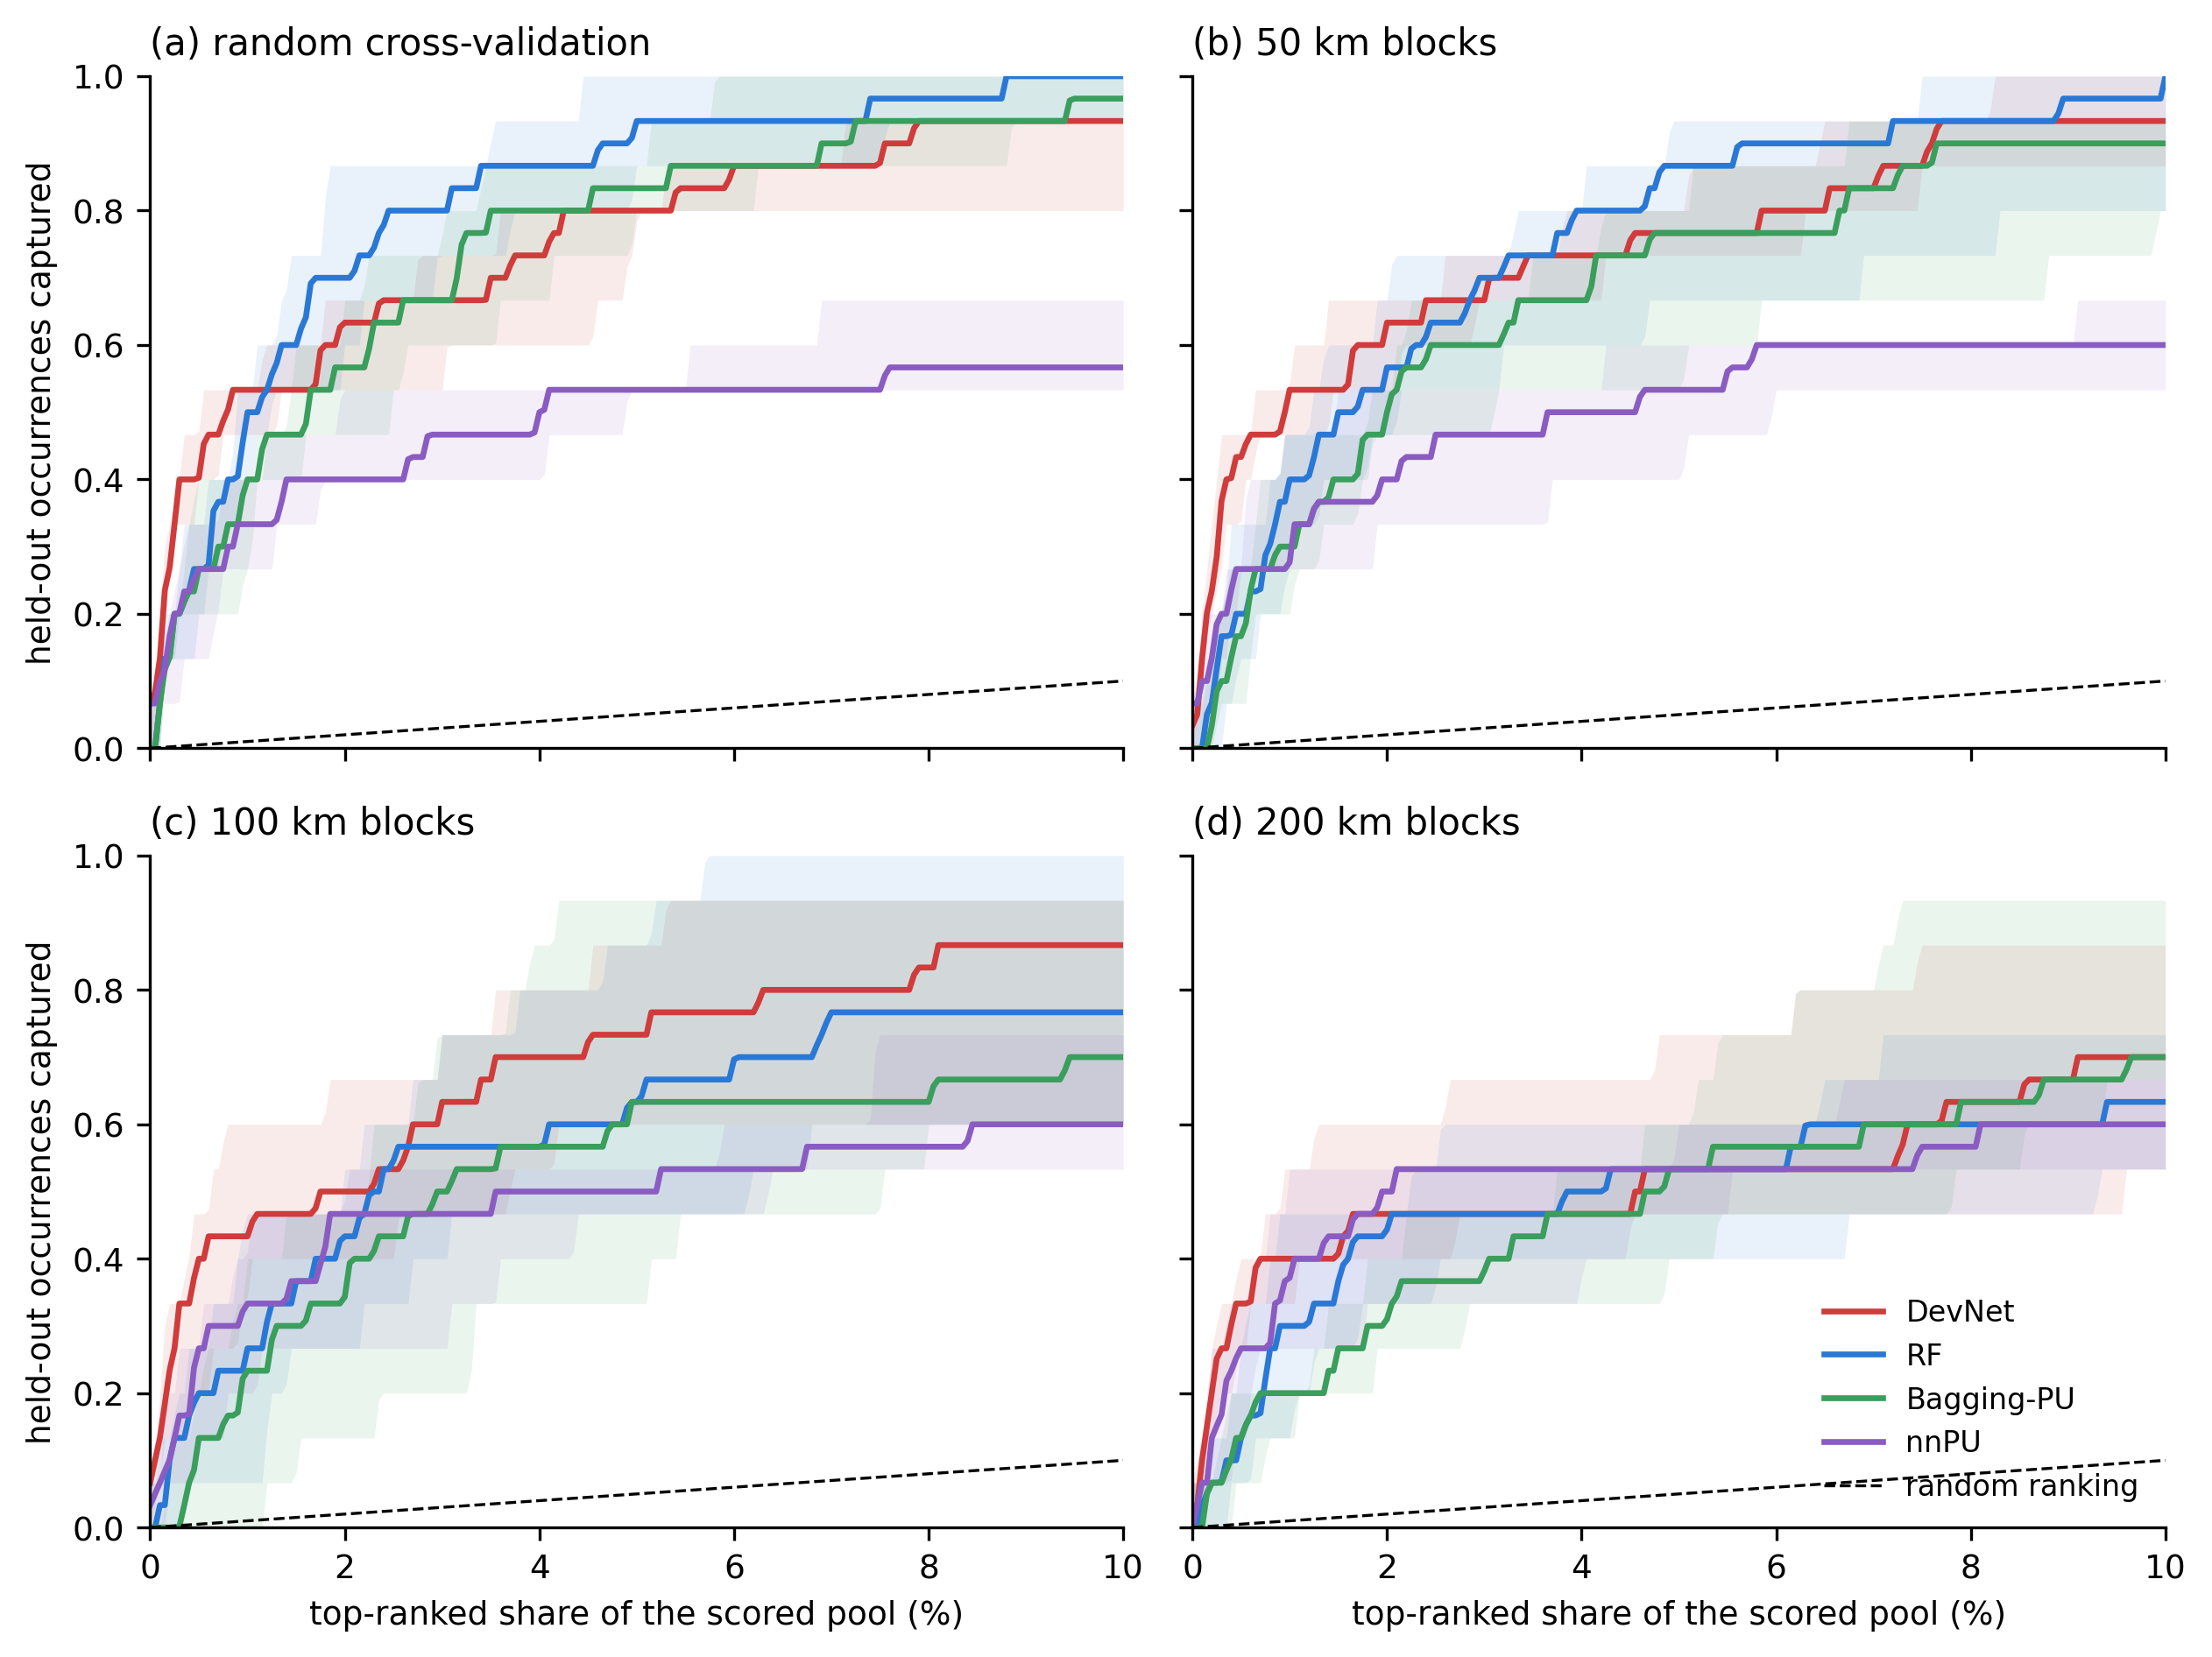
\includegraphics[width=0.92\textwidth]{figures_r7/fig_capture_superior_r4.png}
\caption{苏必利尔省捕获率曲线：在（a）随机交叉验证以及（b）50~km、（c）100~km 和（d）200~km 空间分块下，排在评分样本池前若干比例（作为搜索面积的代理指标）之内的留出矿点所占比例。曲线：六次重复的中位数；色带：范围。虚线：随机排序。}\label{fig:capture}
\end{figure}

\begin{table}[t]
\caption{随机交叉验证与空间分块交叉验证下的平均精度（六次重复的中位数）。粗体：每行最高的 AP。相同运行的 AUC 见附录~\ref{app:full}（表~\ref{tab:spatial-auc}）。}\label{tab:spatial}
\footnotesize
\setlength{\tabcolsep}{3pt}
\begin{tabular*}{\textwidth}{@{\extracolsep\fill}llccccc}
\toprule
区域 & 划分 & DevNet & RF & XGBoost & Bagging-PU & nnPU \\
\midrule
\multirow{4}{*}{苏必利尔省} & 随机 & \textbf{0.381} & 0.268 & 0.265 & 0.198 & 0.159 \\
 & 50 km & \textbf{0.371} & 0.165 & 0.177 & 0.133 & 0.167 \\
 & 100 km & \textbf{0.345} & 0.129 & 0.119 & 0.076 & 0.129 \\
 & 200 km & \textbf{0.221} & 0.087 & 0.098 & 0.072 & 0.130 \\
\midrule
\multirow{4}{*}{科迪勒拉} & 随机 & 0.327 & 0.456 & 0.389 & \textbf{0.469} & 0.023 \\
 & 50 km & \textbf{0.131} & 0.089 & 0.079 & 0.106 & 0.024 \\
 & 100 km & 0.048 & \textbf{0.065} & 0.036 & 0.056 & 0.022 \\
 & 200 km & \textbf{0.056} & 0.035 & 0.018 & 0.043 & 0.027 \\
\midrule
\multirow{4}{*}{格伦维尔省} & 随机 & 0.127 & 0.268 & \textbf{0.368} & 0.151 & 0.009 \\
 & 50 km & 0.036 & \textbf{0.067} & 0.042 & 0.047 & 0.008 \\
 & 100 km & 0.008 & 0.010 & 0.009 & \textbf{0.010} & 0.007 \\
 & 200 km & 0.007 & 0.007 & 0.009 & 0.007 & \textbf{0.009} \\
\botrule
\end{tabular*}
\end{table}

\subsubsection{地质图类别的贡献}\label{sec:res-featuresets}

在苏必利尔省，单一地质图类别承载了很大一部分预测能力。去除碱性侵入体这一列后，在随机划分以及 50、100 和 200~km 分块下，DevNet 的 AP 降至 0.346、0.260、0.177 和 0.137，RF 降至 0.194、0.126、0.065 和 0.067：这一个类别覆盖了苏必利尔省 15 个矿点中的 6 个以及 0.5\% 的背景，贡献了 DevNet 空间分块 AP 的 30--49\%。在每种分块大小下，去除该类别的 DevNet 的 AP 仍高于保留该类别的 RF。去除所有点位级地质图类别会使 DevNet 和 RF 损失约一半或更多的 AP：DevNet 的 AP 在随机划分下降至 0.159，在分块下降至 0.123、0.081 和 0.075；RF 分别降至 0.146 以及 0.084、0.044 和 0.050。在没有地质图类别的情况下，DevNet 在每种分块大小下仍具有最高的 AP，领先于 XGBoost（0.105、0.050 和 0.062）和 bagging-PU（0.102、0.058 和 0.066）；而在随机划分下 XGBoost 和 bagging-PU 领先（0.175 和 0.174），nnPU 失效（AP 0.009）。

\subsubsection{正样本增强}\label{sec:res-augmentation}

各生成器的表现差异很大（表~\ref{tab:aug-diag}；附录~\ref{app:aug-spatial}，图~\ref{fig:aug-pca}）。抖动和 SMOTE 样本紧邻真实正样本（最近邻距离比中位数为 0.11 和 0.24），且几乎全部以真实正样本作为其最近的有标签邻居（100\% 和 99\%）：它们几乎是训练矿点的副本。WGAN-GP 样本与真实正样本之间的距离，和真实正样本彼此之间的距离相当（比值 0.97），但其中 37\% 的最近有标签点是背景点：在只有 15 个训练点的情况下，生成器将概率质量扩散到了特征空间中类似背景的区域。三组样本均获得较高的 DevNet 得分（百分位中位数为 0.98）。

有无增强时所用的折完全相同（表~\ref{tab:augmentation}；图~\ref{fig:aug-perf}）。对 DevNet 而言，每种生成器都使 AP 中位数有所提高（增强后其 AP 介于 0.408 与 0.432 之间，未增强时为 0.381），但并不稳定：在六次重复划分中，增强后的 DevNet 仅在两到五次中 AP 更高。对 RF 而言，抖动使 AP 从 0.268 变为 0.264--0.310，SMOTE 使其降低（0.198--0.236），WGAN-GP 使其提高（0.278--0.327）。最佳的增强 RF（WGAN-GP $10\times$，AP 0.327）仍低于未增强的 DevNet（0.381）。在空间分块下（附录~\ref{app:aug-spatial}，表~\ref{tab:aug-spatial}），WGAN-GP 将 RF 在 100~km 分块下的 AP 从 0.129 提高到 0.135--0.191，在 200~km 分块下从 0.087 提高到 0.122--0.132，但仍远低于未增强的 DevNet（0.345 和 0.221）；而抖动和 SMOTE 对其影响很小（0.110--0.139 和 0.077--0.096）。DevNet 的 AP 在 100~km 分块下变化很小（0.308--0.341，对照为 0.343），在 200~km 分块下在 0.200 与 0.258 之间变动（对照为 0.216）。

\begin{figure}[t]
\centering
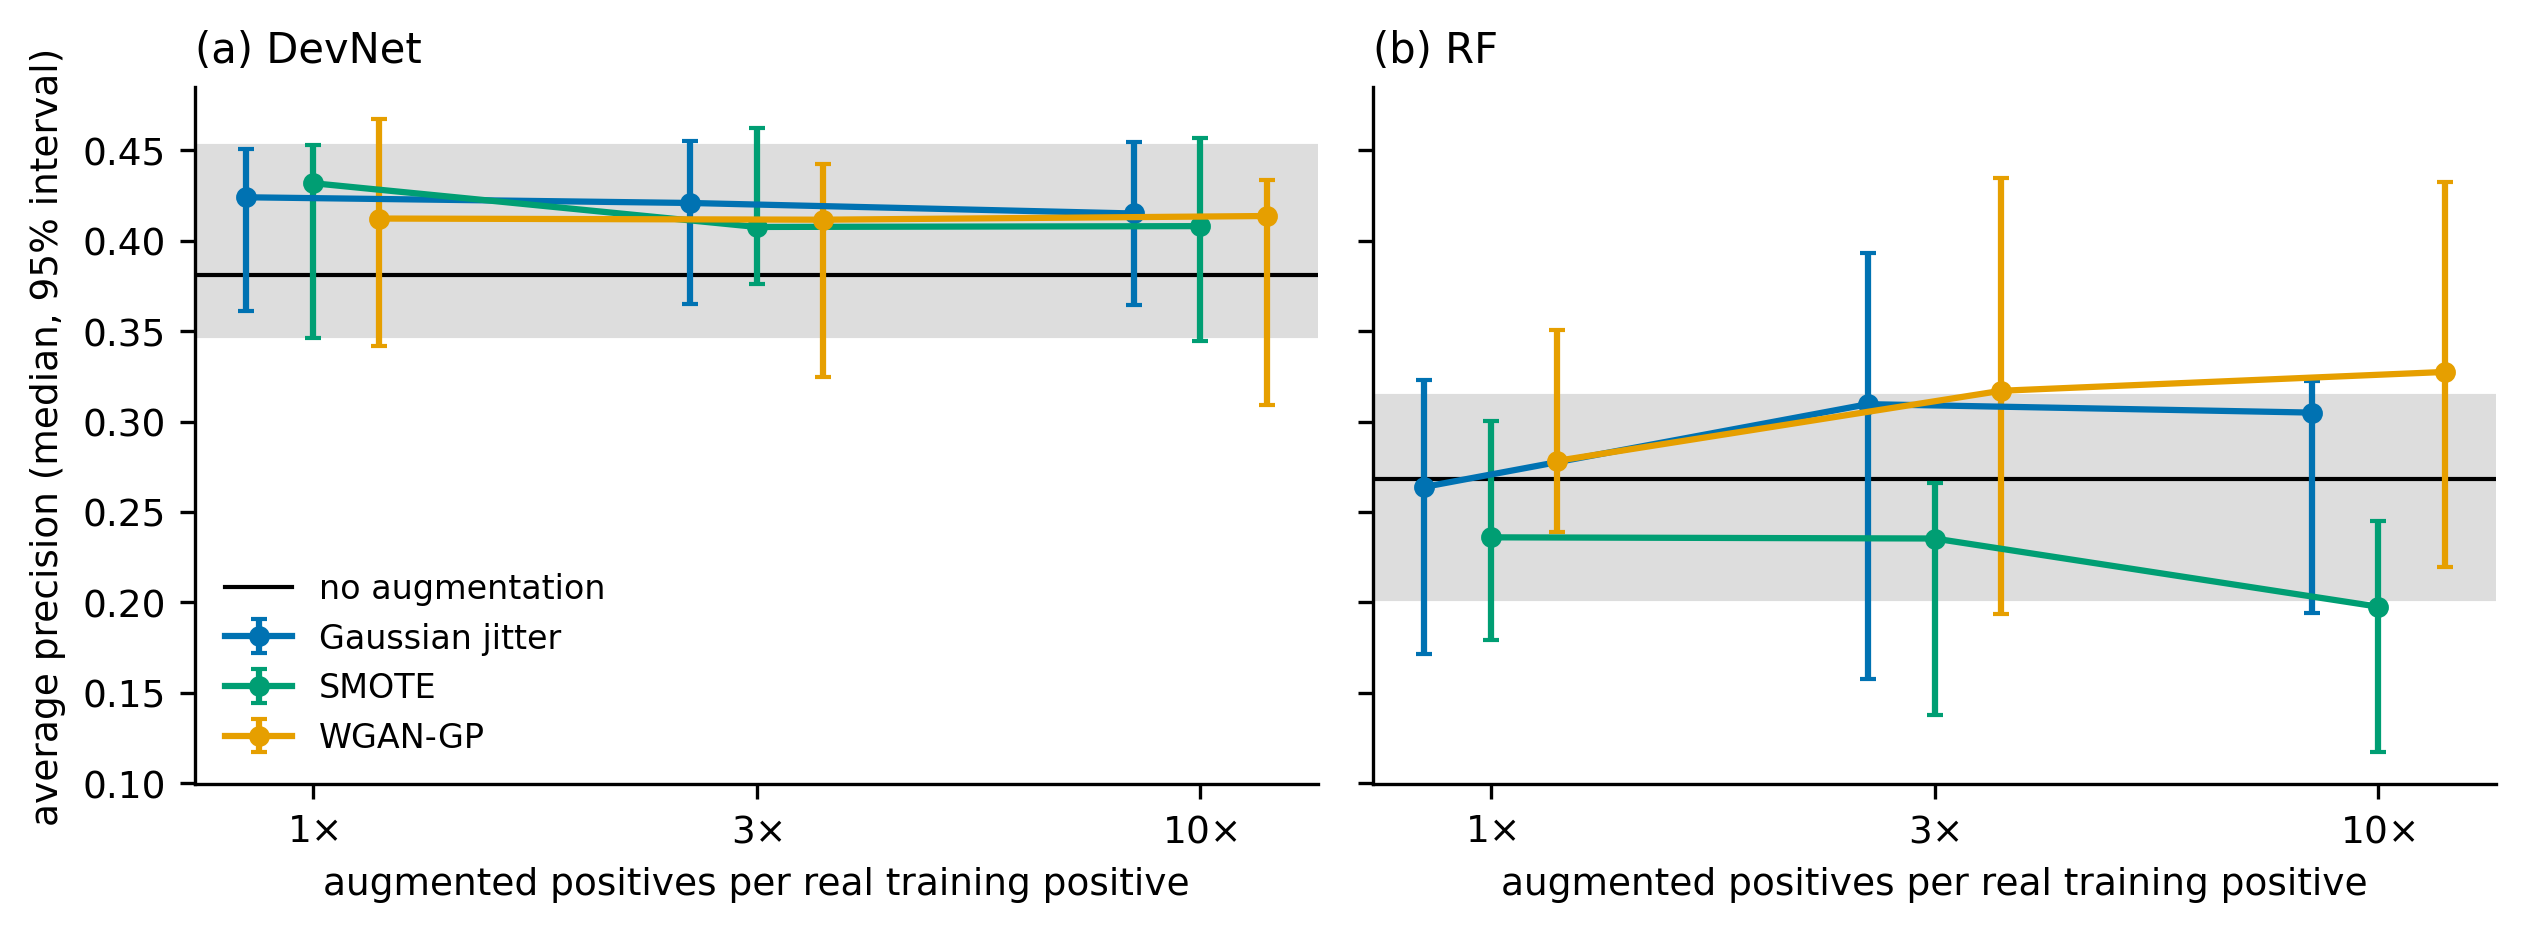
\includegraphics[width=\textwidth]{figures_r7/fig_augmentation_performance_r4.png}
\caption{苏必利尔省采用折内安全（fold-safe）正样本增强时的平均精度，按生成器及每个真实训练正样本对应的增强正样本数量分列。直线与灰色条带：无增强（中位数和 95\% 区间）。}\label{fig:aug-perf}
\end{figure}

\begin{table}[t]
\caption{苏必利尔省的折内安全正样本增强（随机交叉验证，折完全相同；留出正样本始终为真实样本）：AUC 和 AP（六次重复的中位数和 95\% 区间）。}\label{tab:augmentation}
\footnotesize
\begin{tabular*}{0.8\textwidth}{@{\extracolsep\fill}lllcc}
\toprule
模型 & 生成器 & $m$ & AUC & AP \\
\midrule
\multirow{10}{*}{DevNet} & 无 & -- & 0.972 & 0.381 [0.347, 0.452] \\
 & 高斯抖动 & 1$\times$ & 0.966 & 0.424 [0.361, 0.451] \\
 & 高斯抖动 & 3$\times$ & 0.969 & 0.421 [0.365, 0.455] \\
 & 高斯抖动 & 10$\times$ & 0.971 & 0.415 [0.364, 0.455] \\
 & SMOTE & 1$\times$ & 0.973 & 0.432 [0.346, 0.453] \\
 & SMOTE & 3$\times$ & 0.975 & 0.408 [0.376, 0.462] \\
 & SMOTE & 10$\times$ & 0.970 & 0.408 [0.344, 0.457] \\
 & WGAN-GP & 1$\times$ & 0.973 & 0.412 [0.342, 0.467] \\
 & WGAN-GP & 3$\times$ & 0.968 & 0.412 [0.325, 0.442] \\
 & WGAN-GP & 10$\times$ & 0.960 & 0.414 [0.309, 0.433] \\
\midrule
\multirow{10}{*}{RF} & 无 & -- & 0.985 & 0.268 [0.202, 0.314] \\
 & 高斯抖动 & 1$\times$ & 0.964 & 0.264 [0.171, 0.323] \\
 & 高斯抖动 & 3$\times$ & 0.983 & 0.310 [0.158, 0.393] \\
 & 高斯抖动 & 10$\times$ & 0.980 & 0.305 [0.194, 0.323] \\
 & SMOTE & 1$\times$ & 0.981 & 0.236 [0.179, 0.300] \\
 & SMOTE & 3$\times$ & 0.983 & 0.235 [0.138, 0.266] \\
 & SMOTE & 10$\times$ & 0.980 & 0.198 [0.117, 0.245] \\
 & WGAN-GP & 1$\times$ & 0.984 & 0.278 [0.239, 0.351] \\
 & WGAN-GP & 3$\times$ & 0.983 & 0.317 [0.193, 0.435] \\
 & WGAN-GP & 10$\times$ & 0.984 & 0.327 [0.219, 0.433] \\
\botrule
\end{tabular*}
\end{table}

\begin{table}[t]
\caption{各生成器的产出（拟合于苏必利尔省全部 15 个正样本；每种 150 个样本）。最近邻距离比：到最近真实正样本的距离除以真实正样本之间最近邻距离的中位数（0 = 副本）。最近有标签邻居：在正样本和训练背景中，最近点为正样本的样本所占比例。DevNet 百分位：在最终（生产）DevNet 下，得分在训练背景中所处百分位的中位数。}\label{tab:aug-diag}
\footnotesize
\setlength{\tabcolsep}{2.5pt}
\begin{tabular*}{\textwidth}{@{\extracolsep\fill}lcccc}
\toprule
来源 & 最近邻距离比，中位数 & 最近邻距离比，P10 & 最近邻为正样本 & DevNet 百分位 \\
\midrule
真实矿点（留一法） & 1.00 & 0.60 & -- & 0.996 \\
高斯抖动 & 0.11 & 0.09 & 100\% & 0.985 \\
SMOTE & 0.24 & 0.07 & 99\% & 0.983 \\
WGAN-GP & 0.97 & 0.65 & 63\% & 0.983 \\
背景（300 个随机点） & 1.53 & -- & -- & 0.500 \\
\botrule
\end{tabular*}
\end{table}

\subsubsection{省际迁移能力}\label{sec:res-transfer}

一个省的模型无法预测另一个省（图~\ref{fig:transfer}）。在各省内部，随机交叉验证给出的 AP 为 0.13--0.47（不含 nnPU）；应用于另一省时，树集成模型仅达到 0.004--0.016，约等于随机排序值 0.004--0.009，并且在 30 个模型-省份组合中有 18 个的 AUC 低于 0.5：模型将另一省的矿点排在其背景之下。例外情况是在科迪勒拉训练的 DevNet、XGBoost 和 nnPU 以及在格伦维尔省训练的 bagging-PU 应用于苏必利尔省时：它们的 AUC 达到 0.73--0.75，但 AP 仅为 0.013--0.086，而随机排序为 0.005。从全国模型中留出一个省也得到同样的结果：被留出的格伦维尔省的排序接近随机水平（AUC 0.36--0.67，AP $\leq 0.037$，随机排序为 0.004），被留出的苏必利尔省的 AP 最高仅为 0.051（随机排序为 0.005）。

在输入空间中，各省是彼此不同的域。随机森林区分任意两个省份组训练背景的 AUC 为 0.999--1.000，区分苏必利尔省、科迪勒拉和格伦维尔省彼此之间矿点的 AUC 为 0.99--1.00。若干输入在不同省份中以相反的方向指示矿点。单独来看，LAB 深度区分苏必利尔省矿点与其背景的 AUC 为 0.22（矿点处 LAB 较浅），而对科迪勒拉矿点则为 0.67（较深）；莫霍面深度分别为 0.35 和 0.78，到区域绿岩的距离分别为 0.23 和 0.63；深源磁异常对科迪勒拉和格伦维尔省矿点的指示方向相反（0.25 和 0.81）。这证实了各省必须分别建模。

\begin{figure}[t]
\centering
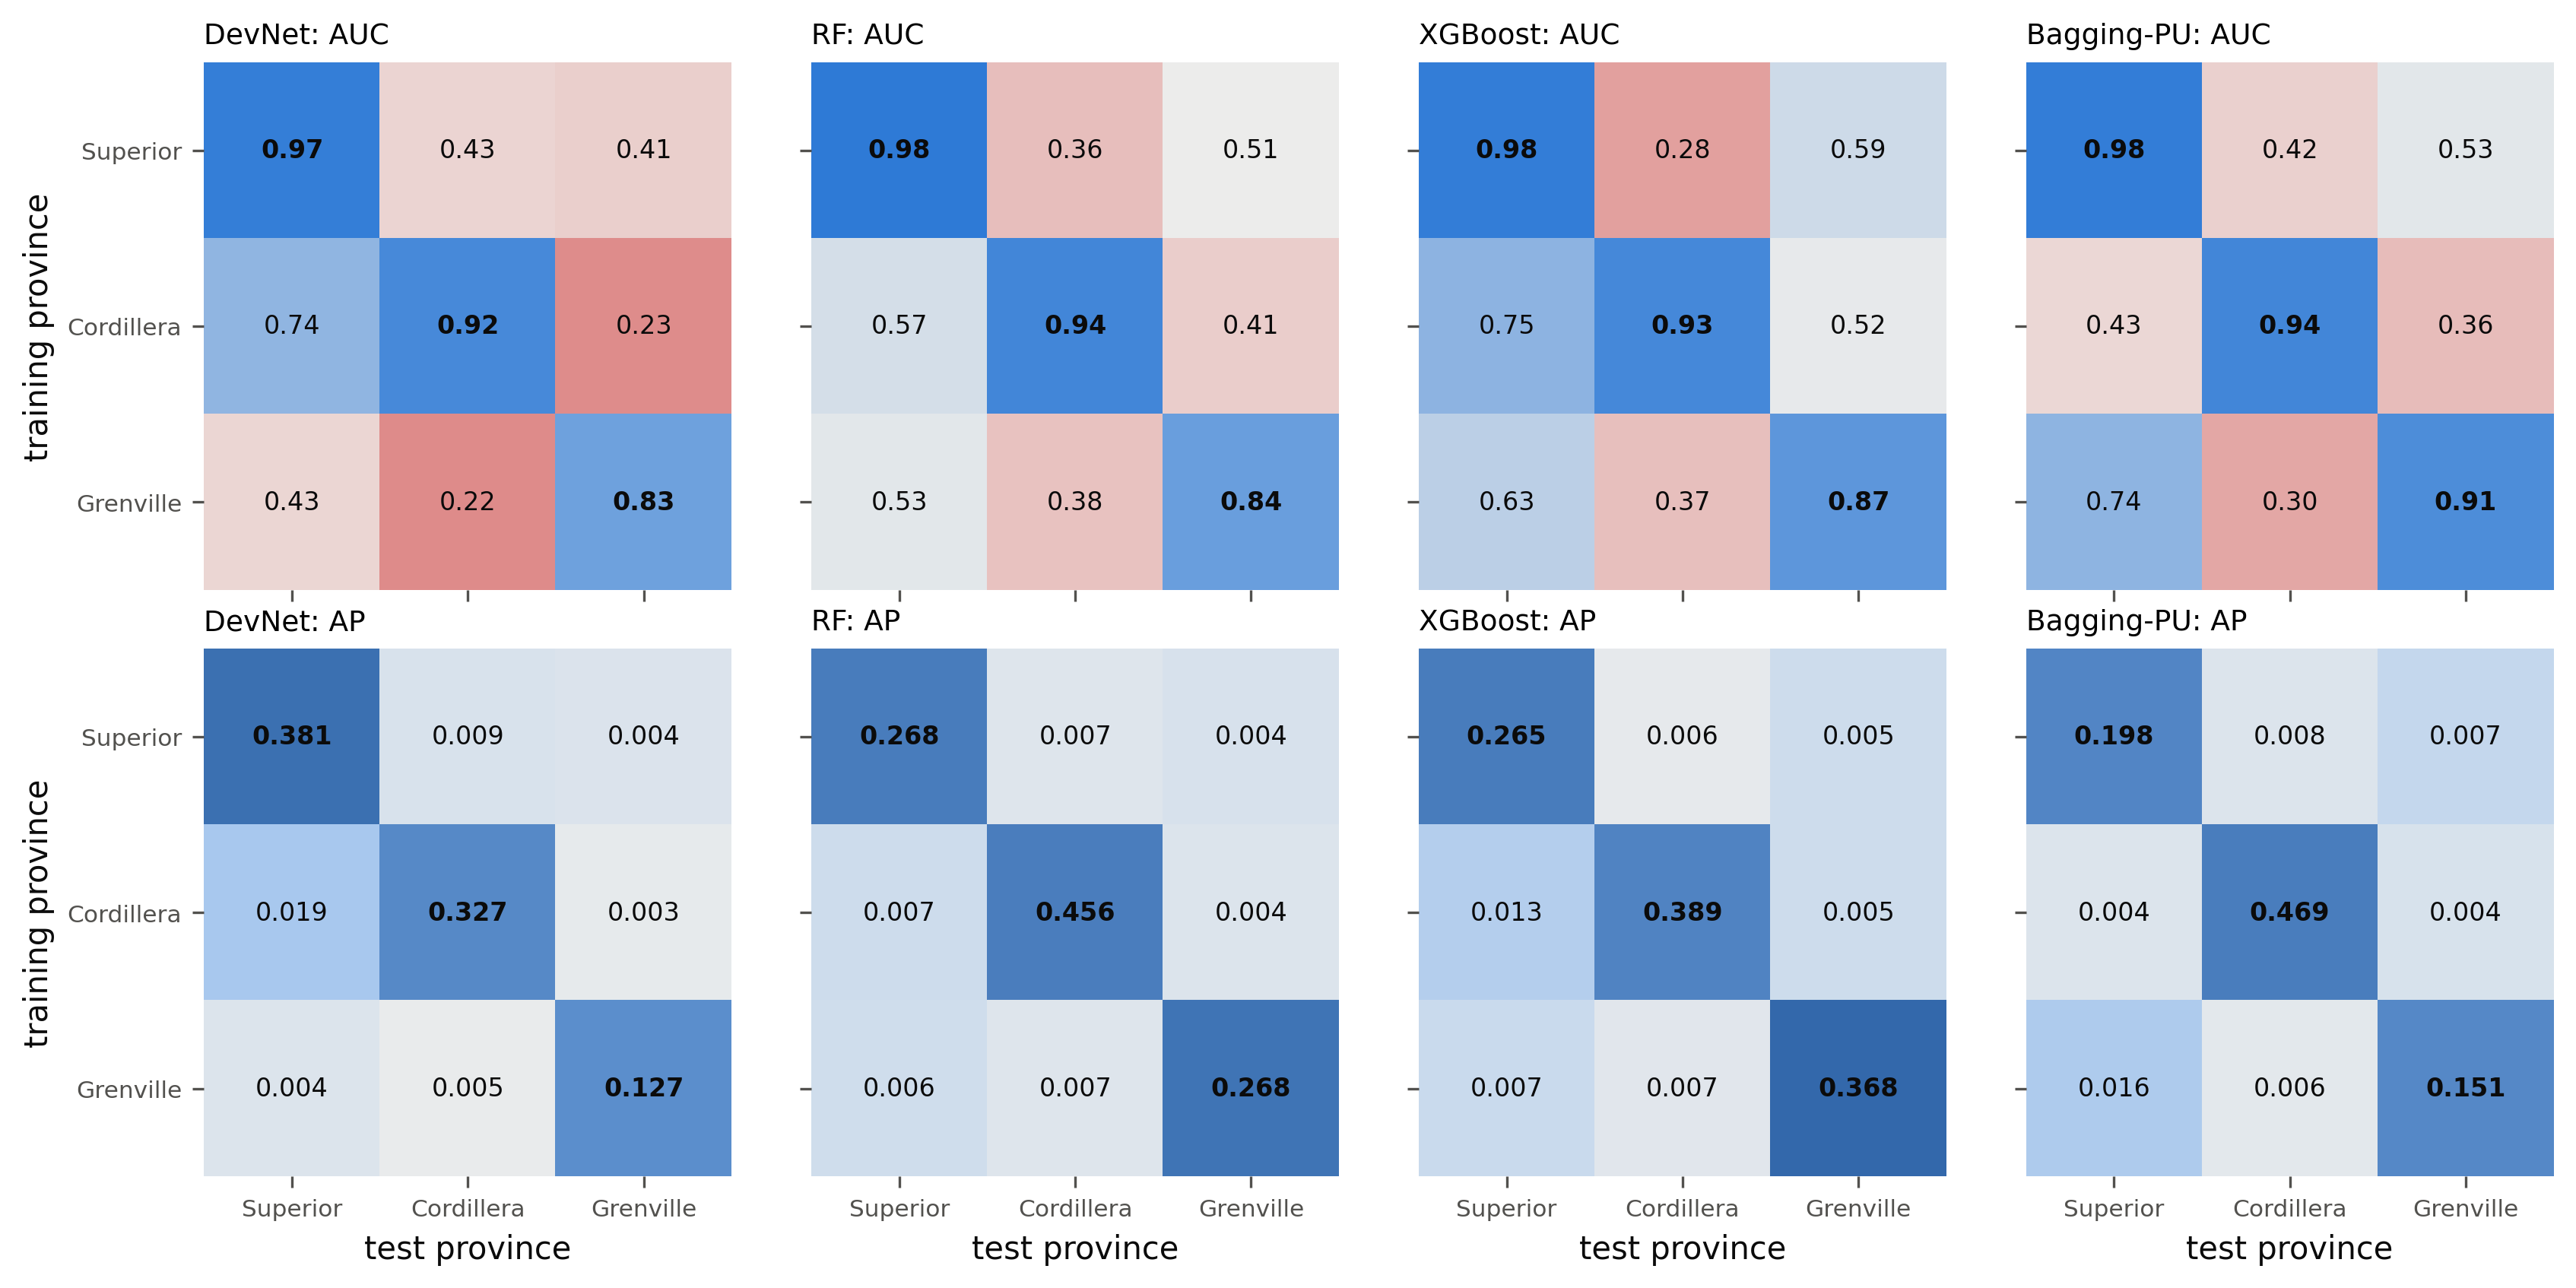
\includegraphics[width=\textwidth]{figures_r7/fig_transfer_r5.png}
\caption{省际迁移。上：AUC；下：AP，颜色表示 AP 除以测试省份的正样本比例（对数刻度）。行：所应用模型（输入、容量、矿点、训练背景）所属的省份；列：被评分的矿点及评估背景所属的省份（六个随机种子的中位数）。对角线为省内随机交叉验证（表~\ref{tab:benchmark}）。}\label{fig:transfer}
\end{figure}

\subsubsection{模型解释}\label{sec:res-shap}

采用基于秩的方向判定规则时，在每个省中，RF 与 DevNet 对二者共同最重要的全部十个特征的效应符号都一致（表~\ref{tab:shap}；附录~\ref{app:shap}）。若改为依据平均 SHAP 值的符号来判读，两个模型会在其中许多特征上显得不一致，这是两种解释器基线不同所造成的假象（第~\ref{sec:shap}~节）。

两个模型在方向上一致，但对证据的权重不同（图~\ref{fig:shap}）。在苏必利尔省，DevNet 将单元的五个地质类别排在最前：喷出岩（绿岩）岩性、单元内的年代接触带和碱性侵入岩岩性提高得分，太古宙和英云闪长岩降低得分；其后为与区域绿岩的邻近度、LAB 深度和布格重力异常 GLCM 相关性（值越低越有远景）。RF 将深源磁异常的水平梯度模排在首位（值越低越有远景），其后为 LAB 深度、与区域绿岩的邻近度、断层邻近度和化极磁异常的一阶垂向导数，而地质类别排名靠后（57 个中的第 22--41 位）。两个模型都认为 LAB 较浅、靠近绿岩带和断层、TMI 较高以及远离深部磁力蠕虫的区域更有远景。在科迪勒拉，两个模型都将中生代地体和远离高级变质单元的区域视为不利，而将元古宙地体视为有利。在格伦维尔省，两个模型都将深源磁异常和布格重力异常 THD 倾斜角的 GLCM 对比度列入其五个最重要特征之中，但鉴于该区预测能力较弱，这些归因描述的是模型试图利用的信号，而非可靠的控矿因素。

\begin{figure}[t]
\centering
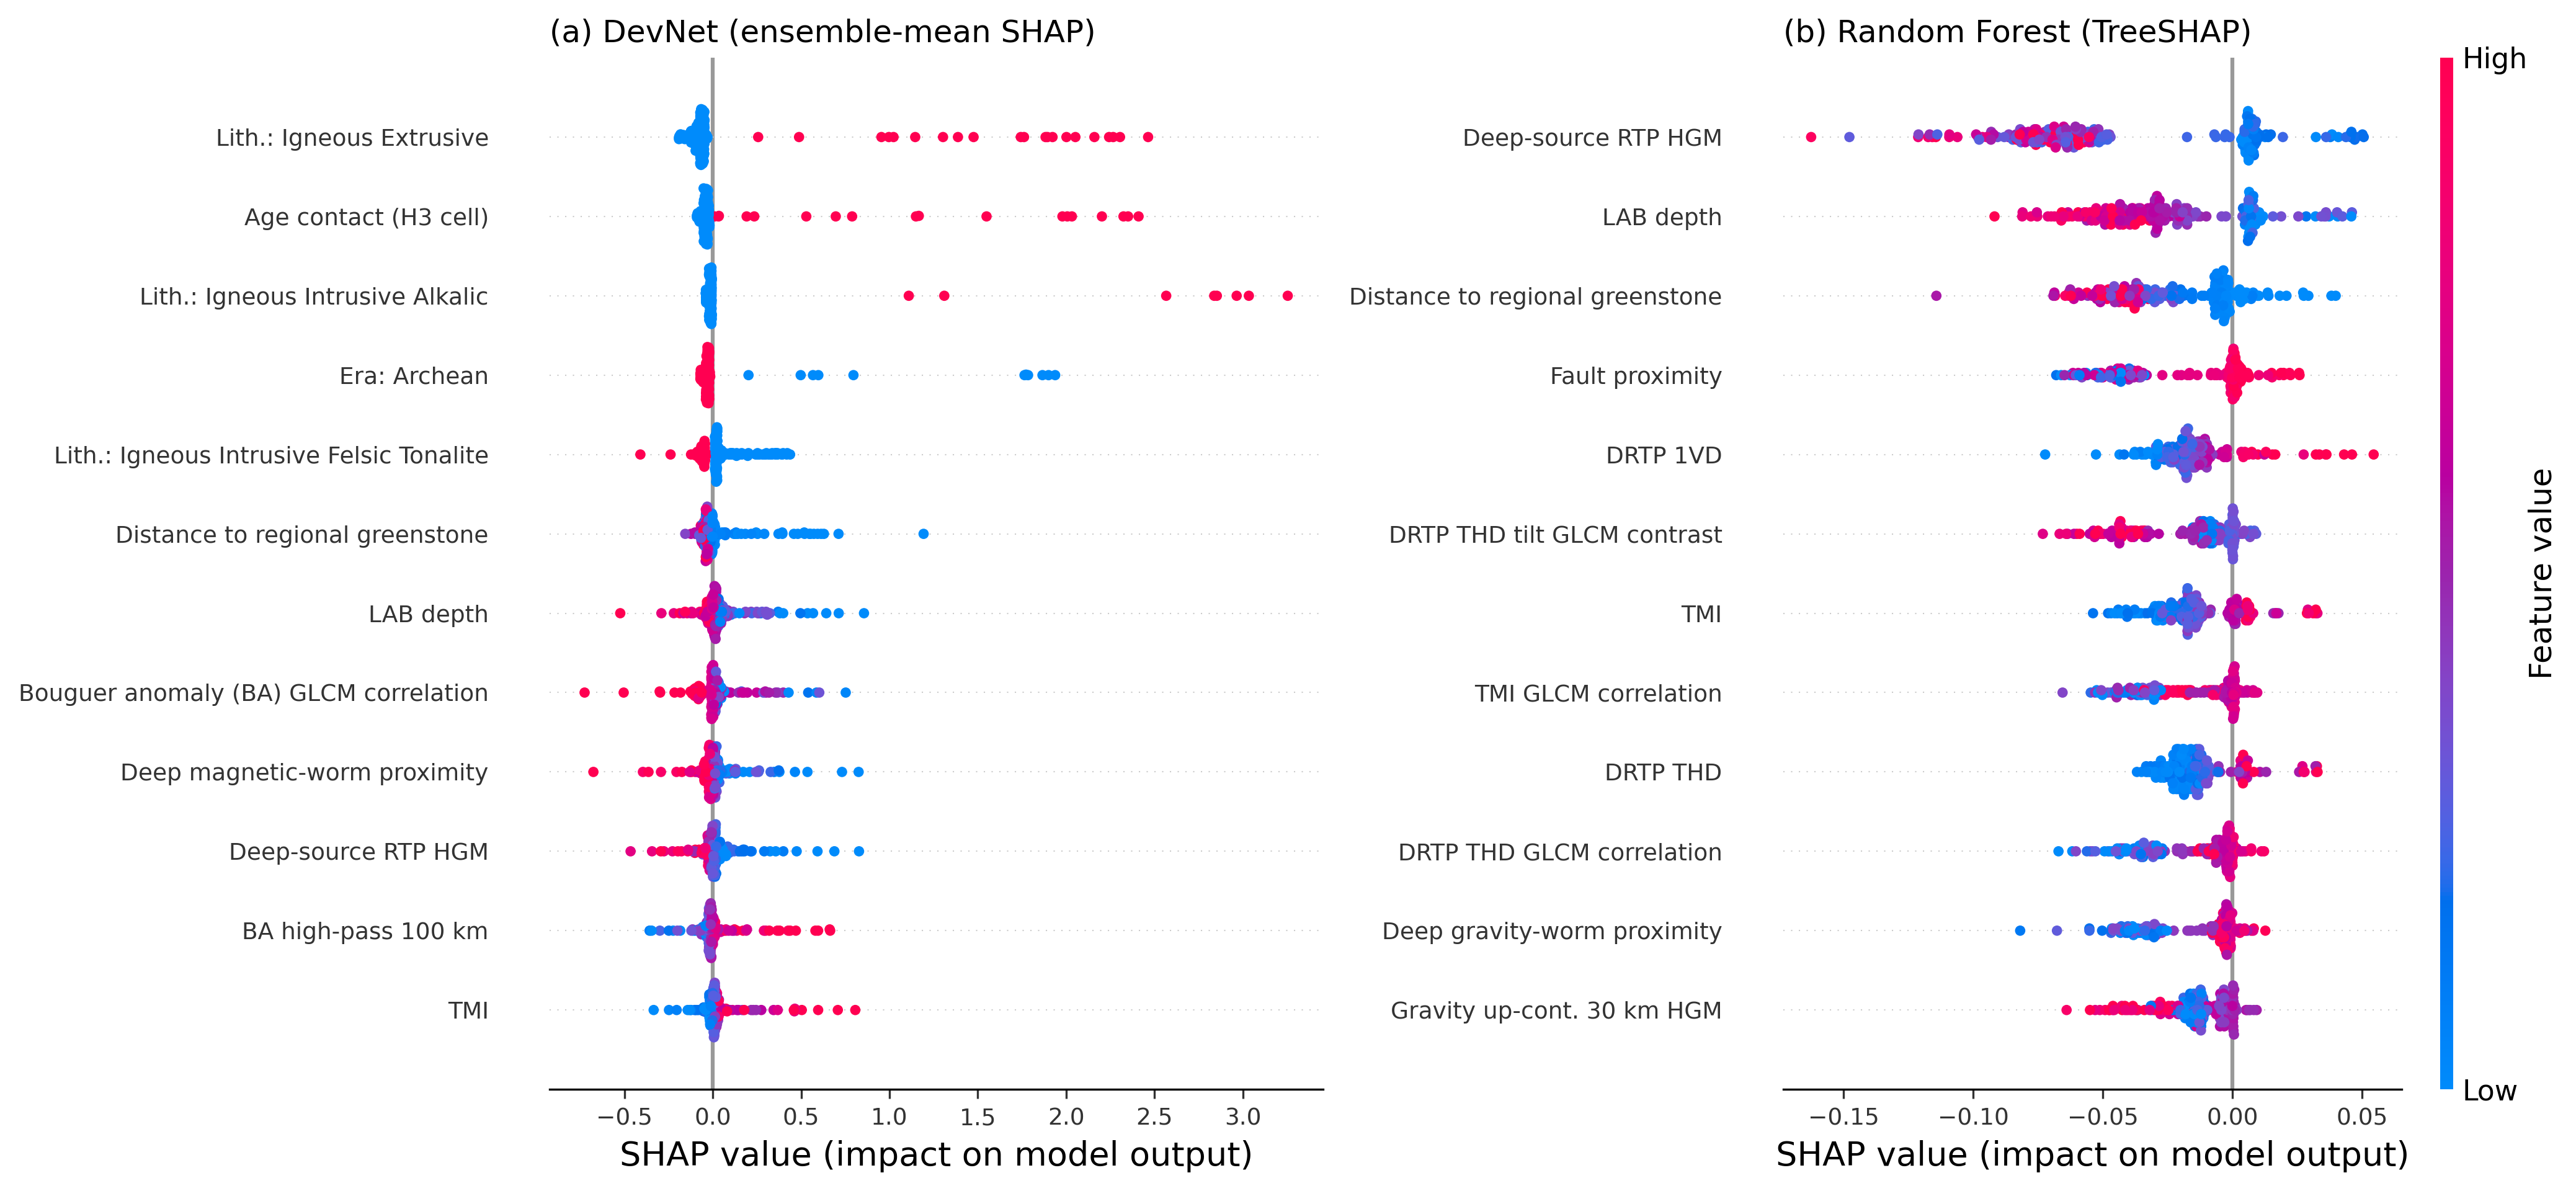
\includegraphics[width=\textwidth]{figures_r7/fig_shap_superior_r2.png}
\caption{苏必利尔省的 SHAP 汇总图：（a）DevNet（在其分位数变换后的输入上计算 DeepSHAP，取五个集成成员的平均）和（b）RF（TreeSHAP）。每个点代表一个被解释样本；颜色表示特征值。SHAP 值的大小在模型之间不可比（无界异常得分与概率）。}\label{fig:shap}
\end{figure}

\begin{table}[t]
\caption{苏必利尔省：两模型共同最重要的十个特征（平均 $|$SHAP$|$，按模型归一化）。排名为在 57 个特征中的名次；方向 $\uparrow$/$\downarrow$：较高值（或存在）提高/降低得分，并给出特征值与 SHAP 值之间的 Spearman $\rho$。}\label{tab:shap}
\scriptsize
\setlength{\tabcolsep}{2.5pt}
\begin{tabular*}{\textwidth}{@{\extracolsep\fill}lcccc}
\toprule
特征 & DevNet 排名 & DevNet 方向 & RF 排名 & RF 方向 \\
\midrule
深源 RTP HGM & 10 & $\downarrow$ (-0.94) & 1 & $\downarrow$ (-0.73) \\
岩性：火成喷出岩 & 1 & $\uparrow$ (+0.53) & 41 & $\uparrow$ (+0.53) \\
LAB 深度 & 7 & $\downarrow$ (-0.93) & 2 & $\downarrow$ (-0.89) \\
到区域绿岩的距离 & 6 & $\downarrow$ (-0.88) & 3 & $\downarrow$ (-0.92) \\
年代接触带（H3 单元） & 2 & $\uparrow$ (+0.50) & 37 & $\uparrow$ (+0.50) \\
岩性：火成侵入碱性岩 & 3 & $\uparrow$ (+0.34) & 22 & $\uparrow$ (+0.34) \\
DRTP 1VD & 13 & $\uparrow$ (+0.95) & 5 & $\uparrow$ (+0.90) \\
TMI & 12 & $\uparrow$ (+0.93) & 7 & $\uparrow$ (+0.91) \\
地质时代：太古宙 & 4 & $\downarrow$ (-0.39) & 24 & $\downarrow$ (-0.39) \\
断层邻近度 & 18 & $\uparrow$ (+0.88) & 4 & $\uparrow$ (+0.87) \\
\botrule
\end{tabular*}
\end{table}

\subsubsection{远景图与外部验证}\label{sec:res-maps}

最终 DevNet 与 RF 远景图（图~\ref{fig:maps}）都将其最高等级集中在苏必利尔省南部、东阿比蒂比矿点群周围以及阿比蒂比和瓦瓦（Wawa）亚省一带，但二者对全省的排序仅中等程度相似（网格上的 Spearman 相关系数为 0.33）。RF 对 80\% 的网格赋予恰好为零的概率，因此其等级取自其余节点。XGBoost 和 bagging-PU（图~\ref{fig:maps-others}）同样把最高等级集中在苏必利尔省南部的东阿比蒂比矿点群周围（与 DevNet 在网格上的 Spearman 相关系数分别为 0.35 和 0.37），而基准测试中最弱的模型 nnPU 则把其前 1\% 的大部分置于该省西北缘和东缘、远离矿点的地方（0.16）。在卡普斯卡辛地区（图~\ref{fig:ksz}），DevNet 将其前 1\% 主要置于 KSZ 以东的阿比蒂比亚省；沿 KSZ 本身，前 5\% 和 10\% 等级在其西侧形成不连续的北北东向斑块。该图幅内最大的前 1\% 斑块位于蒂明斯（Timmins）以北，处于西阿比蒂比亚省 Kidd Creek 铜锌银块状硫化物矿床 \citep{Hannington1999} 周围的绿岩中；该处没有已记录的稀土矿点，这一斑块与 DevNet 所偏好的绿岩环境一致（第~\ref{sec:disc-geology}~节）。Clay-Howells 是位于 KSZ 上、未参与训练的 Fe--REE--Nb 资源，距最近的训练矿点 79~km；在该省 8,000 个随机背景点中，最终模型将其分别置于第 96.6（DevNet）、第 99.8（RF）、第 99.7（XGBoost）、第 94.4（bagging-PU）和第 71.3（nnPU）百分位。

\begin{figure}[t]
\centering
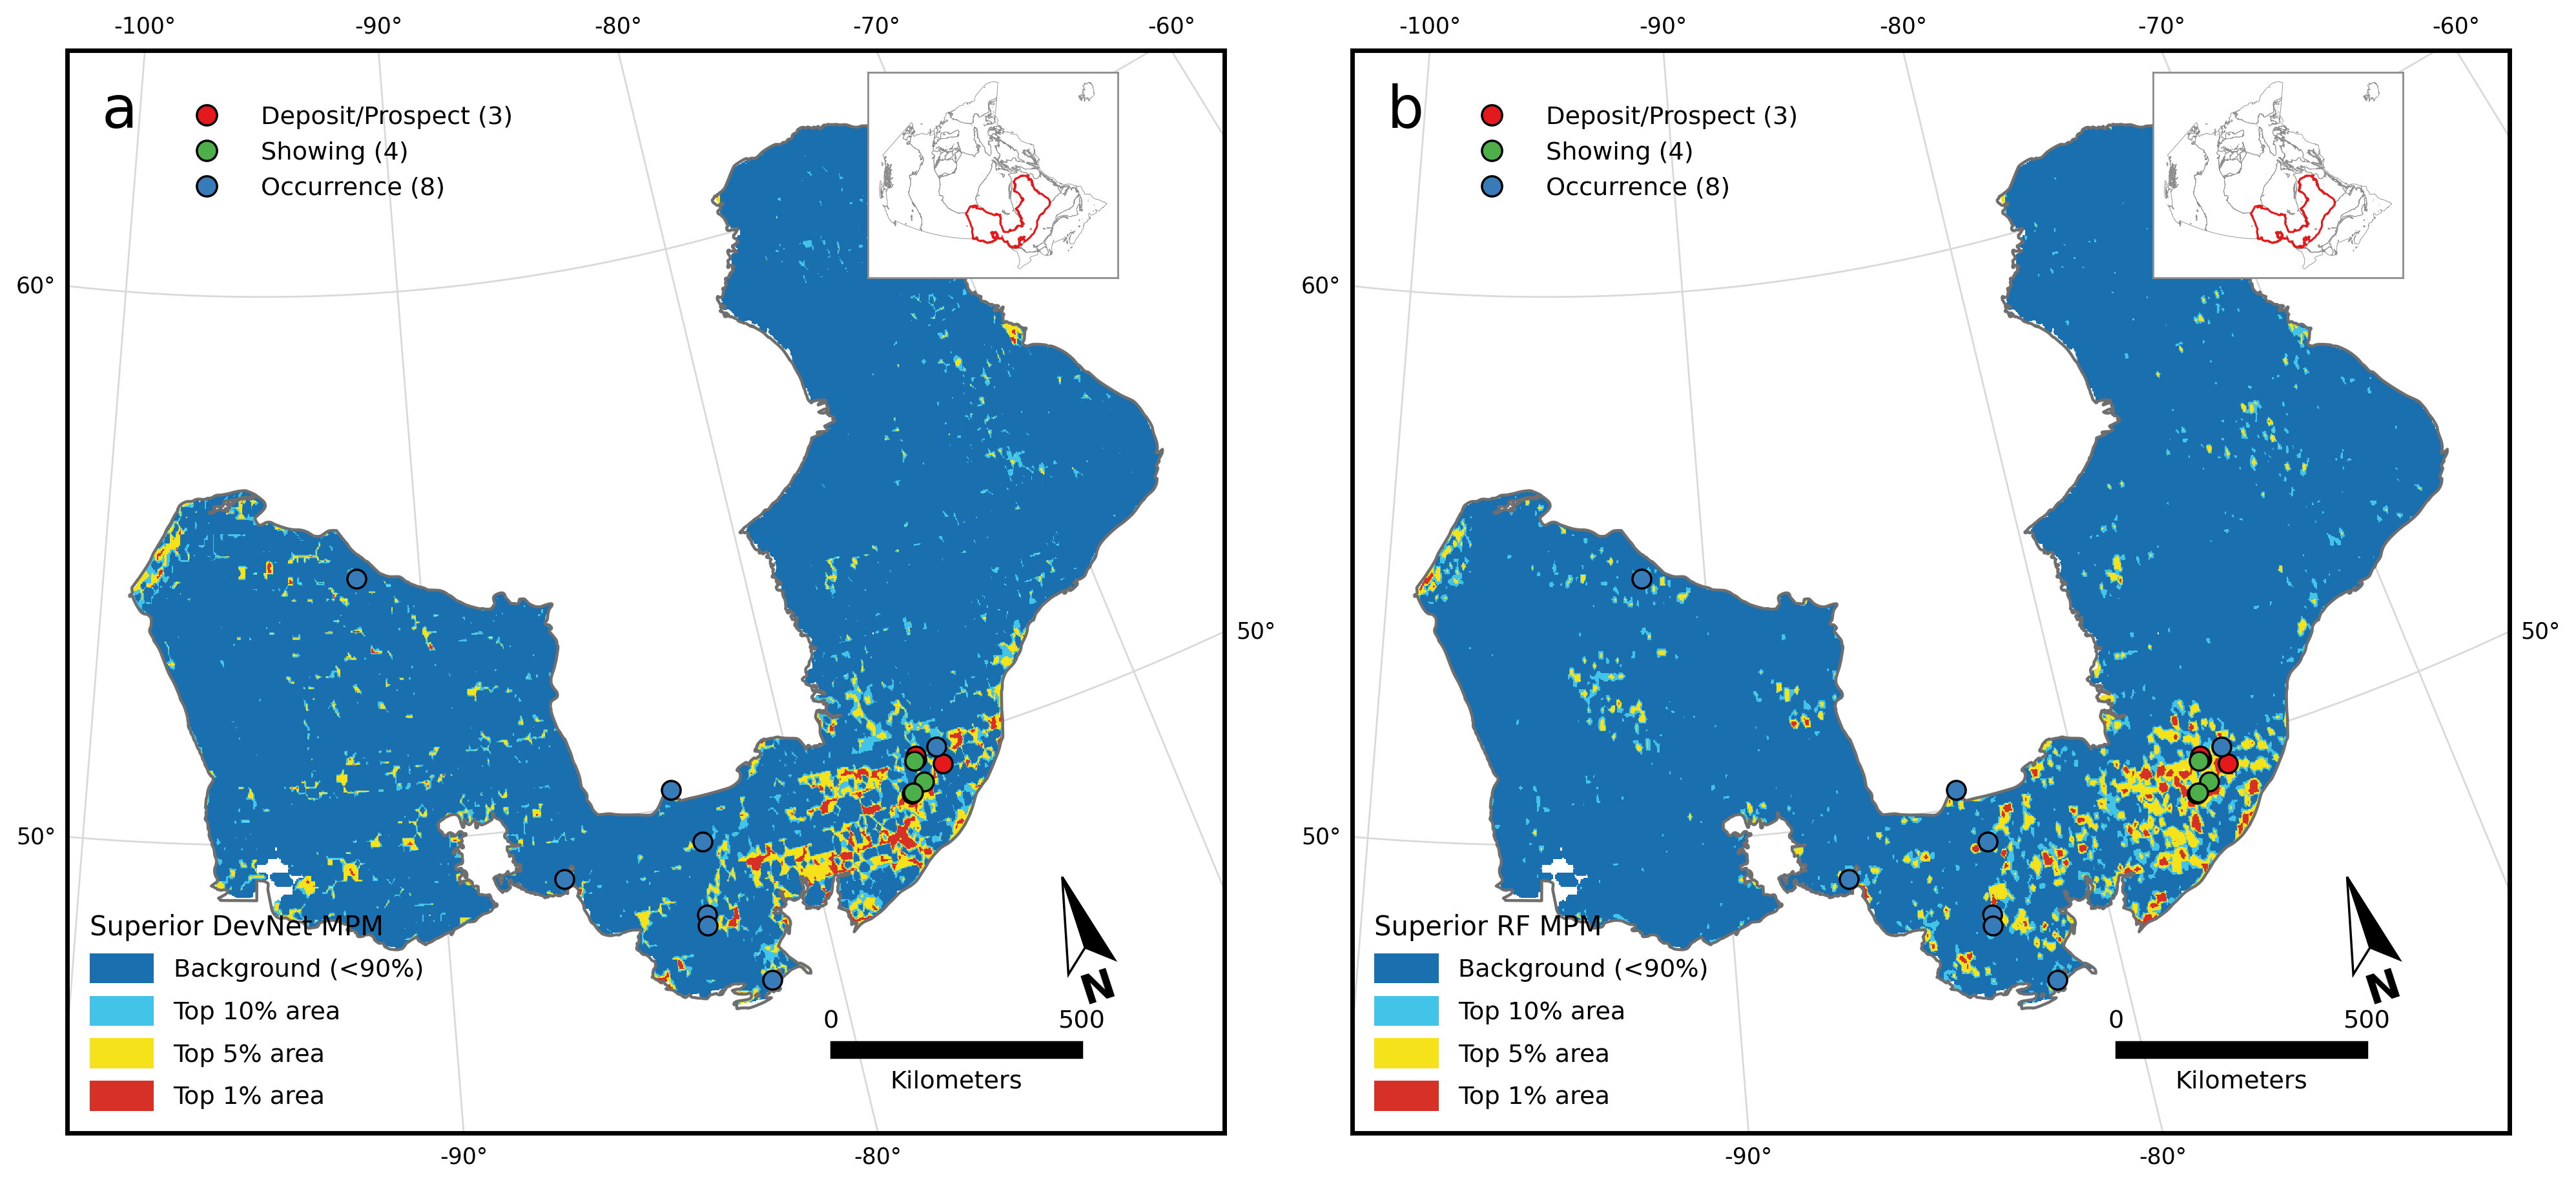
\includegraphics[width=\textwidth]{figures_r7/fig_map_superior_r2.png}
\caption{由最终（a）DevNet 和（b）RF 模型生成的苏必利尔省远景图，按制图区域内的得分百分位分级（前 1\%、5\% 和 10\%），并按开发阶段类别显示已知矿点（Canada Atlas Lambert 投影）。0.1$^\circ$ 预测网格上的得分被插值为 2~km 栅格。}\label{fig:maps}
\end{figure}

\begin{figure}[t]
\centering
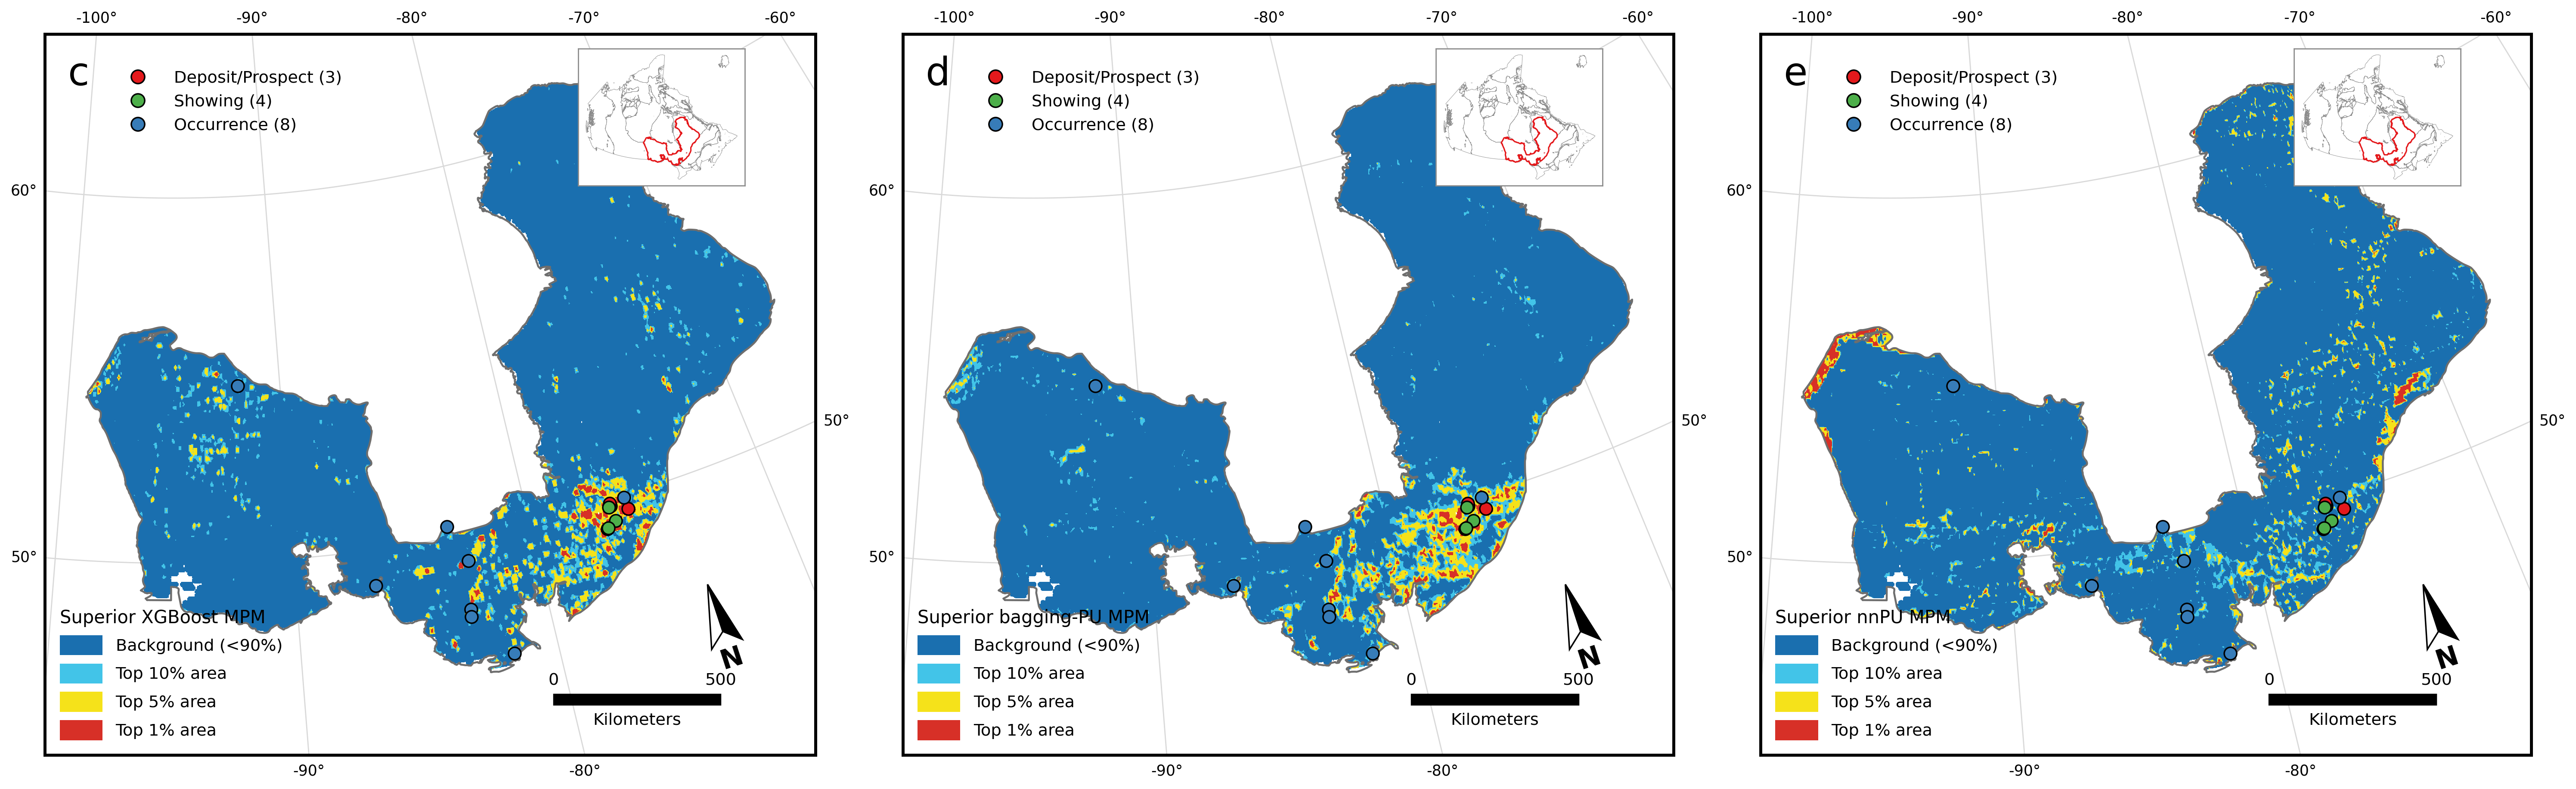
\includegraphics[width=\textwidth]{figures_r7/fig_map_superior_others_r7.png}
\caption{同图~\ref{fig:maps}，为（a）XGBoost、（b）bagging-PU 和（c）nnPU 最终模型的远景图。}\label{fig:maps-others}
\end{figure}

\begin{figure}[t]
\centering
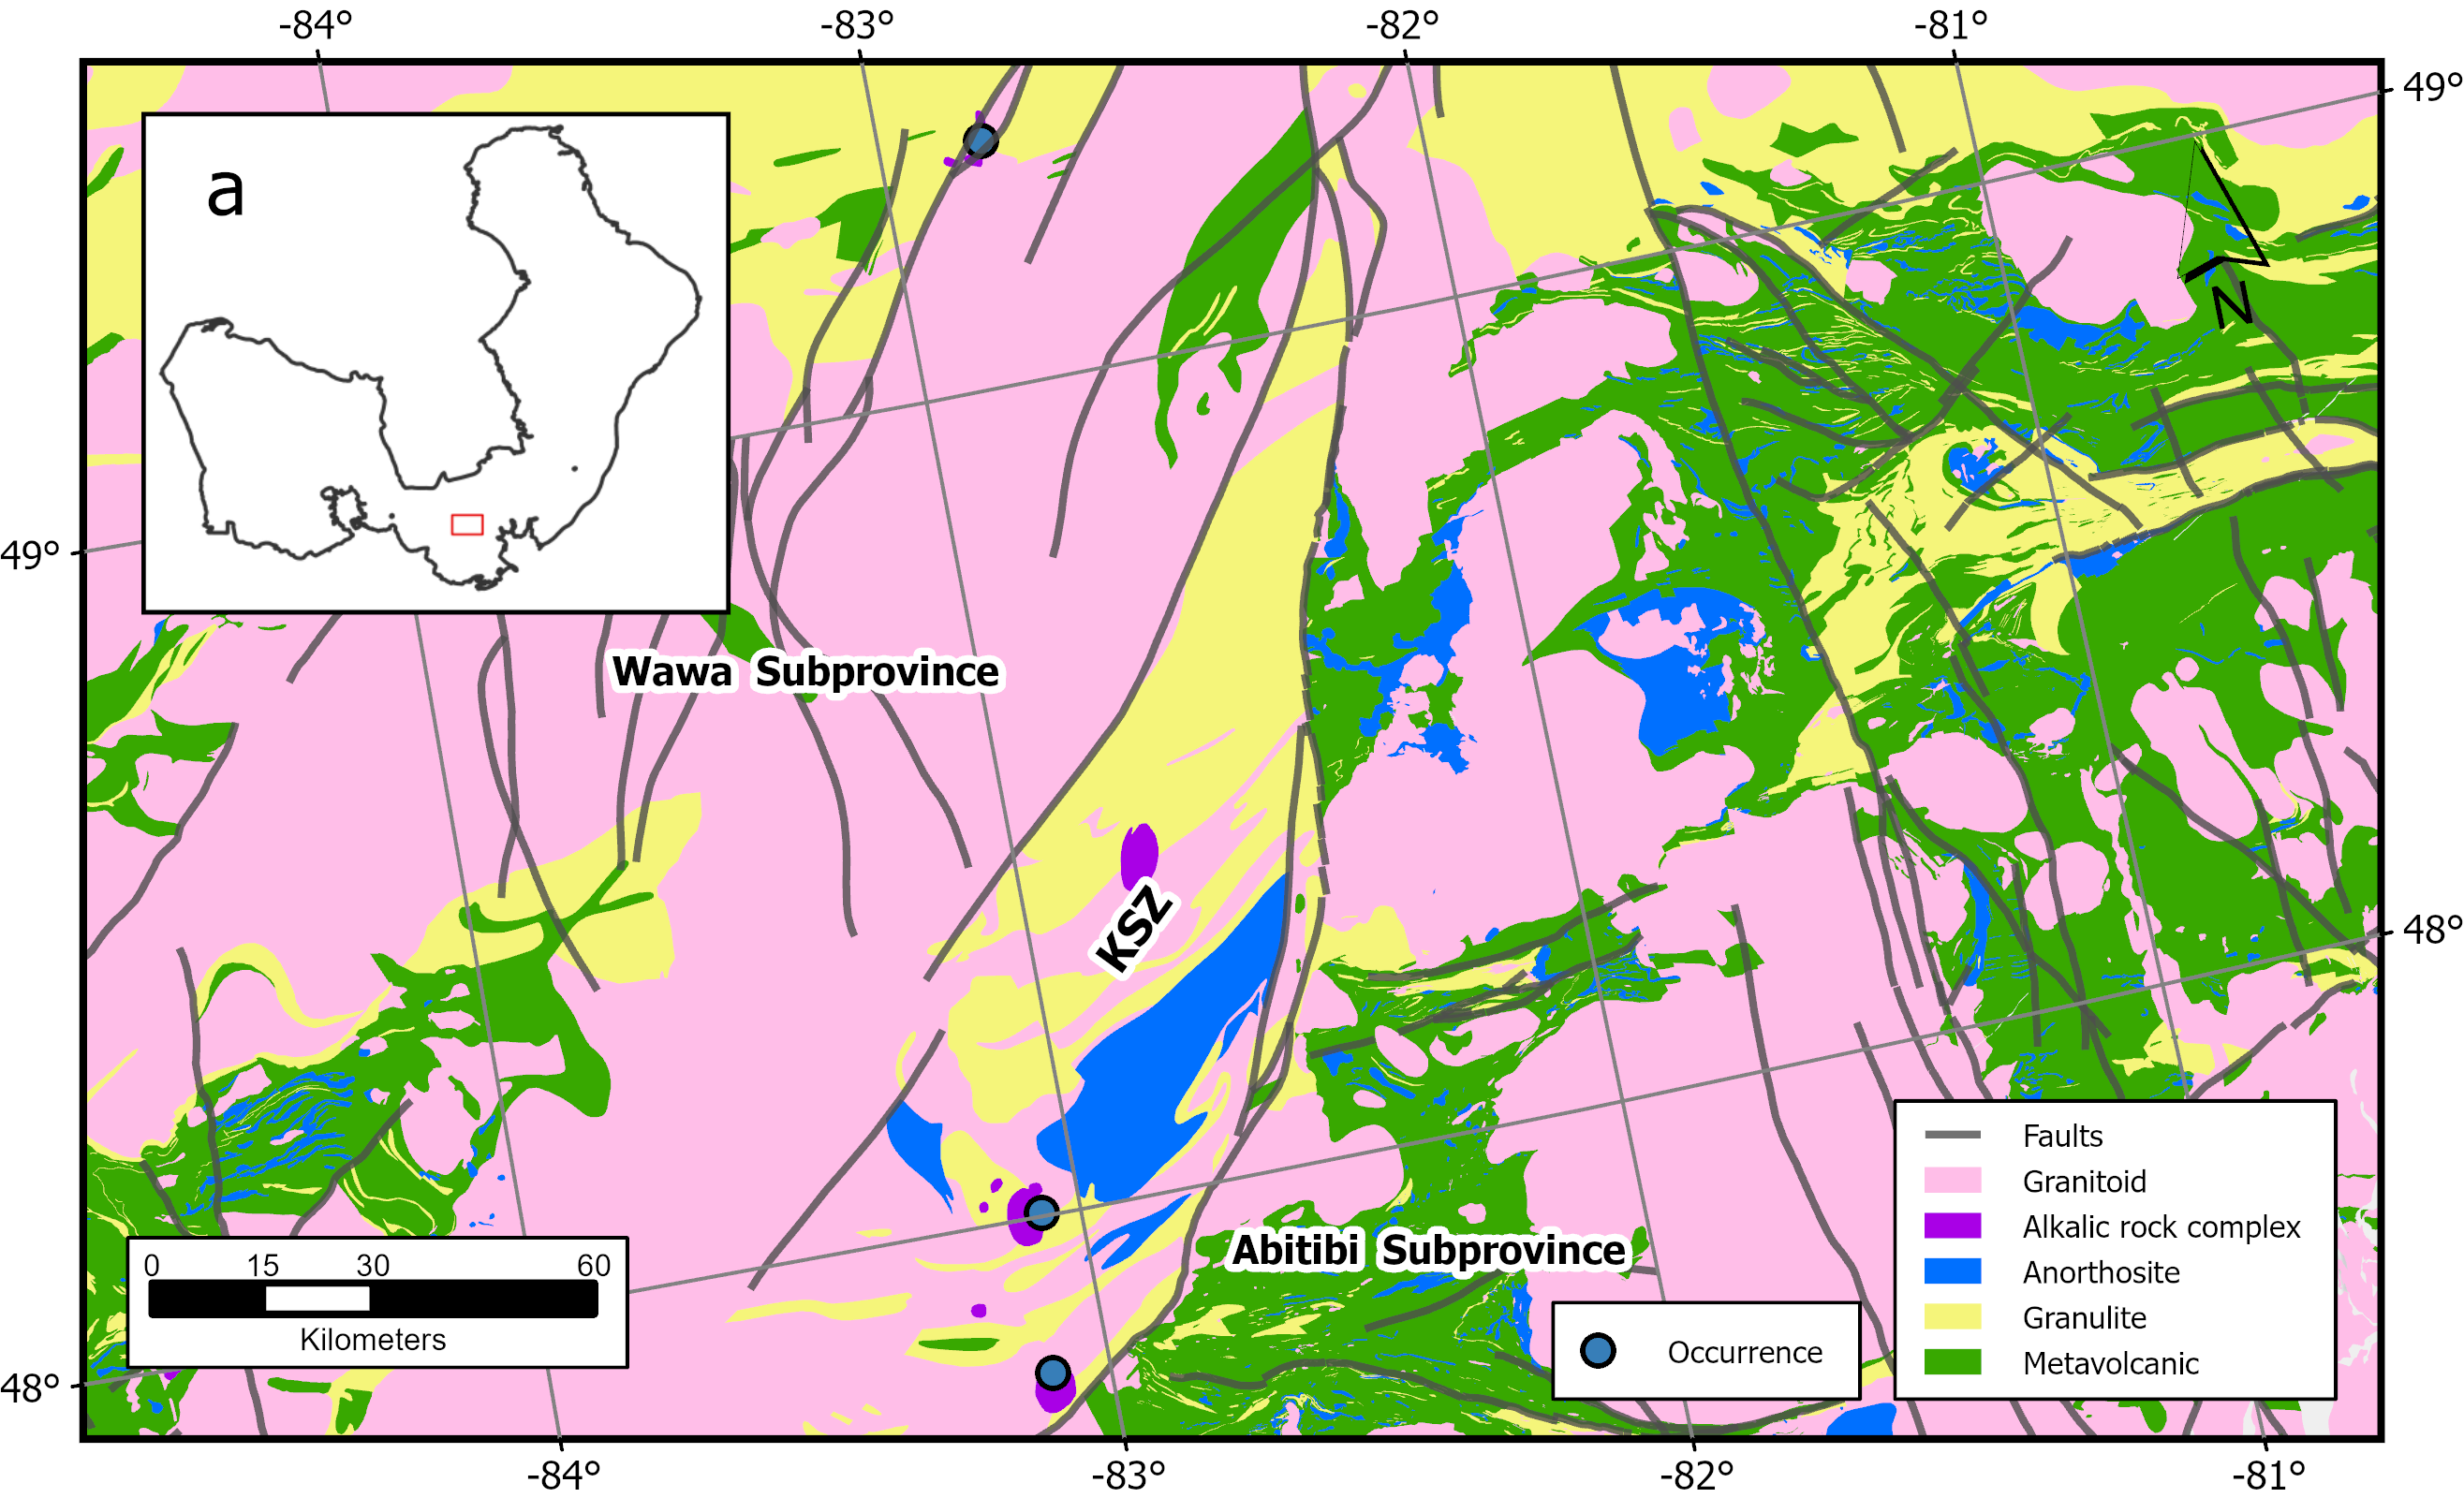
\includegraphics[width=0.49\textwidth]{figures/fig_ksz_geology.png}\hfill
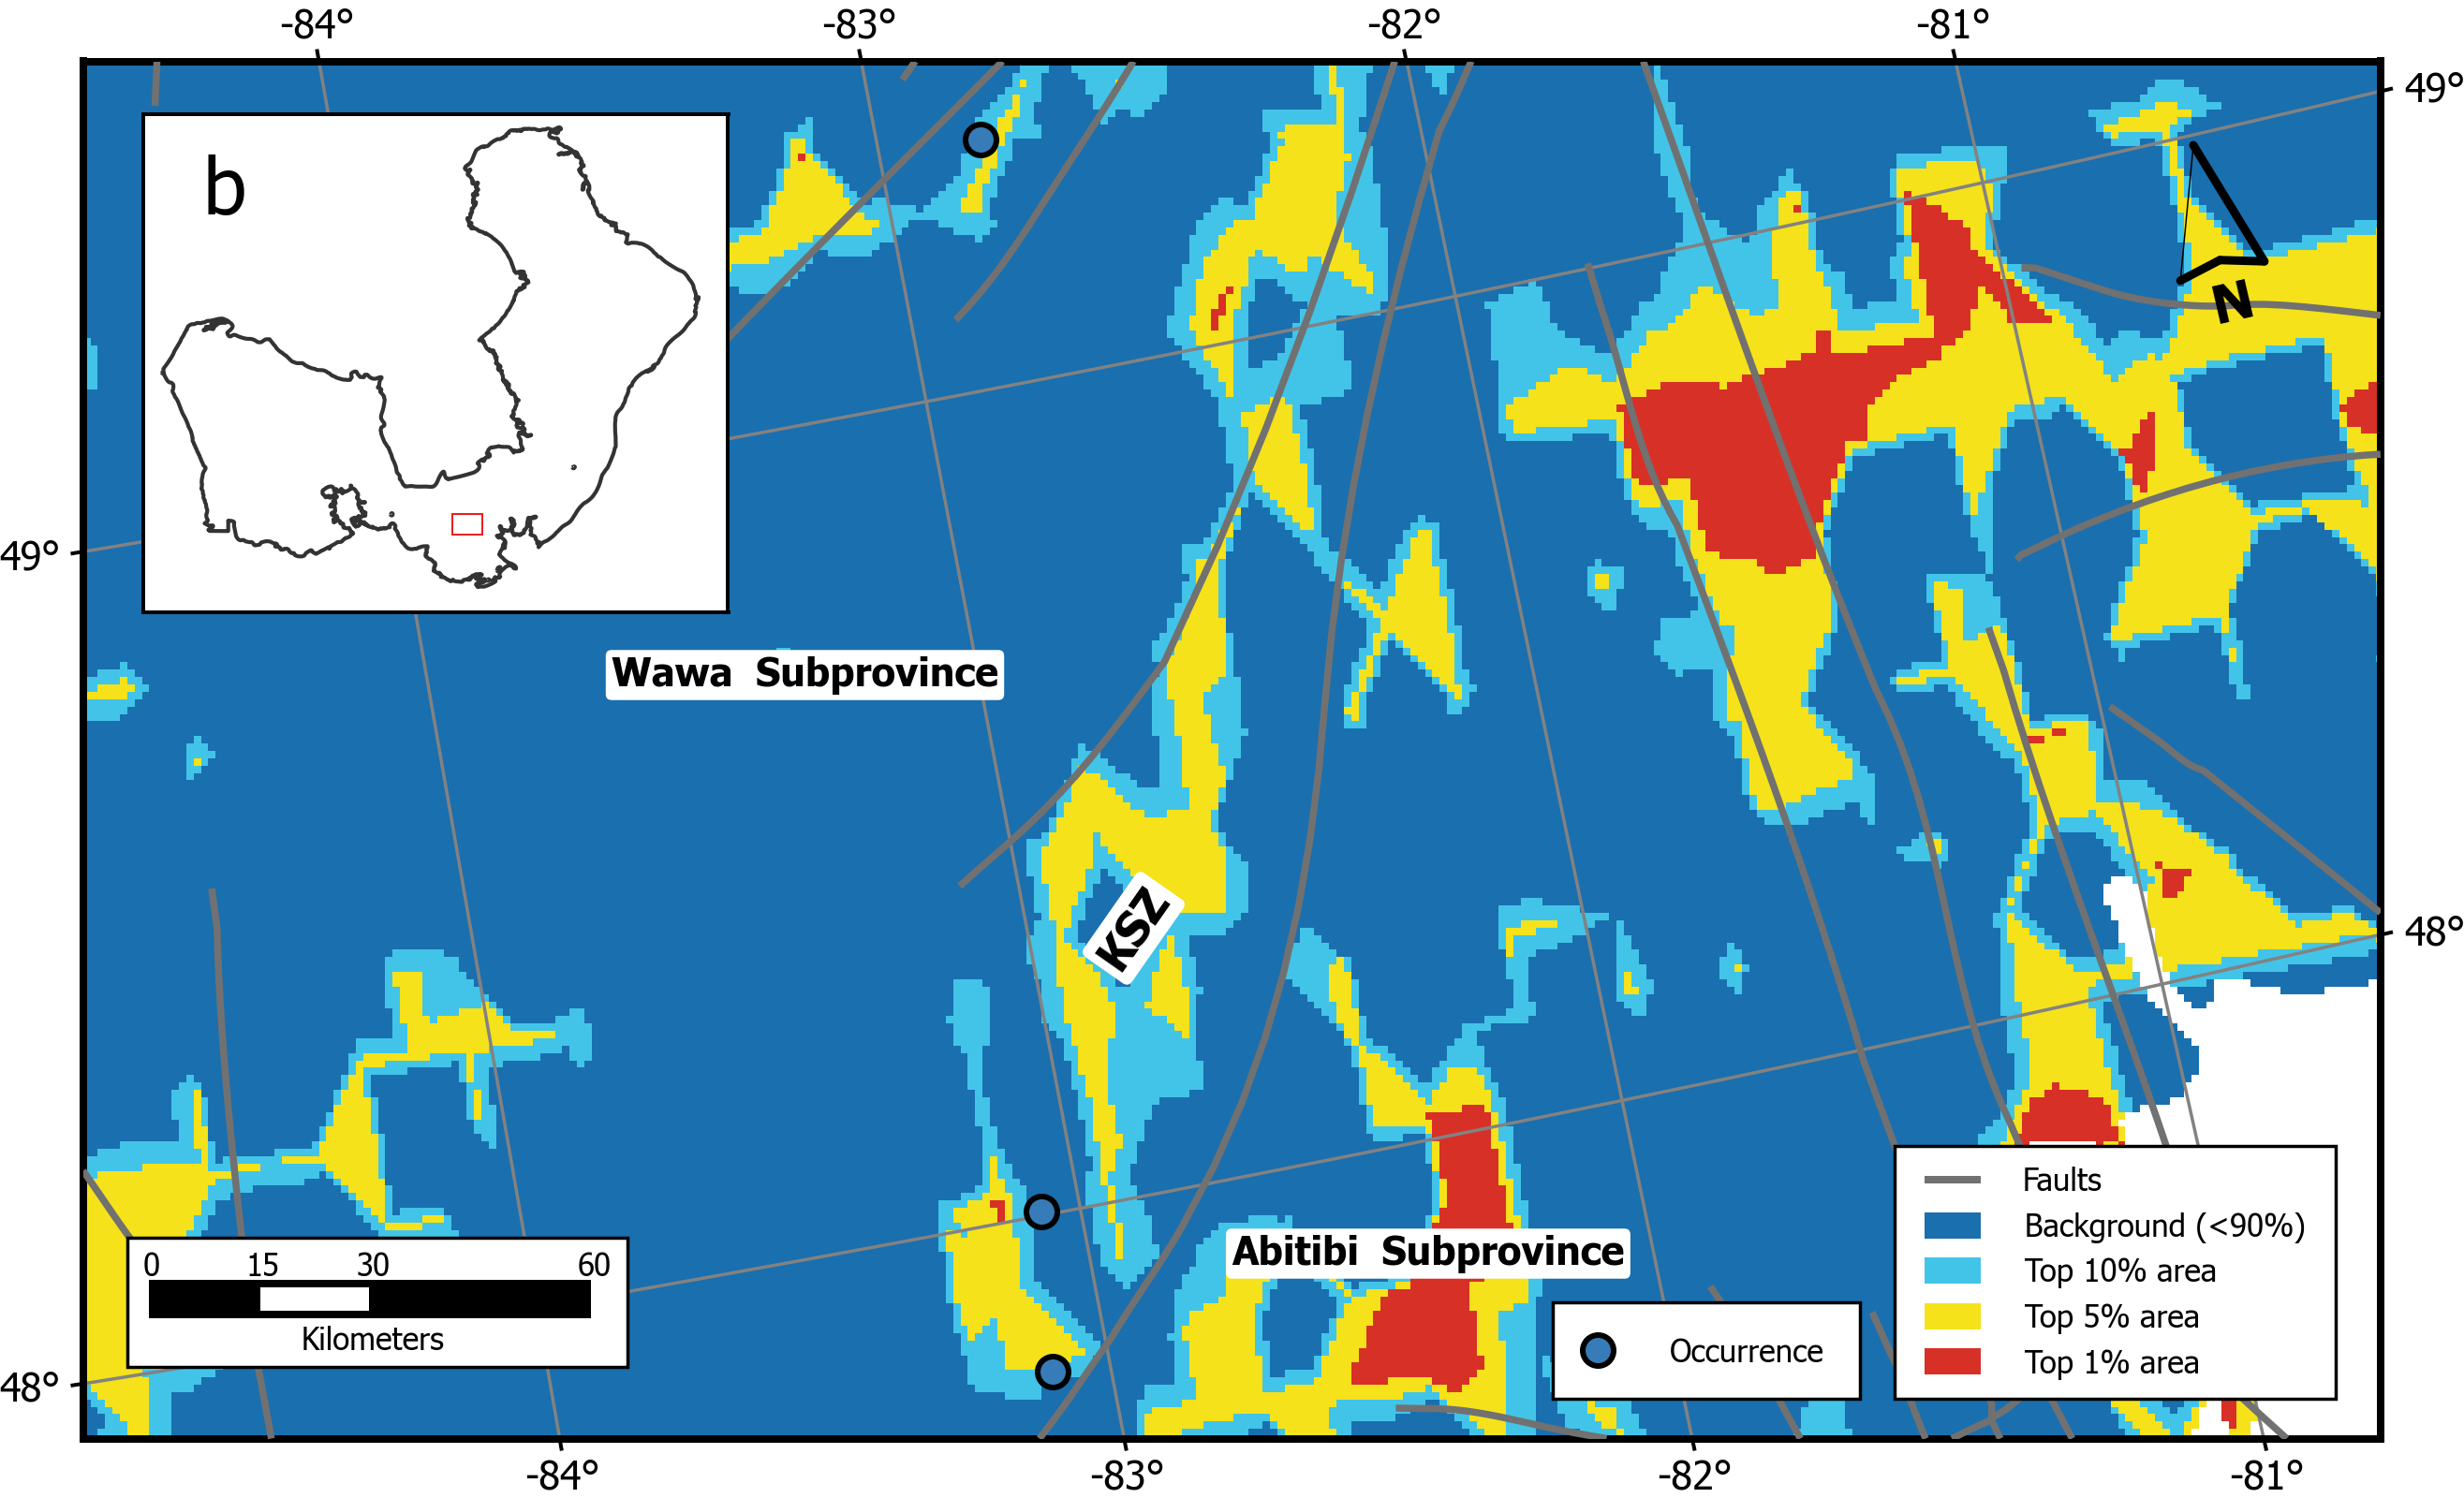
\includegraphics[width=0.49\textwidth]{figures_r7/fig_ksz_r2.png}
\caption{卡普斯卡辛地区。（a）区域地质，示卡普斯卡辛构造带（KSZ）和碱性岩杂岩体 \citep{Gittins1967,Percival1994}，据 \citet{Heather1995} 和 \citet{Montsion2018} 编制。（b）DevNet 前 1\%、5\% 和 10\% 等级（全省范围百分位），叠加用作证据图层的汇编断层，图幅范围与（a）相同。}\label{fig:ksz}
\end{figure}

%% ===================================================================
\section{讨论}\label{sec:discussion}

\subsection{全国尺度模型与迁移能力}\label{sec:disc-scale}

全国尺度的实验和省际迁移检验说明了我们为何对各省分别建模。首先，S2 网格设计的高测试分数并不能衡量在未勘探区域上的预测能力。对增强子单元进行随机划分，会使测试正样本的近似副本留在训练集中；而从相似度最低的区域抽取负样本，恰恰把成矿远景模型最难判断正确的那部分区域排除在评估之外。两者中任一因素单独存在都会使 AUC 接近完美；若每个矿点只取一个标签，并按真实正样本比例随机抽取背景，同一随机森林的 AP 则为 0.29。其次，更大的合并标签集并不能换来迁移能力。各省是可分离的域，若干图层对矿点的指示方向彼此相反（LAB 深度与莫霍面深度、到绿岩的距离），且在一个省训练的模型对另一个省矿点的排序接近甚至低于随机水平。用 \citet{Meyer2021} 的术语来说，一个省位于在另一省训练的模型的适用域（area of applicability）之外；合并数据扩大了训练域，却没有使模型适用于其中的每个部分。全国模型必须从 66 个矿点中同时学习成矿系统的多种表现形式，而省级模型只需学习一种。

\subsection{偏差网络的性能}\label{sec:disc-devnet}

在苏必利尔省，DevNet 在每种验证方案的每次重复中对留出矿点的排序均优于 RF、XGBoost 和 bagging-PU，除两次分块重复外也均优于 nnPU；而且当测试需要外推时，其领先优势最大：RF、XGBoost 和 bagging-PU 在训练正样本周围学习陡峭的决策边界，一旦最近的训练矿点距离达到 50--200~km，它们的 AP 便损失 33--68\%，而 DevNet 直到 100~km 仍保持其大部分 AP。由于只有 15 个正样本，DevNet 相对 RF 的领先幅度并不确定（其 95\% 区间下限低至 0.03），且 DevNet 的设计是在考虑这些省份的情况下选定的；但这一领先在全部 18 个重复-分块组合中都是一致的。

DevNet 的优势并不取决于其两项设计选择（附录~\ref{app:sensitivity}，表~\ref{tab:ablation}）。采用 z-score 标准化的输入、标签平衡的批次或十倍的训练步数时，它在每种验证方案下对留出的苏必利尔省矿点的排序仍远优于 RF（随机划分下 AP 为 0.369--0.417，100~km 分块下为 0.290--0.342，而 RF 分别为 0.268 和 0.129）；最终配置仅在 100 和 200~km 分块下是最佳变体（0.345 和 0.221）。这些变体的共同之处在于偏差损失，以及一个由输入空间中少数几个 ReLU 脊之和构成的得分。当留出矿点远离训练矿点时，这种平滑得分会占优势，而树集成模型的阈值则会切割出每个训练正样本的邻域。

在将背景视为无标签数据的学习器中，真正有效的是偏差损失。nnPU 与 DevNet 使用相同的网络和输入，仅风险函数不同，但在分块验证下其 AP 落后 DevNet 0.13--0.30，在科迪勒拉和格伦维尔省以及去除地质图类别时失效，并且依赖于实际中未知的类别先验（$\pi$ 取 0.005 至 0.05 时 AP 为 0.145--0.275）；bagging-PU 在每种验证方案下都落后于 DevNet。

科迪勒拉和格伦维尔省的结果限定了这一结论的适用范围。在正样本相对较多且呈聚集分布的地区（科迪勒拉），或地球物理信号较弱的地区（格伦维尔省），基于树的学习器在随机划分下表现相当或更好，且没有任何模型能够在分块之间迁移。因此，DevNet 并非判别式基线模型的通用替代品；其优势特定于以下条件的组合：正样本极少、地质背景相同，以及需要在该背景内进行外推。

\subsection{地质图类别：证据与查表}\label{sec:disc-mapclasses}

地质图类别对每个模型的影响都大于模型选择本身的影响。去除这些类别会使 DevNet 和 RF 损失约一半或更多的 AP，而单一类别——碱性侵入岩——贡献了 DevNet 分块 AP 的 30--49\%。苏必利尔省的 15 个矿点中有六个位于被填图为碱性侵入岩的单元上，而该类别覆盖 0.5\% 的背景；对这些矿点而言，地质图本身已经标出了目标。所在单元的年龄接触标志在一定程度上起着同样的作用，因为在太古宙地壳中填图出的元古宙杂岩体会形成年龄接触，而 DevNet 将该特征排在第二位。

这种查表是否可以接受取决于用途。若要在已填图的杂岩体内圈定靶区，或按地球物理背景对已知杂岩体进行排序，已填图的碱性侵入体是合理且有力的证据，使用全部输入是恰当的。若要寻找 1:5,000,000 地质图上未显示的杂岩体，则并非如此，此时相关的预测能力是不含地质图类别时的能力：空间分块下 AP 为 0.075--0.123，是随机排序值的 15--25 倍，但远低于全部输入所显示的水平。研究之间的比较，以及关于模型“发现”矿点能力的论断，都应说明衡量的是两者中的哪一种。在两种情形下，DevNet 在分块验证下都处于或接近最优；然而，其绝对预测能力在很大程度上取决于地质图类别。

\subsection{各省之间的差异}\label{sec:disc-provinces}

对所有模型而言，格伦维尔省都是三个省中表现最弱的，苏必利尔省则最强。各地的证据图层都是相同的全国汇编数据，且几乎完整（各省缺失值均少于 0.01\%），因此这种差异并不反映数据覆盖情况。它反而源于标签集以及这些标签所采样的地质条件。

第一，矿点之间的独立性低于其数量所暗示的程度，在科迪勒拉和格伦维尔省尤为如此：在这两个省，超过一半的矿点距另一矿点不足 10~km（到最近其他矿点距离的中位数为 7~km，而苏必利尔省为 31~km）。在随机划分下，这些相邻矿点会分别落入训练集和测试集，这就是为什么这两个省的随机划分预测能力很高，而在分块下却急剧下降（第~\ref{sec:res-spatial}~节）。

第二，格伦维尔省的标签集混合了不同年龄和构造背景的碳酸岩。Crevier 是约 957~Ma 的晚格伦维尔期碱性岩-碳酸岩侵入体 \citep{Groulier2020}。St-Honoré（同一杂岩体上还有 Terres Rompues）约于 580~Ma 侵位于圣劳伦斯（St.~Lawrence）裂谷系的萨格奈（Saguenay）地堑中 \citep{Neron2018}。Lavergne--Springer 矿点位于渥太华-邦尼谢尔（Ottawa--Bonnech\`ere）地堑西端的尼皮辛湖（Lake Nipissing）附近，而加蒂诺（Gatineau）附近的 Cantley、Quinnville 和 Templeton 矿化点属于格伦维尔大理岩带中的富方解石脉和岩墙，其岩浆成因长期存在争议 \citep{Moecher1997}。仅年龄的多样性并不是问题所在，因为苏必利尔省的矿点也跨越了多个岩浆期次 \citep{Rukhlov2010}。然而，它们全部侵位于同一个稳定的克拉通岩石圈中，而现今的 LAB、莫霍面和位场图层仍记录着该岩石圈的边缘和地壳尺度构造。格伦维尔省的地壳经历了格伦维尔造山作用和后期裂谷作用的改造，因此对于形成于不同背景的矿点，其现今的地球物理特征未必记录了一个共同的背景。填图地质还引入了其自身的噪声：十二个格伦维尔省矿点落在太古宙、元古宙和古生代地质图单元上，因为基岩地质图记录的是改造后的原岩以及覆盖在 St-Honoré 之上的古生代盖层，而非碳酸岩本身；并且其中没有一个位于被填图为碱性侵入岩的单元上，而格伦维尔省约 5\% 的背景位于这类单元上。在更大尺度上，同样是缺乏共同背景，导致模型无法在省际迁移（第~\ref{sec:res-transfer}~节）。

因此，地球物理数据的缺失或粗糙对这种差异的解释力很小；差异的大部分可由标签的数量、独立性和地质一致性来解释。格伦维尔省的模型要么需要更多同一类型碳酸岩的矿点，要么需要针对裂谷相关型和造山型分别建模，而现有标签集无法支持这两种做法。

\subsection{正样本增强与标签稀缺}\label{sec:disc-gan}

正样本增强是应对标签稀缺的一种颇具吸引力的方法，且已有研究恰好针对这一矿种推荐使用 GAN 生成的标签 \citep{Parsa2025}。我们的结果提示应持谨慎态度。用十余个训练正样本拟合的生成器有两种选择。它可以紧贴这些正样本，此时它添加的是不携带任何新信息的近似重复样本（抖动和 SMOTE，最近邻距离比为 0.1--0.2）；它也可以向外扩散，此时它必须猜测未见矿点所在的位置，而由于没有这方面的任何信息，它会将一部分概率质量置于类似背景的特征空间中（WGAN-GP，37\% 的样本的最近邻为背景点）。两种选择都无法提供真正缺失的信息，即未发现的矿点是什么样子。RF 的增益更适合解释为平滑效应：训练正样本周围及其之间的增强点使更多的树对其附近的留出点投正类票，这使 RF 由恰为零的概率构成的退化曲面得到缓解，而不是教会它新的地质知识。扩散最远的 WGAN-GP 样本对 RF 帮助最大，在 200~km 分块下同样如此，但即使是最佳的增强 RF 也仍远低于未经增强的 DevNet（100~km 分块下为 0.191 对 0.345）；而 DevNet 的损失函数本身就能产生平滑得分，它从同样的增强点中获益甚微且不稳定。在使用正样本增强时，增强正样本必须在每个训练折内仅由该折的正样本生成，且性能必须在真实的留出矿点上衡量；否则，测试集中某个训练矿点的增强副本会以另一种形式重现第~\ref{sec:res-ladder}~节中的兄弟单元问题。

\subsection{验证设计与所报告的性能}\label{sec:disc-protocol}

我们的发现中有四项涉及的是评估而非模型本身。第一，当正样本只有数十个时，单次交叉验证划分给出的估计噪声很大：对同一套苏必利尔省（Superior Province）数据重新划分，会使每个模型的 AP 在 0.06--0.11 的范围内变动（表~\ref{tab:benchmark}），与模型之间的许多差异同样大。第二，只要矿点呈聚集分布，随机划分就会高估模型能力，而且高估的程度因模型而异，因此随机划分还可能颠倒模型的排序（第~\ref{sec:res-spatial}~节）。第三，在全国尺度上重建后，S2 网格设计的两个分类器均给出 1.000 的测试 AUC，而该设计中有两个要素抬高了这一数值：一是从最不相似的区域抽取负样本，仅此一项即已足够（不做增强时分别为 0.998 和 0.996）；二是对增强子单元进行随机划分，因为几乎每个测试正样本在训练一侧都有一个兄弟单元，二者的粗分辨率深部结构变量值和地质图类别完全相同，细尺度变量值也几乎相同（使用随机负样本时，随机森林为 0.997，CNN 为 0.937；而将兄弟单元保持在同一侧时分别为 0.923 和 0.880）。在这种设计下，留出测试实际上是要求模型识别一个它已经见过的位置；\citet{Parsa2024} 曾用训练 AUC 与测试 AUC 的比较来论证其模型没有过拟合，但由于测试集并不独立于训练集，这种比较也就失去了信息量。\citet{Parsa2024} 所报告的增强带来的提升，有一部分正是这种泄漏所致：在我们的数据上，随机划分时增强使 CNN 的类别平衡测试 AUC 从 0.824 升至 0.937，而将兄弟单元保持在一起时仅升至 0.880（随机森林：0.882、0.997 和 0.923）。从最不相似的 5\% 区域中选取负样本，又引入了第二个相互独立的乐观偏差来源：它恰恰把远景模型最难判断正确的那部分区域排除在评估之外。第四，地质图类别可以通过标出已知杂岩体而贡献所报告能力中的很大一部分（第~\ref{sec:disc-mapclasses}~节），而这一点是任何划分设计都无法消除的。

我们要强调全国实验能说明什么、不能说明什么。该实验使用的是我们的输入和标签，配以 \citet{Parsa2024} 的两个分类器，其中该研究未报告的设置由我们补全，且未采用其针对随机森林的网格搜索；因此，它并不能确定在分组划分下他们的结果会是多少。但它确实表明：在加拿大全国碳酸岩数据上，已发表的设计无论使用哪个分类器都会得到 1.000 的测试 AUC，而在每个矿点一个标签、随机背景和真实正样本比例的条件下，随机森林的 AUC 为 0.903、AP 为 0.292，CNN 的 AUC 为 0.852、AP 为 0.059；它还表明，在一个省训练的模型无法推广到另一个省。无论是高 AUC 还是其在不同划分之间的小幅波动，都不能作为模型可推广至未勘探区域的证据。\citet{Parsa2025} 在一个加入 GAN 生成标签的工作流程中描述了同样的 70/30 分层随机划分；其描述并未说明由某一原始标签派生出的增强标签是否与该标签被划分在同一侧。若并非如此，上述警示就更为适用。因此，对于标签极度稀缺条件下的成矿远景研究，我们建议：（i）在任何划分之前，将每个增强标签或近似重复标签与其来源矿点归为同一组；（ii）从研究区域中随机抽取评估负样本，而不是从与正样本最不相似的区域中抽取；（iii）报告多次重复划分下的 AP 及其区间，而非单一的 AUC；（iv）增加一种空间分块验证，并从留出分块中剔除训练背景；（v）同时报告包含与不包含点位地质图类别的结果，使读者能够看出得分中有多少来自地图查表；（vi）对于跨地质省汇总训练的模型，检验其向留出省份的迁移能力，并在固定的地质单元内计算依赖于范围的输入。

\subsection{地质解释}\label{sec:disc-geology}

RF 与 DevNet 在苏必利尔省一致认定的控制因素描绘了一个自洽的地质背景。较浅的 LAB，加之深源磁梯度的重要性排名靠前，指向厚的苏必利尔岩石圈根边缘处较薄的岩石圈；在那里，交代地幔的低程度熔融以及沿岩石圈尺度构造的上升通道最有可能出现 \citep{Griffin2013,Groves2021,Hoggard2020}；阿比蒂比南部之下的一个地幔导电体与这种交代作用相吻合 \citep{Snyder2021}。断层邻近度和高磁场强度捕捉到了汇聚岩浆上升的构造以及含磁铁矿侵入体本身 \citep{Thomas2016}。靠近深部磁力蠕虫的负效应则不那么直观；它可能反映了深部磁性接触带集中分布于那些本身并非碳酸岩赋存部位的地体边界，不应对其过度解读。

绿岩岩性以及靠近区域绿岩单元所表现出的强正效应需要更谨慎地看待。15 个矿点中有八个属于位于以绿岩为主的亚省内的阿比蒂比东部矿点群，因此这种关联可能部分记录的是最大矿点群的所在位置，而非分散矿点所共有的控制因素；在分块条件下被 DevNet 排序最低的分散矿点——Kapuskasing 和 Nemegosenda Lake——位于 KSZ 的高级变质地体和碱性地体中，而不是位于绿岩带中。与此一致，DevNet 的远景图仅以不连续的斑块形式沿 KSZ 分布，而位于 KSZ 上、未参与训练的 Clay-Howells 资源仍排在其第 97 百分位。一个最高远景等级与某一个绿岩赋存矿点群紧密关联的模型，适用于对该类型区域进行排序，但不应期望它能同样好地识别其他地质背景中的碱性杂岩体。

\subsection{局限性}\label{sec:limitations}

十五个正样本只能支撑较弱的统计结论：我们的可靠结果是那些在各次重复、各种分块尺寸、各项比较和各个省份之间均保持一致的结果。DevNet 的输入表示和批次构成是借助在这三个省上的诊断性实验选定的，尽管在当前输入下，每种变体对苏必利尔省矿点的排序均优于 RF（附录~\ref{app:sensitivity}）；仍需在一个独立的省份上加以验证，而最明显的候选——丘吉尔省——在去重后所含的碳酸岩型矿点过少，无法进行有意义的检验。本文所用的地质编码是在对一种较粗的岩性分组进行评估之后才取代该分组的；这一更改在随机划分和 50--100~km 分块下提高了除 nnPU 以外所有模型的 AP，但在 200~km 分块下则没有。评估背景中可能包含尚未发现的矿点，因此所有指标均为下限。放射性测量数据因覆盖不完整而无法使用，全岩地球化学数据又过于稀疏，无法作为输入。化极假设磁化为感应磁化；具有剩余磁化的地质体无法被正确化极。断层汇编数据的来源应在发表前对照原始数据发布进行确认。矿点类别信息（矿床/远景区 Deposit/Prospect、矿化显示 Showing、矿点 Occurrence）未用于加权；由于每类仅有 3--8 个矿点，无法可靠地评估基于置信度加权的训练。最后，远景图给出的是各区域内的百分位，而非经过校准的概率。在全国尺度上，66 个矿点中有 12 个位于三个研究省之外，其中四个构成一个矿点群（Ashram），因此“加拿大其余地区”这一组样本量小且存在空间依赖性；全国标签来自两份汇编：一项并行的全国研究所使用的第三份汇编 \citep{Huston2024} 会额外增加一个矿床（Hoidas Lake），而 \citet{Orris2018} 中碳酸岩亲缘性被标为不确定、已被我们排除的五条记录会再增加五个（其中之一是作为我们外部检验的 Clay-Howells）；此外，0.1$^\circ$ 格网在高纬度地区单位面积上的采样更密。

%% ===================================================================
\section{结论}\label{sec:conclusions}

针对加拿大碳酸岩型稀土的成矿远景预测，在全国共有 66 个矿点、各省 12--27 个矿点的条件下：
\begin{enumerate}
\item 在这些数据上重建后，\citet{Parsa2024} 的全国 S2 网格设计在其随机森林和 CNN 上均给出 1.000 的测试 AUC；仅从最不相似的区域抽取负样本即足以达到这一结果（不做增强时分别为 0.998 和 0.996），而仅对增强子单元进行随机划分就能将随机森林提升至 0.997。在每个矿点一个标签、随机背景和真实正样本比例的条件下，随机森林的 AUC 为 0.903、AP 为 0.292，CNN 的 AUC 为 0.852、AP 为 0.059。
\item 在苏必利尔省（Superior Province），无论在随机交叉验证还是 50--200~km 空间分块交叉验证下，半监督偏差网络（DevNet）对留出矿点的排序均优于随机森林（RF）、XGBoost、bagging-PU 和 nnPU（AP 分别为 0.38 和 0.37--0.22，而 RF 和 XGBoost 为 0.27 和 0.18--0.09），且相对于 RF、XGBoost 和 bagging-PU 在每一次重复中均如此；在仅有 15 个矿点的情况下，其相对于 RF 的领先是一致的，但领先幅度尚不确定。这一优势不依赖于 DevNet 的输入缩放方式或批次构成。
\item 地质图类别对每个模型的影响都大于模型选择本身。单一一个已填图的碱性侵入体类别覆盖了苏必利尔省 15 个矿点中的 6 个和 0.5\% 的背景，却承载了 DevNet 分块 AP 的 30--49\%；若去掉点位地质图类别，DevNet 和 RF 会损失约一半甚至更多的预测能力。成矿远景研究应同时报告包含和不包含此类类别的结果。
\item 在科迪勒拉造山带和格伦维尔省（Grenville Province），基于树的学习器在随机划分下领先，而且没有任何模型能在分块之间迁移；造成这一反差的是标签的数量、独立性和地质一致性，而非数据覆盖程度。
\item 采用抖动、SMOTE 或表格型 WGAN-GP 进行的正样本增强（严格在训练折内生成）没有给 DevNet 带来一致的提升；它提高了 RF 的 AP（以 WGAN-GP 的提升最大），但并未使其接近未增强的 DevNet。
\item 模型无法在地质省之间迁移：在大多数情况下，一个省的模型对另一个省矿点的排序处于或低于随机水平；各省在证据图层中是可区分的；而且若干图层在不同省份中对矿点的指示方向相反。因此，针对这些矿点的远景模型应分省构建。
\item RF 与 DevNet 对三个省全部 30 个主要控制因素的作用方向判断一致。DevNet 的苏必利尔省远景图将未参与训练的 Clay-Howells Fe--REE--Nb 资源置于其第 97 百分位，并偏向于类似占主导地位的阿比蒂比矿点群那样的绿岩赋存环境。
\end{enumerate}

\backmatter

\bmhead{致谢}
本工作始于在帝国理工学院（Imperial College London）完成的一项理学硕士（MSc）独立研究项目。我们感谢 Ross Smail、Chetan Nathwani 教授和 Rebecca Bell 教授的指导，并感谢 Junlin Fang 在方法与模型评估方面的讨论。

\section*{声明}

\bmhead{资助} %% TODO(author)
不适用。

\bmhead{利益冲突} %% TODO(author)
作者声明不存在任何利益冲突。

\bmhead{数据可用性}
矿点标签来源于 \citet{Orris2018} 和 \citet{Parsa2024}；去重后的省级和全国矿点表以及研究区边界随代码一同发布。所有证据图层均为公开数据，可从 \citet{McCafferty2023}、\citet{Jobin2017}、\citet{Miles2016}、\citet{BradleyDC2008} 和 \citet{Wheeler1996} 获取；派生的重力和磁力网格可由代码复现。

\bmhead{代码可用性} %% TODO(author): make the repository public or archive it (e.g. Zenodo) before submission
本流程、本文中的每一项分析以及生成文中表格和图件的脚本均可在 \url{https://github.com/miaozhou-312/ree-prospectivity-paper} 获取。

\begin{appendices}

\section{补充结果}\label{app:full}

\begin{table}[!h]
\caption{表~\ref{tab:spatial} 中各组运行的 AUC（六次重复的中位数）。粗体：每行中最高的 AUC。}\label{tab:spatial-auc}
\footnotesize
\setlength{\tabcolsep}{3pt}
\begin{tabular*}{\textwidth}{@{\extracolsep\fill}llccccc}
\toprule
区域 & 划分方式 & DevNet & RF & XGBoost & Bagging-PU & nnPU \\
\midrule
\multirow{4}{*}{苏必利尔省} & 随机 & 0.972 & \textbf{0.985} & 0.976 & 0.976 & 0.842 \\
 & 50 km & 0.969 & \textbf{0.976} & 0.962 & 0.964 & 0.862 \\
 & 100 km & \textbf{0.928} & 0.922 & 0.904 & 0.921 & 0.846 \\
 & 200 km & \textbf{0.886} & 0.861 & 0.826 & 0.837 & 0.819 \\
\midrule
\multirow{4}{*}{科迪勒拉} & 随机 & 0.925 & 0.936 & 0.926 & \textbf{0.937} & 0.575 \\
 & 50 km & 0.866 & 0.856 & 0.840 & \textbf{0.879} & 0.581 \\
 & 100 km & 0.747 & 0.841 & 0.782 & \textbf{0.856} & 0.565 \\
 & 200 km & 0.744 & 0.720 & 0.712 & \textbf{0.825} & 0.584 \\
\midrule
\multirow{4}{*}{格伦维尔省} & 随机 & 0.826 & 0.836 & 0.870 & \textbf{0.909} & 0.609 \\
 & 50 km & 0.755 & 0.717 & 0.777 & \textbf{0.825} & 0.620 \\
 & 100 km & 0.699 & 0.687 & 0.722 & \textbf{0.780} & 0.598 \\
 & 200 km & 0.681 & 0.582 & 0.665 & \textbf{0.691} & 0.609 \\
\botrule
\end{tabular*}
\end{table}

\begin{table}[!h]
\caption{nnPU 对假定类别先验 $\pi$ 的敏感性，苏必利尔省（随机交叉验证；六次重复的中位数及 95\% 区间）。}\label{tab:prior}
\footnotesize
\begin{tabular*}{0.6\textwidth}{@{\extracolsep\fill}lcc}
\toprule
$\pi$ & AUC & AP \\
\midrule
0.005 & 0.823 [0.761, 0.860] & 0.145 [0.079, 0.177] \\
0.01 & 0.842 [0.772, 0.873] & 0.159 [0.096, 0.210] \\
0.02 & 0.864 [0.827, 0.897] & 0.195 [0.115, 0.251] \\
0.05 & 0.885 [0.878, 0.919] & 0.275 [0.186, 0.395] \\
\botrule
\end{tabular*}
\end{table}

\clearpage
\section{正样本增强：生成器与空间分块}\label{app:aug-spatial}

\begin{figure}[!h]
\centering
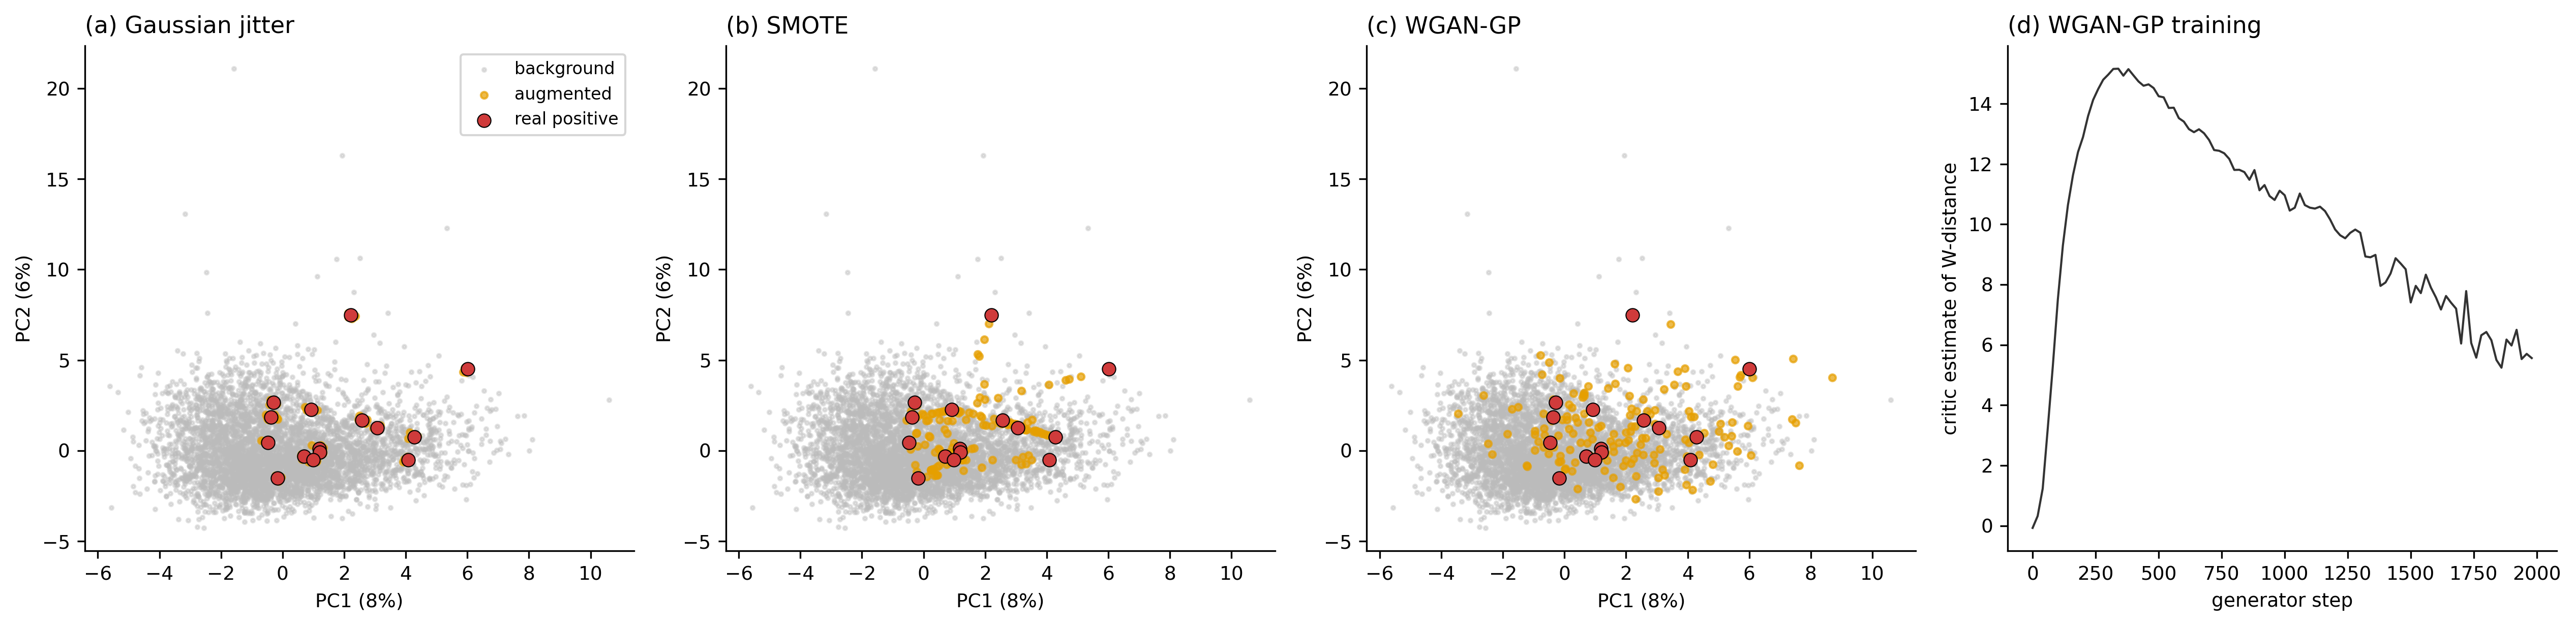
\includegraphics[width=\textwidth]{figures_r7/fig_augmentation_superior_r4.png}
\caption{（a--c）各生成器（基于苏必利尔省全部 15 个正样本拟合）生成的增强正样本在背景样本与真实正样本前两个主成分空间中的分布。（d）训练过程中 WGAN-GP 判别器（critic）对 Wasserstein 距离的估计。}\label{fig:aug-pca}
\end{figure}

\begin{table}[!h]
\caption{空间分块交叉验证下采用折内安全（fold-safe）正样本增强时苏必利尔省的平均精度（六次重复的中位数及 95\% 区间）。DevNet 的运行在另一台机器上完成；其训练在不同机器之间并非逐位一致，因此其未增强结果与表~\ref{tab:spatial} 在小数点后第三位上存在差异。}\label{tab:aug-spatial}
\footnotesize
\begin{tabular*}{0.7\textwidth}{@{\extracolsep\fill}lllc}
\toprule
分块 & 模型 & 增强方式 & AP \\
\midrule
100 km & DevNet & 无 & 0.343 [0.163, 0.414] \\
 &  & 高斯抖动 10$\times$ & 0.341 [0.156, 0.420] \\
 &  & SMOTE 3$\times$ & 0.324 [0.146, 0.418] \\
 &  & WGAN-GP 3$\times$ & 0.326 [0.228, 0.398] \\
 &  & WGAN-GP 10$\times$ & 0.308 [0.172, 0.350] \\
\addlinespace
100 km & RF & 无 & 0.129 [0.067, 0.161] \\
 &  & 高斯抖动 10$\times$ & 0.139 [0.074, 0.187] \\
 &  & SMOTE 3$\times$ & 0.110 [0.053, 0.168] \\
 &  & WGAN-GP 3$\times$ & 0.135 [0.074, 0.202] \\
 &  & WGAN-GP 10$\times$ & 0.191 [0.083, 0.294] \\
\addlinespace
200 km & DevNet & 无 & 0.216 [0.154, 0.310] \\
 &  & 高斯抖动 10$\times$ & 0.238 [0.157, 0.314] \\
 &  & SMOTE 3$\times$ & 0.200 [0.155, 0.251] \\
 &  & WGAN-GP 3$\times$ & 0.246 [0.165, 0.314] \\
 &  & WGAN-GP 10$\times$ & 0.258 [0.171, 0.305] \\
\addlinespace
200 km & RF & 无 & 0.087 [0.053, 0.149] \\
 &  & 高斯抖动 10$\times$ & 0.096 [0.062, 0.137] \\
 &  & SMOTE 3$\times$ & 0.077 [0.047, 0.118] \\
 &  & WGAN-GP 3$\times$ & 0.132 [0.080, 0.199] \\
 &  & WGAN-GP 10$\times$ & 0.122 [0.074, 0.256] \\
\botrule
\end{tabular*}
\end{table}

\clearpage
\section{对比省份中的模型解释}\label{app:shap}

\begin{table}[!h]
\caption{同表~\ref{tab:shap}，科迪勒拉（61 个特征）。}\label{tab:shap-cord}
\footnotesize
\begin{tabular*}{\textwidth}{@{\extracolsep\fill}lcccc}
\toprule
特征 & DevNet 排名 & DevNet 方向 & RF 排名 & RF 方向 \\
\midrule
到区域高级变质岩的距离 & 5 & $\downarrow$ (-0.96) & 1 & $\downarrow$ (-0.86) \\
地质时代：元古宙 & 2 & $\uparrow$ (+0.59) & 19 & $\uparrow$ (+0.70) \\
地质时代：中生代 & 4 & $\downarrow$ (-0.82) & 11 & $\downarrow$ (-0.82) \\
布格重力异常（BA） & 9 & $\downarrow$ (-0.96) & 3 & $\downarrow$ (-0.87) \\
年代接触带（H3 单元） & 1 & $\uparrow$ (+0.84) & 44 & $\uparrow$ (+0.84) \\
DRTP THD GLCM 相关性 & 3 & $\downarrow$ (-0.82) & 27 & $\downarrow$ (-0.42) \\
莫霍面深度 & 8 & $\uparrow$ (+0.96) & 6 & $\uparrow$ (+0.91) \\
到区域绿岩的距离 & 17 & $\uparrow$ (+0.93) & 4 & $\uparrow$ (+0.34) \\
被动陆缘邻近度 & 41 & $\uparrow$ (+0.28) & 2 & $\uparrow$ (+0.81) \\
到区域年代接触带的距离 & 7 & $\uparrow$ (+0.95) & 14 & $\uparrow$ (+0.92) \\
\botrule
\end{tabular*}
\end{table}

\begin{table}[!h]
\caption{同表~\ref{tab:shap}，格伦维尔省（66 个特征）。}\label{tab:shap-gren}
\footnotesize
\begin{tabular*}{\textwidth}{@{\extracolsep\fill}lcccc}
\toprule
特征 & DevNet 排名 & DevNet 方向 & RF 排名 & RF 方向 \\
\midrule
到区域年代接触带的距离 & 9 & $\downarrow$ (-0.96) & 1 & $\downarrow$ (-0.79) \\
深源 RTP & 5 & $\uparrow$ (+0.93) & 2 & $\uparrow$ (+0.73) \\
DRTP THD 倾斜角 & 10 & $\downarrow$ (-0.95) & 3 & $\downarrow$ (-0.83) \\
DRTP THD 倾斜角 GLCM 对比度 & 1 & $\downarrow$ (-0.94) & 10 & $\downarrow$ (-0.93) \\
BA THD 倾斜角 GLCM 对比度 & 4 & $\uparrow$ (+0.97) & 5 & $\uparrow$ (+0.83) \\
到区域镁铁质-超镁铁质岩的距离 & 24 & $\uparrow$ (+0.92) & 4 & $\uparrow$ (+0.42) \\
到区域沉积岩的距离 & 15 & $\downarrow$ (-0.95) & 6 & $\downarrow$ (-0.90) \\
DRTP 均值（10 km） & 6 & $\uparrow$ (+0.95) & 9 & $\uparrow$ (+0.93) \\
莫霍面深度 & 22 & $\downarrow$ (-0.92) & 7 & $\downarrow$ (-0.69) \\
深部磁力蠕虫邻近度 & 3 & $\uparrow$ (+0.97) & 25 & $\uparrow$ (+0.79) \\
\botrule
\end{tabular*}
\end{table}

\clearpage
\section{DevNet 设计选择的消融实验}\label{app:sensitivity}

本附录使用主分析的输入检验 DevNet 的两项设计选择（第~\ref{sec:models}~节）：以采用 z-score 标准化输入和 16 + 16 行标签平衡批次的配置为起点，每次只改变一个要素。所有配置均采用与主要结果相同的折、评估方案和随机种子进行评估（表~\ref{tab:ablation}）。在苏必利尔省，各变体之间差别不大，且没有任何一种在所有评估方案下都是最优的：在随机划分下，z-score 输入配合以背景为主的批次获得最高的 AP（0.417，最终配置为 0.381）；在 50~km 分块下，标签平衡批次最优（0.390 和 0.384，最终配置为 0.371）；在 100 和 200~km 分块下，最终配置最高（0.345 和 0.221）。所有变体均远高于 RF（0.268、0.165、0.129 和 0.087；表~\ref{tab:spatial}）。延长训练会反复使用这十几个正样本，促使网络倾向于记忆其邻域：在 z-score 输入下，将训练步数增加到十倍提高了随机划分下的 AP（0.401 对比 0.369），却降低了 100~km 分块下的 AP（0.290 对比 0.329）。嵌套早停配置在每个外层训练折内部通过 100~km 空间交叉验证（三个内层折、两次内层重启，并从内层验证分块中剔除背景）选择训练步数（100--3,000，在 3,000 步上采用余弦调度），因此测试折从不参与这一选择。表~\ref{tab:margin} 给出了最终配置对偏差间隔（margin）的敏感性：较小的间隔在苏必利尔省和科迪勒拉获得了更高的 AP（苏必利尔省在 $a = 2$ 时为 0.472，在 $a = 5$ 时为 0.381），但在格伦维尔省并非如此；我们沿用 \citet{Pang2019} 的取值，而不在这些折上对其进行调优。

\begin{table}[!h]
\caption{DevNet 设计选择的消融实验：在相同折上，随机交叉验证和空间分块下的 AP（六次重复的中位数）。输入：分位数-正态变换或 z-score 标准化；批次：每步的正样本\,+\,背景行数；步数：梯度步数（嵌套 ES：通过嵌套 100~km 空间交叉验证选择）。粗体：最终配置。--：未运行。}\label{tab:ablation}
\scriptsize
\setlength{\tabcolsep}{2.5pt}
\begin{tabular*}{\textwidth}{@{\extracolsep\fill}llllllll}
\toprule
区域 & 输入 & 批次 & 步数 & 随机 & 50 km & 100 km & 200 km \\
\midrule
\multirow{6}{*}{苏必利尔省} & 分位数 & 16\,+\,240 & 300（最终） & \textbf{0.381} & \textbf{0.371} & \textbf{0.345} & \textbf{0.221} \\
 & z-score & 16\,+\,240 & 300 & 0.417 & 0.378 & 0.342 & 0.212 \\
 & 分位数 & 16\,+\,16 & 300 & 0.397 & 0.384 & 0.329 & 0.220 \\
 & z-score & 16\,+\,16 & 300 & 0.369 & 0.390 & 0.329 & 0.201 \\
 & z-score & 16\,+\,16 & 3,000 & 0.401 & -- & 0.290 & -- \\
 & z-score & 16\,+\,16 & 嵌套 ES & 0.401 & 0.358 & 0.297 & 0.190 \\
\midrule
\multirow{6}{*}{科迪勒拉} & 分位数 & 16\,+\,240 & 300（最终） & \textbf{0.327} & \textbf{0.131} & \textbf{0.048} & \textbf{0.056} \\
 & z-score & 16\,+\,240 & 300 & 0.303 & 0.136 & 0.074 & 0.049 \\
 & 分位数 & 16\,+\,16 & 300 & 0.307 & 0.124 & 0.045 & 0.052 \\
 & z-score & 16\,+\,16 & 300 & 0.273 & 0.135 & 0.077 & 0.045 \\
 & z-score & 16\,+\,16 & 3,000 & 0.255 & -- & 0.060 & -- \\
 & z-score & 16\,+\,16 & 嵌套 ES & 0.284 & 0.140 & 0.069 & 0.047 \\
\midrule
\multirow{6}{*}{格伦维尔省} & 分位数 & 16\,+\,240 & 300（最终） & \textbf{0.127} & \textbf{0.036} & \textbf{0.008} & \textbf{0.007} \\
 & z-score & 16\,+\,240 & 300 & 0.113 & 0.030 & 0.007 & 0.006 \\
 & 分位数 & 16\,+\,16 & 300 & 0.113 & 0.031 & 0.008 & 0.008 \\
 & z-score & 16\,+\,16 & 300 & 0.078 & 0.026 & 0.009 & 0.008 \\
 & z-score & 16\,+\,16 & 3,000 & 0.129 & -- & 0.010 & -- \\
 & z-score & 16\,+\,16 & 嵌套 ES & 0.107 & 0.022 & 0.008 & 0.008 \\
\botrule
\end{tabular*}
\end{table}

\begin{table}[!h]
\caption{DevNet 对偏差间隔 $a$ 的敏感性（AP，六次重复的中位数，随机交叉验证）。主要结果采用 $a = 5$。}\label{tab:margin}
\footnotesize
\begin{tabular*}{0.7\textwidth}{@{\extracolsep\fill}lcccc}
\toprule
区域 & $a = 2$ & $a = 3$ & $a = 5$ & $a = 8$ \\
\midrule
苏必利尔省 & 0.472 & 0.446 & 0.381 & 0.377 \\
科迪勒拉 & 0.367 & 0.379 & 0.327 & 0.313 \\
格伦维尔省 & 0.126 & 0.115 & 0.127 & 0.120 \\
\botrule
\end{tabular*}
\end{table}

\end{appendices}

\clearpage

\bibliography{references}

\end{document}
